% --- PREAMBLE ------------------------------------------------------
\documentclass[12pt, oneside]{book}
% \documentclass[12pt, oneside, draft]{book}

\usepackage[letterpaper, margin=1in, bindingoffset=0.5in]{geometry}
\usepackage{microtype} %Upgraded typesetting
\usepackage{lmodern} %Latin modern font
\usepackage{setspace} %For \doublespacing
\usepackage{fancyhdr} %For Header and Footer
\usepackage{type1cm} %Dropped caps for beginning chapters
\usepackage{lettrine} %Ibid.


\usepackage{float} % Floats such as figures and tables
\usepackage[font=footnotesize,labelfont=bf]{caption} % Customize caption formatting; [font=small], etc
\usepackage[rightcaption]{sidecap}
\usepackage[closeFloats]{fltpage} %For long captions->adjacent page; <CaptionAfterwards, closeFloats>
\usepackage{booktabs} %For midrules/endrules in tables

\usepackage[english]{babel} %
\usepackage[utf8]{inputenc} %For unicode symbols
\usepackage[T1]{fontenc} %Font encoding
\usepackage{amsmath} %Math display notation
\usepackage{siunitx} %Scientific units
\usepackage{textcomp} %More symbols
\usepackage{graphicx} %For figure graphics

\usepackage[round,authoryear]{natbib} %Citations and bibliography; numeric once refs are verified.
% \usepackage[style=authoryear-comp,natbib=true]{biblatex} %Rumored to be better than natbib
\usepackage[colorlinks, allcolors=black]{hyperref}

\usepackage{tocloft} %For adjusting Table of Contents and List of Figures

% Set Global Parameters
\setlength{\headheight}{15pt}
\setlength{\cftfignumwidth}{3em}  % increase fig number width in lof
\setlength{\emergencystretch}{3pt} %Deal with overfull hboxes by stretching lines a little more
\sidecaptionvpos{figure}{c} %Center side captions vertically
\graphicspath{./Figures} %Command from graphicx
\DeclareGraphicsExtensions{.pdf,.png,.jpg} %

% Custom Commands & Macros
% Unnumbered chapters & sections:
\newcommand{\nnchap}[1]{\chapter*{#1}\addcontentsline{toc}{chapter}{#1}}
\newcommand{\nnsec}[1]{\section*{#1}\addcontentsline{toc}{section}{#1}}
\newcommand{\nnsub}[1]{\subsection*{#1}\addcontentsline{toc}{subsection}{#1}}
\newcommand{\nnsubsub}[1]{\subsubsection*{#1}\addcontentsline{toc}{subsubsection}{#1}}

% Single-space headings
\usepackage{sectsty}
\allsectionsfont{\singlespacing\raggedright}

% \includeonly{%
% Introduction,
% Chapter2, 
% Chapter3
% Chapter4
% Summary
% } % To work on parts without rendering all

%Look at formatting of Chapter 1 Methods (ex 2 to 4, etc. should be consistent)

%--------------------------------------------------------------------

\begin{document}

% Document Parameters
\setcitestyle{authoryear} %Set to numeric style once finalized...
\doublespacing

% --- FRONT MATTER --------------------------------------------------
\frontmatter
\pagestyle{plain} %Just page numbers for now

% Abstract Page
% \phantomsection %May be necessary with hyperref
\addcontentsline{toc}{chapter}{Abstract}

\begin{center}

\textbf{Abstract}\\

\bigskip
Top-down Control of Sensorimotor Behavior:\\ 
Choices, Outcomes, \& Context in the Medial Frontal Cortex of the Mouse\\

\bigskip
Michael James Siniscalchi\\
2020

\end{center}

\doublespacing
Text of Abstract (750 words)
\singlespacing

% Title Page

\begin{titlepage}
\centering
\singlespace

\vspace*{1in}
\textbf{
Top-down Control of Sensorimotor Behavior:\\
Choices, Outcomes, and Context in the Medial Frontal Cortex\\
of the Mouse
}
 
\vfill
A Dissertation\\Presented to the Faculty of the Graduate School\\of\\Yale University\\
in Candidacy for the Degree of\\Doctor of Philosophy\\

\vfill
\textbf{by Michael James Siniscalchi}

\vspace{0.5in}
Dissertation Director: Dr. Alex C. Kwan, Ph.D\\
Committee Chair: Dr. Daeyeol Lee, Ph.D

\vspace{0.5in}
May 2020
 
\vspace{1in}
\end{titlepage}

% Copyright Notice

\vspace*{3in}
\begin{center}
\textcopyright\ 2020 by Michael J. Siniscalchi.\\
All rights reserved.
\end{center}

% --- Table of Contents and Lists ----------
\begin{singlespace} %(single-spaced)

 % Table of Contents
\setcounter{tocdepth}{3}
\singlespace{\tableofcontents}

% List of Figures
\clearpage %\cleardoublepage %for openright
\addcontentsline{toc}{chapter}{\listfigurename}
\listoffigures

% List of Tables
\clearpage %\cleardoublepage %for openright
\addcontentsline{toc}{chapter}{\listtablename} %Add line to contents page
\listoftables

\end{singlespace}
%------------------------------------------

% Acknowledgments
\clearpage %\cleardoublepage %for openright
\addcontentsline{toc}{chapter}{Acknowledgments}
\chapter*{Acknowledgments}
% \begin{singlespace}

A multitude of people deserve my thanks for their support, guidance, and inspiration along this rather long and convoluted path toward a PhD.

Above all, my heartfelt gratitude goes to my family---especially to my wife, Jennifer, for her boundless love, support, and patience; to my children, Theodore and Gloria, for filling my heart with joy at just the very sight of them; to my Mom and Dad for their constant love, support, guidance, and inspiration; to my brothers, Jim, Robert, Daniel, Brian, and Steven, for a life-long bond of love, companionship, and adventure; and to my Godparents, Mary Lou Glad and James F. Shepard (1951--2019; RIP), for providing admirable examples of kindness, curiosity, grace, and courage. 

I wish to thank my wonderful mentors at Mount Sinai School of Medicine---Klaude Weiss and Betsy Cropper---who provided my first research opportunity, but more importantly, provided stellar examples of professional and intellectual mentorship; my friends and colleagues from MSSM, including Bjoern Ludwar, Jian Jing, Matthew Perkins, Andrew Dacks, Allyson Friedman, Brady Trexler, Sven Vilim, Mike Barry, Mike Burke, Mike Due, and the late great Vlad Brezina (1958--2016; RIP); as well as the faculty of Oberlin College for their generous teaching and mentorship---especially Todd and Dorit Ganson, Al MacKay, Mike Loose, Gigi Knight, and Chaelon Myme. 

I would like to thank my PhD advisor, Alex Kwan, for putting up with me as his first grad student. The training I have received under his mentorship will prove invaluable throughout my career as a scientist. I would also like to thank the members of the Kwan Lab, past and present, with whom I have had the pleasure of interacting over these many years---in particular: Victoria Phoumthipphavong, Marc Lozano, Farhan Ali, Florent Barthas, Al Kaye, George Sun, Hongli Wang, Huriye Atilgan, Jianna Cressy, Cayla Murphy, Heather Ortega, Neil Savalia, Melody Hu, Lingxiao Shao, Jen-Hau Yang, Clara Liao, Rachel Hannibal, Caroline Posner, Eugenia Zhukovsky, and Mark Dibbs. 

Many thanks to my thesis committee---Daeyeol Lee, Marina Picciotto, and Mike Crair---whose curiosity and guidance were vital to the completion of this work; as well as to my qualifying committee: Len Kaczmarek, George Dragoi, Ifat Levy, and Ralph DiLeone. I will be forever grateful for the privilege of studying and interacting with each of you.

Finally, I would like to thank the Yale Interdepartmental Neuroscience Program---and in particular, Carol Russo and Charlie Greer---for gathering together such an extraordinary and diverse community of developing scientists and cultivating an environment where we all can thrive.  

% Dedication
\clearpage %\cleardoublepage %for openright
\addcontentsline{toc}{chapter}{Dedication}
\chapter*{}

\vfill
\begin{center}
\textit{To Dr. James R. Siniscalchi, Ph.D (1942-2019)}
\end{center}
\vfill

% --- MAIN TEXT -----------------------------------------------------
\mainmatter

% Chapters
%Running title

\pagestyle{fancy} %For main text, if desired: Switch to fancy header
\fancyhead[L]{CHAPTER \thechapter}
%\fancyfoot{}
%\fancyfoot[C]{\thepage}
%\fancyfoot[CO,RE]{Author Name}


\fancyhead[L]{} 
\fancyhead[R]{\small{INTRODUCTION}} 

\nnchap{Introduction}
\setcounter{chapter}{0}
\renewcommand{\thefigure}{\thechapter.\arabic{figure}}

Adaptive behavior requires the flexible use of information to guide actions based on learned contingencies in the environment. In particular, sensorimotor decisions benefit from knowledge of the statistical relationships between sensory cues, actions, and rewarding outcomes. Sensory cues can become instructive when they consistently predict which actions will lead to a favorable outcome. However, these relationships can shift with the environmental context as well as internal states such as hunger or satiety. To select appropriate actions in the face of changing circumstances, the brain must integrate information related to sensory cues as well as past experience and context. How this is accomplished mechanistically remains a question of great scientific interest. 

\nnsec{Role of the Medial Frontal Cortex in Flexible Sensorimotor Behavior}
Goal-directed behavior can be defined as action motivated by the pursuit of a desired outcome. In rodents, the medial frontal cortex (MFC) has been implicated in the representation of task variables that may be crucial for this type of behavior. MFC neurons have been shown to encode information related to recent choices and their outcomes \citep{sul2011role,yuan2015cortical,siniscalchi2019enhanced,mao2019cortical}, as well as upcoming actions \citep{sul2011role,erlich2011cortical,murakami2014neural}. In particular, these studies focused on the most dorsal field of the MFC, which is known as the secondary motor cortex (M2).\footnote{The secondary motor cortex is usually refered to as M2 in mice, but is also called medial agranular cortex(AGm), medial precentral cortex, or the frontal orienting field (FOF) in rats} Within the MFC, M2 neighbors the anterior cingulate cortex (ACC), and receives input from the ACC as well as diverse sensory and association areas \citep{reep1984afferent,reep1999topographic,hoover2007anatomical}. Efferent connections of M2 include the primary motor cortex (M1) and reciprocal connections with the superior colliculus, an anatomical arrangement which would be well-suited for volitional control of spatial orienting movements \citep{erlich2011cortical,barthas2017secondary}. 

\begin{figure}[htbp]

\begin{center}
\includegraphics[width=\textwidth]{Figures/Introduction/Intro_fig_M2} 
\end{center}

\caption[Anatomical location of the secondary motor cortex]
{Anatomical location of the secondary motor cortex (M2) in the mouse. The images show an example Nissl-stained coronal (left) and saggital section (right) of the mouse brain containing M2, overlaid with approximate cytoarchitectural boundaries as defined in the Allen Mouse Brain Atlas. The anterior-posterior and medial-lateral coordinates of these sections are indicated by red dashed lines in the insets, and approximate the region of M2 imaged for the experiments in Chapters 1--3. Cortical areas in the coronal section are shaded in green. M1, primary motor cortex. ACC, anterior cingulate cortex including cingulate areas 1--2. PrL, prelimbic cortex. IL, infralimbic cortex. OFC, orbitofrontal cortex. All images were adapted from the Allen Mouse Brain Atlas (\url{https://mouse.brain-map.org/}.}

\label{fig:CC_fig1}
\end{figure}


One recent study demonstrated that signals for an upcoming choice within a figure-eight maze appeared earlier within M2 than in other brain regions including the medial prefrontal and orbitofrontal cortices (mPFC and OFC), M1, and the striatum \citep{sul2011role}. Bilateral lesioning of M2 in the same study impaired decisions based on the outcome of prior choices. Together, these results suggest activity related to action initiation or planning, and may implicate M2 in computations that incorporate the value of alternative spatial targets.  

While information related to prior choices and their outcomes are unnecessary in situations where the task depends only on well-learned stimulus-response relationships, such information may be crucial during value-based decision making, associative learning, or adjustment to changing contingencies in the environment. Consistent with this idea, it was recently demonstrated that modulation of MFC neuronal activity by prior outcomes can predict learning rate in an operant visuomotor task \citep{mao2019cortical}. 

Recent studies have also directly implicated M2 in sensorimotor decisions, using variations on the two-alternative forced-choice task to examine its causal contributions to lateralized decisions informed by either short-term memory \citep{erlich2011cortical,guo2014flow,kopec2015cortical} or the accumulation of sensory evidence \citep{erlich2015distinct,hanks2015distinct}. Unilateral pharmacological \citep{erlich2011cortical} or optogenetic silencing of M2 \citep{hanks2015distinct,kopec2015cortical} was demonstrated to induce an ipsilateral choice bias when rodents were required to make lateralized choices based on arbitrary auditory-motor \citep{erlich2011cortical,kopec2015cortical} or somatosensory-motor associations \citep{guo2014flow}, but not when a visuospatial cue indicated the rewarded choice. These results may provide evidence that the interhemispheric balance of M2 activity can impart a bias on sensorimotor decisions specifically in tasks that require the use of arbitrary associations between sensory cues and actions. 

Neural representations of the behavioral context have also been found in M2 \citep{durstewitz2010abrupt,hyman2012contextual,siniscalchi2016fast} as well as adjacent cortical fields in the mPFC \citep{rich2009rat}. Collectively, these results suggest that MFC may play an important role in the selection or planning of specific actions based on sensory cues, prior reinforcement, and behavioral context. However, we lack a detailed understanding of how cortical microcircuits, including those in MFC, process such information during context-dependent sensorimotor decisions. 

\nnsec{Experimental Framework}
In the next three chapters, we will present three independent studies that attempt to make progress on this question. Each takes a similar reductionist experimental approach to study the neurophysiological correlates of sensorimotor behavior, with the goal of uncovering task-related information content in the activity of MFC neurons. Namely, we leveraged a two-choice sensorimotor decision-making task that can be performed by head-restrained mice under the objective of a two-photon fluorescence microscope used for simultaneously measuring neural activity (Fig. \ref{fig:Intro_ExpSetup}). \begin{SCfigure}[][htbp]

% \begin{center}
\includegraphics[width=8.7cm]{Figures/Introduction/Intro_fig_ExpSetup} 
% \end{center}
\caption[Experimental framework]
{Common experimental framework for the experiments presented in Chapters 1--3. (A) Experimental apparatus for dual-choice auditory-motor task with simultaneous two-photon imaging. (B) Flow diagram of trial structure. A sound cue was played at the start of each trial, indicating the target spout that would be rewarded (left or right). To obtain the reward, subjects were required to lick the target within 2 s following cue onset. After an intertrial interval (ITI) of 5--16 s, a new sound cue was presented, providing a fresh opportunity to lick for a reward. }


\label{fig:Intro_ExpSetup}
\end{SCfigure}


Two-photon microscopy allows \emph{in vivo} imaging of neurons at cellular resolution using fluorescent dyes or genetically encoded fluorescent proteins. To measure neural activity during our experiments, we expressed the genetically encoded Ca$^{2+}$ indicator GCaMP6 in cortical neurons, typically using an adeno-associated viral vector. GCaMP6 reports the increases in intracellular Ca$^{2+}$ concentration associated with action potentials with large ($\sim 25\%$) increases in fluorescence that can be captured with time-lapse imaging \citep{chen2013ultrasensitive}. To gain optical access to the brain, a section of skull above the M2 region of MFC was replaced with an implanted glass window.

The mouse rested in a modified stainless steel tube throughout the experiment, restrained by an implanted stainless steel head-plate secured to the imaging apparatus. The microscope objective was positioned over M2 and focused to a depth of 175--400 \si{\um} from the brain surface, in order to image cellular fluorescence transients from GCaMP6$^+$ neurons within cortical layers 2/3 while subjects performed the task.

The task consisted of a set of trials in which subjects could choose between two stainless steel water spouts placed on either side of the mouth, only one of which (the target) would provide a water reward on a given trial. A sound cue played through a set of speakers at the start of each trial indicated the target side. The cues were repeated logarithmic chirps of either ascending (upsweeps) or descending mean frequency (downsweeps).  If the target spout was licked within 2 s of cue onset, then it would immediately deliver a small drop of water. After an intertrial interval of 5--16 seconds, the next cue was played, providing the opportunity to make another choice. New trials were generated until the subject failed to choose a spout for twenty consecutive trials. 

The targets indicated by each sound cue varied across different experiments that will be presented in Chapters \ref{CC_paper}--\ref{CellTypes_paper}. However, it is important to note that in all cases the sensorimotor mappings leading to a reward were arbitrary \citep{white1999rule,wise2000arbitrary}---that is, the instructive content of each sensory cue could not be derived from any natural (eg, spatial) relation with the target and had to be learned through trial and error. 

\nnsec{Choices and their Outcomes}
Associations between past choices and their outcomes allow for efficient selection of actions likely to meet one’s present goals. The mechanisms by which such associations are internalized by the nervous system remain unclear. However, at the behavioral level, it is well known that rewarded choices tend to be repeated at the expense of those that have yielded meager or aversive results. 

How does the brain selectively reinforce rewarded actions in order to bias their future implementation? Physiological studies in primates and rodents suggest that the frontal cortex plays an important role in these functions. For example, the primate prefrontal cortex is known to contain neurons that encode chosen actions and outcomes \citep{barraclough2004prefrontal,  genovesio2006representation, seo2007dynamic, histed2009learning}, suggesting a plausible neural substrate for their association during goal-directed behavior. Moreover, single-unit recordings have revealed that prior reward can enhance the discriminability of spiking activity related to past \citep{donahue2013cortical} and upcoming choices \citep{histed2009learning}.

Similarly, recordings from the MFC of rodents have revealed neural signatures of prior choices and their outcomes \citep{sul2010distinct, sul2011role, hyman2017novel}. Murine MFC has also been implicated in the flexible acquisition and initiation of voluntary actions \citep{ostlund2009evidence, gremel2013premotor, murakami2014neural, siniscalchi2016fast, barthas2017secondary, makino2017transformation}. Based on its putative role in instrumental behavior, M2 may serve as an important interface for the mixing of choice- and reward-related signals in the rodent brain. However, the details of how reinforcement might interact with choice-related neural representations remain unclear. 

In Chapter 1, we will explore the associative mechanisms underlying goal-directed action selection, focusing on the question of how populations of simultaneously recorded neurons in the cerebral cortex may represent and integrate information related to choices and their outcomes. One intriguing hypothesis is that a choice’s outcome could affect the strength or persistence of its neural signature in MFC. To test this idea, we trained mice on the two-choice auditory discrimination task shown in Fig. \ref{fig:Intro_ExpSetup} and then introduced a probabilistic reinforcement schedule during the two-photon imaging sessions. In this experiment, upsweeps always indicated a left target and downsweeps always indicated a right target. Three randomly interleaved outcomes (single, double and omitted rewards) delivered when the correct target was chosen allowed us to measure the impact of reward on choice signaling by populations of MFC neurons, as well as to distinguish effects of changes in reward magnitude from those of its absolute presence or absence. 

We found that rewarding outcomes boosted the fidelity of choice signals encoded in the population activity patterns---an effect that persisted into the subsequent trial. Importantly, the reward-dependent enhancement of choice-related signals depended less on differences in reward size than on the categorical presence or absence of rewards. These results suggest one plausible cortical mechanism for the reinforcement of rewarded actions. Namely, rewarding outcomes can lead to a more robust population-level read-out of recent choice history.

\nnsec{Cortical Representations of Behavioral Context}

In constant environments, animals may come to rely on specific sensory cues to guide actions. However, it is sometimes necessary to discard well-established sensorimotor associations when learned contingencies between specific sensory cues, actions, and outcomes break down. For this reason, control of action selection by the nervous system benefits from both stability and flexibility. On the one hand, stability allows the exploitation of regularities to maximize reward. On the other, flexibility enables rapid adjustment when changes in contingencies occur. Balancing stability and flexibility is therefore a key requirement of adaptive decision-making. Importantly, many psychiatric disorders are marked by disruption in the capacity to balance these opposing aspects of cognitive control \citep{griffiths2014translational}.  

How does the brain find the right balance of flexibility and stability in a changing environment? Previous studies have observed changes in the firing rates of individual neurons in multiple frontal cortical regions following a shift in task contingencies \citep{asaad2000task,rich2009rat,rodgers2014neural}. Behavioral adjustment through trial-and-error learning has been associated with gradual changes that generally match or lag the time course of improvements in task performance \citep{mitz1991learning,chen1995neuronal,pasupathy2005different,antzoulatos2011differences}. 

However, neurons in the frontal cortex can exhibit substantial cell-to-cell variability in their rates of activity change as new sensorimotor associations are acquired \citep{mitz1991learning}. Therefore, it may be necessary to record from large populations to adequately capture the circuit dynamics \citep{mante2013context}. Studies using neural ensemble recordings to examine activity dynamics associated with adjustment to changing task contingencies found the transitions in network activity to be surprisingly abrupt \citep{durstewitz2010abrupt,karlsson2012network}. However, the functional significance of these findings may be difficult to assess without quantitative comparisons of transitions in ensemble activity that differ in their dynamics. Network transitions that differ in their relative rates of change, or in their onset with respect to behavioral changes, could reflect distinct underlying mechanisms for adaptive control of behavior.

To study adaptive sensorimotor decision-making in mice, in Chapter \ref{NN_paper} we modified the basic task shown in Figure \ref{fig:Intro_ExpSetup} to include three distinct auditory-motor mappings (rules). Subjects were required to shift among these rules multiple times within a single session. In the sound rule, upsweeps signified a left target, and downsweeps signified a right target as described above for the experiment in Chapter 1. In the action-left rule, the target on every trial was the left spout, regardless of whether upsweeps or downsweeps were presented. Conversely, under the action-right rule, the right spout was always the target, irrespective of the auditory cue. Sessions were structured into alternating blocks of sound and action trials. The number of trials spent in each rule context was determined by a performance criterion: after 20 consecutive trials with $\geq 85\%$  accuracy, a rule switch would occur---ie, a new rule block would begin on the next trial.

We found that distinct population activity patterns were associated with each of the three rules. Moreover, the transitions between activity patterns occurred earlier and were more abrupt during adjustment to the sound rule---when subjects were required to engage learned sensorimotor associations---than during adjustment to the action rule, when subjects were required to disregard these associations. The results of our study may indicate that behavioral adaptation can be associated with distinct neural transition dynamics, depending on how the task constrains possible response strategies in each environment.

\nnsec{Task-Related Activity in Cortical Cell Types}

The rodent MFC may serve an important role in the selection or planning of specific actions based on sensory cues, prior reinforcement, and behavioral context---as argued in numerous studies discussed in the sections above. However, we lack a detailed understanding of how cortical microcircuits, including those in MFC, process such information during context-dependent decisions. One important basic question regards how this labor might be divided among different cell types of the neocortex. 

Neurons of the cerebral cortex are striking in their diversity, and can be classified based on differences in morphology, physiology, connectivity, and molecular markers \citep{connors1990intrinsic,kubota1994three,kawaguchi1995physiological,tremblay2016gabaergic,huang2019diversity}. However, recently developed mouse lines that selectively express cyclic recombinase (cre) in genetically defined cell types \citep{taniguchi11} have focused intense interest on four non-overlapping cell populations that collectively account for $\sim$ 97\% of cortical neurons \citep{tremblay2016gabaergic}: the somatostatin (SST$^+$), parvalbumin (PV$^+$), and vasointestinal peptide-positive (VIP$^+$) GABAergic interneurons, and the excitatory pyramidal neurons, which express the Ca$^{2+}$-calmodulin dependent kinase CaMKII$\alpha$ (PYR; \citep{jones1994alpha,wang2013distribution}).

Based on their subcellular postsynaptic targets, specific classes of GABAergic interneurons may regulate the flow of activity through cortical networks in a highly specialized manner \citep{kepecs2014interneuron}. For example, SST$^+$ interneurons preferentially target the dendrites of PYR cells, and PV$^+$ interneurons preferentially target their cell body and proximal axon. These subcellular anatomical features correspond to the excitatory inputs and outputs, respectively, of the PYR cells, which may project within or outside of the local microcircuit. More broadly, SST- and PV-mediated inhibition might serve to route the information flowing into and out of the processing units within MFC. In contrast to other inhibitory cell-types, VIP$^+$ interneurons almost solely target other interneurons, and make particularly strong synapses on SST neurons. Thus, VIP cells appear to specialize in disinhibition \citep{letzkus2011disinhibitory,pi13,karnani2016opening}, and in particular may disinhibit the dendrites of PYR neurons through their suppression of SST activity.

Recent studies exploring the role of medial prefrontal cell types in goal-directed behavior have revealed a variety of cell type-specific behavioral correlates which may suggest distinct roles in the processing of task-related information. The earliest study of this kind \citep{kvitsiani2013distinct} found that entry into a reward zone positioned at the end of a linear track was punctuated by rapid suppression of activity in a sub-population of SST cells, and reward zone exit was marked by a transient increase in PV activity. Subsequent studies have contrasted two or more of the GABAergic populations with regard to their sensitivity to sensory cues, trial outcomes, motor responses, or upcoming choices \citep{pinto2015cell,kim2016distinct}.

In Chapter \ref{CellTypes_paper} we will examine task-related signaling in four distinct MFC cell types during flexible sensorimotor behavior. In these experiments, we used cell type-specific calcium imaging to measure the activity patterns of SST, VIP, PV, and PYR neurons during the rule switching task described in Chapter \ref{NN_paper}. Our goal was to estimate the contributions of each cell type to the representation of choices, outcomes, and the rules governing reinforcement. We quantified signals for each of these variables at the single-unit level using a modulation index based on the receiver operating characteristic. The results of these analyses implicate all four cell types in the representation of choices and their outcomes, as well as the reinforcement context in which sensorimotor decisions are made. 

\pagestyle{fancy} %For main text, if desired: Switch to fancy header
\fancyhead[L]{CHAPTER \thechapter}
%\fancyfoot{}
%\fancyfoot[C]{\thepage}
%\fancyfoot[CO,RE]{Author Name}

 % Setup Header for Main Text 
\chapter{Enhanced Population Coding for Rewarded Choices in the Medial Frontal Cortex of the Mouse}

% Header
\fancyhead[R]{\small{POPULATION CODING FOR REWARDED CHOICES}} %Running title

% Chapter Abstract
Instrumental behavior is characterized by the selection of actions based on the degree to which they lead to a desired outcome. However, we lack a detailed understanding of how rewarded actions are reinforced and preferentially implemented. In rodents, the medial frontal cortex is hypothesized to play an important role in this process, based in part on its capacity to encode chosen actions and their outcomes. We therefore asked how neural representations of choice and outcome might interact to facilitate instrumental behavior. To investigate this question, we imaged neural ensemble activity in layer 2/3 of the secondary motor region (M2) while mice engaged in a two-choice auditory discrimination task with probabilistic outcomes. Correct choices could result in one of three reward amounts (single, double or omitted reward), which allowed us to measure neural and behavioral effects of reward magnitude, as well as its categorical presence or absence. Single-unit and population decoding analyses revealed a consistent influence of outcome on choice signals in M2. Specifically, rewarded choices were more robustly encoded relative to unrewarded choices, with little dependence on the exact magnitude of reinforcement. Our results provide insight into the integration of past choices and outcomes in the rodent brain during instrumental behavior.\\


% Introduction
%\newpage
\section{Introduction}

Associations between past choices and their outcomes allow for efficient selection of actions likely to meet one’s present goals. The mechanisms through which such associations are implemented remain unclear. However, at the behavioral level, it is well known that rewarded choices tend to be repeated at the expense of those that have yielded meager or aversive results. To gain insight into the associative mechanisms underlying goal-directed action selection, the present study focuses on the question of how populations of simultaneously recorded neurons in the cerebral cortex represent and integrate information related to choices and their outcomes.

How does the brain selectively reinforce rewarded actions in order to bias their future implementation? Physiological studies in primates and rodents suggest that the frontal lobe plays an important role in these functions. For example, the primate prefrontal cortex is known to contain neurons that encode chosen actions and outcomes \citep{barraclough2004prefrontal,  genovesio2006representation, seo2007dynamic, histed2009learning}, suggesting a plausible neural substrate for their association during goal-directed behavior. Moreover, single-unit recordings have revealed that prior reward enhances the discriminability of spiking activity related to past \citep{donahue2013cortical} and upcoming choices \citep{histed2009learning}.

Similarly, recordings from the medial frontal cortex (MFC) of rodents have revealed neural signatures of prior choices and outcomes \citep{sul2010distinct, sul2011role, hyman2017novel}. In particular, these studies have demonstrated neural representations of choice and outcome history in the most dorsal anatomical sub-region of MFC, which is referred to as secondary motor cortex (M2) in mice, and medial agranular or medial precentral cortex in rats \citep{sesack1989topographical, barthas2017secondary}. Murine M2 has also been implicated in the flexible acquisition and initiation of voluntary actions \citep{ostlund2009evidence, gremel2013premotor, murakami2014neural, siniscalchi2016fast, barthas2017secondary, makino2017transformation}. Based on its putative role in instrumental behavior, M2 may serve as an important interface for the mixing of choice- and reward-related signals in the rodent brain. However, the details of how reinforcement might interact with choice-related neural representations remains unclear. 

One intriguing hypothesis is that a choice’s outcome could affect the strength or persistence of its neural signature in M2. To explore this possibility, we trained mice on a two-choice auditory discrimination task and then introduced a probabilistic reinforcement schedule during testing. Simultaneous two-photon calcium imaging enabled the characterization of task-related neural ensemble activity in M2. Three randomly interleaved outcomes (single, double and omitted rewards) delivered following correct responses allowed us to measure the impact of reward on choice coding, as well as to distinguish effects of changes in reward magnitude from those of its absolute presence or absence. 

We found that rewarding outcomes boosted the fidelity of choice signals encoded in the population activity patterns—an effect that persisted into the subsequent trial. Importantly, the reward-dependent enhancement of choice-related signals depended less on differences in reward size than on the categorical presence or absence of rewards. These results suggest one plausible cortical mechanism for the reinforcement of rewarded actions—namely, that rewarding outcomes lead to a more robust population-level read-out of recent choice history.

% Materials & Methods
%\newpage
\section{Materials and Methods}

\subsection*{Animals}
All procedures were performed in accordance with the regulations of the Institutional Animal Care and Use Committee at Yale University. Animals were housed on a 12/12-h light–dark cycle (lights off at 19:00) in groups of three to five per cage. Ten adult (postnatal days 111–279) male mice with a C57Bl/6J (\#000664; Jackson Laboratory) genetic background were used. Although two subjects from these experiments were also used in an earlier study \citep{siniscalchi2016fast}, the data and analyses in this article have not been reported elsewhere.

\subsection*{Behavioral Setup}
Subjects were placed in a modified acrylic tube (8486K33; McMaster-Carr) and held head-fixed during the behavioral task by fastening an implanted head plate to a custom-made stainless-steel bracket (eMachineShop) couple to the tube. This setup limits gross body movements but allows for small postural adjustments and movement of the hind limbs. 

Two lick spouts, mounted on a 3D-printed plastic part, were placed on either side of the mouth to allow lateralized responses and corresponding delivery of water rewards. This basic two-choice setup was modeled after an earlier study \citep{guo2014flow}. Lick spouts were fabricated from 20-G hypodermic needles, which were cut and carefully filed with an abrasive wheel, and then soldered to a wire lead and connected to a battery-operated lick detection circuit \citep{slotnick2009simple}. Output signals from the detector were digitized with a USB data acquisition device (USB-201; Measurement Computing) plugged into a desktop computer. 

Water rewards were delivered through each spout by gravity-feed and actuated with a solenoid valve (EV-2-24; Clippard) controlled by TTL pulses from a second USB-201. Pulse duration for a single reward (2 \si{\uL}) was calibrated for each valve by sending 100 pulses and then weighing the ejected volume (a 15–20 ms TTL pulse was typically required). On double-reward trials, 4 \si{\uL} were delivered by using either a calibrated longer duration pulse or two single rewards separated by 100 ms. 

Auditory stimuli were played through a pair of computer speakers (S120; Logitech) placed in front of the animal. The task structure was automated using custom scripts written for Presentation (Neurobehavioral Systems, Inc.). 

During training, the behavioral apparatus was enclosed in the cabinet of an audiovisual cart (4731T74; McMaster-Carr) soundproofed with acoustic foam (5692T49; McMaster-Carr). For imaging, the setup was replicated within the enclosure of a two-photon microscope.

\subsection*{Two-choice Auditory Discrimination Task with Probabilistic Outcomes}
Mice were trained to perform a two-choice auditory discrimination task. To motivate participation, subjects were water restricted, as follows. Six days per week, water was provided only in a single daily training session, as a reward for correct choices. On the remaining day, a water bottle was placed in the home cage for 15 min. Three phases of training were used to shape the behavior, identical to those used in our prior study \citep{siniscalchi2016fast}. 

During phase one, mice were habituated to head fixation and trained to lick the left or right spout for water: each lick to either spout triggered the release of 4 \si{\uL} of water, with a minimum interval of 1 s between rewards. 

After attaining $>100$ rewards in a single session of phase one (1–2 days), subjects were advanced to phase two, in which they were required to lick for a similar number of rewards at each spout. In this case, water was only available from one ‘target’ spout at a time, with the target moving to the opposite side each time the mouse earned three consecutive rewards from a given target. Additionally, sound stimuli were introduced in association with rewarded licks (‘hits’) on a given spout. The stimuli were trains of four 500-ms-long logarithmic chirps, with starting and ending frequencies of either 5 and 15 kHz (‘upsweep’), or 15 and 5 kHz (‘downsweep’), respectively. Upsweeps were played immediately following a left hit, and downsweeps were played immediately following a right hit. Similar to phase one, a minimum interval of 1 s was imposed between rewards. 

After attaining $>100$ hits within a single session of phase two (1–2 days), subjects were advanced to phase three, in which they were trained to perform a two-choice sound discrimination task. Unlike the earlier two phases, in which the operant behavior was self-paced, phase three was structured into trials with a defined response period. Each trial began with the presentation of a 2-s-long sound cue (upsweeps or downsweeps, randomly drawn), which indicated the target spout for that trial. Upsweeps indicated ‘left’ and downsweeps indicated ‘right’. To earn a water reward, the subject was required to lick the target spout within the final 1.5 s of the cue (the ‘response window’). The first lick to either spout within the response window terminated the sound cue and triggered an immediate outcome: 2 \si{\uL} of water from the target spout for a hit or playback of a 2-s-long white noise sound for an ‘error’, in which the wrong spout was chosen. ‘Misses’ were defined as trials in which the mouse failed to lick within the response window. In any case, the next trial would begin 7 s after cue offset. Thus, trial durations ranged from 7.5 to 9 s, depending on response time. Each session was terminated automatically after twenty consecutive misses. 

For the current study, subjects were trained on the two-choice sound discrimination task to a high level of proficiency ($>90\%$ hit rate) and were then tested on a task variant with probabilistic outcomes. This variant was identical to phase three of training, except that correct responses could result in one of three outcomes: 2 \si{\uL} of water (‘single reward’) with 80\% probability, no reinforcement (‘omitted reward’) with 10\% probability, or 4 \si{\uL} of water (‘double reward’) with 10\% probability. In a subset of sessions (5/16, identified in Table \ref{tab:CC_table1}), the white noise sound used in error trials was also played at the time of an omitted reward. We analyzed the behavioral and neural data for those sessions separately but did not detect any obvious differences; therefore, we have presented the pooled results.


\begin{table}[htbp]
\centering
\begin{tabular}{l | l | l | l | l | l}
Exp. ID & Subject &	\# Cells &	\# Trials & Hit rate (\%) & White noise in $0\times$ trials\\
\hline
1  &	L4  & 35 & 198 &	99.0 &   Yes\\
2  &	L2  & 47 & 228 &	80.7 &   Yes\\
3  &	M6  & 62 & 321 &	93.2 &   Yes\\
4  &	M6  & 42 & 233 &	97.9 &   Yes\\
5  &	M6  & 55 & 212 &	95.3 &   Yes\\
6  &	M12 & 51 & 336 &	94.9 &   No\\	 
7  &	M20 & 46 & 182 &	91.8 &   No\\	 	 
8  &	M12 & 40 & 300 &	95.7 &   No\\	 	 
9  &	M13 & 43 & 313 &	93.0 &	 No\\	 
10 &	M12 & 44 & 285 &	98.3 &	 No\\	 
11 &	M14 & 38 & 210 &	99.1 &	 No\\	 
12 &	M16 & 59 & 202 &	88.6 &	 No\\	 
13 &	M16 & 77 & 269 &	93.7 &	 No\\	 
14 &	M17 & 49 & 267 &	91.8 &	 No\\	 
15 &	M17 & 33 & 222 &	92.8 &	 No\\	 
16 &	M22 & 50 & 262 &	94.3 &	 No\\	 
\end{tabular}
\caption{Summary of Imaging Experiments Analyzed in Chapter Two}
\label{tab:CC_table1}
\end{table}

\subsection*{Virus Injection and Cranial Window Implantation}
All subjects were treated pre-operatively with carprofen (5 mg/kg, s.c.; \#024751; Butler Animal Health) and dexamethasone (3 mg/kg, s.c.; Dexaject SP, \#002459; Henry Schein Animal Health). Anesthesia was then induced with 2\% isoflurane in oxygen, and the animal was placed on a water-circulating heating pad (TP-700; Gaymar Stryker). Following induction, isoflurane concentration was lowered to 1.5\% and the head was secured in a stereotaxic frame with ear bars (David Kopf Instruments).

The scalp was shaved with electric trimmers and cleaned with a povidone-iodine surgical scrub (Betadine; Perdue Products L.P.). A narrow portion of scalp was removed along the midline from the interaural line to a line visualized just posterior to the eyes. The incision was retracted to expose the dorsal aspect of the skull, which was then scrubbed briefly with 3\% hydrogen peroxide to aid in removal of the periosteum, and washed generously with artificial cerebrospinal fluid (aCSF; in mM: 5 KCl, 5 HEPES, 135 NaCl, 1 MgCl$_2$ and 1.8 CaCl$_2$; pH 7.3). 

A 3-mm-diameter circular craniotomy was made over the right hemisphere using a high-speed rotary drill (K.1070; Foredom), centered on a medial target within M2 (AP $+1.5$ mm, ML $-0.5$ mm relative to Bregma). The dura was left intact and was irrigated frequently with ACSF over the remainder of the procedure. 

An adeno-associated virus encoding GCaMP6s (AAV1-Syn-GCaMP6s-WPRE-SV40; Penn Vector Core) was infused at four AP-ML coordinates through a glass micropipette attached to a microinjection unit (Nanoject II; Drummond). The injection sites formed a 200-\si{\um}-wide square centered on the target location. Each site was injected with 46 nL of virus over 3 min, at a depth of 0.4 mm from the dura. To minimize backflow of the injected solution, the micropipette was left in place for 5 min after each infusion. A small amount of warmed agarose solution (Type III-A, High EEO agarose; 1.2\% in ACSF; \#A9793; Sigma Aldrich) was then applied along the perimeter of the craniotomy to fill the space between the cranial window and the surrounding tissue after implantation. 

The cranial window consisted of two concentric circular glass parts, glued together with UV-activated optical adhesive (NOA 61; Norland Products, Inc.): a 3-mm-diameter, \#1 thickness prefabricated glass coverslip (\#64-0720-CS-3R; Warner Instruments) and a 2-mm-diameter plug cut from a \#1 or 2 thickness glass coverslip. The window was carefully placed on the brain surface with the glass plug facing down, and then secured to the skull at the edge of the craniotomy using surgical tissue adhesive (Vetbond; 3M). Gentle downward pressure was applied to stabilize the implant during this procedure, using a wooden probe attached to the stereotaxic frame. A custom-made stainless-steel head plate (eMachineShop) was then bonded to the skull with dental cement (C\&B Metabond; Parkell Inc.), with care taken to cover any remaining exposed skull. 

Post-operative care was provided immediately and for three consecutive days following surgery. This consisted of analgesia (carprofen, 5 mg/kg, s.c.) and fluid support (preservative-free 0.9\% NaCl, 0.5 mL, s.c., up to twice daily). All animals were given a one-week post-operative recovery period prior to the onset of behavioral training.

\subsection*{Two-Photon Calcium Imaging}
The two-photon microscope (Movable Objective Microscope; Sutter Instrument) was controlled using ScanImage software \citep{pologruto2003scanimage}. The excitation source was a Ti:Sapphire ultrafast femtosecond laser (Chameleon Ultra II, Coherent). Beam intensity was modulated using a Pockels cell (350-80-LA-02; Conoptics) and blanked with an optical shutter (LS6ZM2; Uniblitz/Vincent Associates). The beam was focused through a high-numerical aperture objective (XLUMPLFLN, 20$\times$/0.95 NA; Olympus). Excitation wavelength was set to 920 nm, and the emission was collected behind a bandpass filter from 475 to 550 nm using a GaAsP photomultiplier tube (H7422P-40MOD; Hamamatsu). The time-averaged excitation intensity after the microscope objective was $\sim$100 mW. 

Time-lapse image frames were acquired at $256 \times 256$ pixels and a nominal frame rate of 3.62 Hz, using bidirectional raster scanning. To synchronize the behavioral and imaging data, a TTL pulse was sent by Presentation 1 s prior to the start of each trial. This TTL signal was assigned as an external trigger in ScanImage to initiate a new image file. Timestamps of the TTL pulses along with timestamps of other behavioral events were written to a text file by Presentation, allowing the image files to be aligned with behavioral events.

\subsection*{Analysis of Behavioral Data}
Timestamps of the behavioral events, including cue onsets, licks, and reinforcement onsets, were logged to a text file by Presentation. All further processing and analysis were done using custom scripts written in MATLAB (MathWorks, Inc.). The number of trials performed was defined as the number of trials in which either spout was licked within the response window. Correct rate was defined as the number of correct trials divided by the number of trials performed. Miss rate was defined as the number of misses divided by the total number of trials. The sensitivity index, or d-prime, was calculated as the difference between the inverse of the standard normal cumulative distribution for the correct rate on upsweep trials and the inverse of the standard normal cumulative distribution for the incorrect rate on downsweep trials.

\subsection*{Analysis of Imaging Data}
Raw time-lapse image stacks corresponding to each trial were saved as multipage TIF files by ScanImage. As a first processing step, the raw stacks were merged to a single TIFF. Timestamps for the first frame of each trial, as well as the external trigger, were extracted for alignment with behavior. The merged TIF file was then processed for x–y motion correction using either the TurboReg \citep{thevenaz1998pyramid} or moco \citep{dubbs2016moco} plug-in for ImageJ \citep{schneider2012nih}. Regions of interest (ROIs) were manually selected around cell bodies appearing in the maximal or average projection image, using a custom graphical user interface programmed in MATLAB. Pixel intensity values within each ROI were summed for each frame $t$ to obtain $F(t)$. The baseline fluorescence, $F_0(t)$, was estimated as the 10th percentile of $F(t)$  within a 10 min moving window centered on $t$. $\Delta F/F(t)$ was then calculated as the fractional change in $F(t)$  relative to $F_0(t)$.

\subsection*{Event-Aligned Activity and Choice Selectivity}
To obtain trial-averaged activity traces associated with a specific behavioral event (eg cue onset), we first aligned $\Delta F/F$ traces based on their timing relative to each instance of the event and then took the mean across traces. To estimate confidence intervals, we performed a bootstrapping procedure, as follows. For $N$ instances of a particular event, $N$ traces were resampled randomly with replacement and then averaged. This process was repeated 1000 times, in order to approximate the sampling distribution for the mean. Upper and lower bounds of the associated confidence interval were then estimated as percentiles of this distribution. 

Choice selectivity was calculated as the difference between cue-aligned, trial-averaged traces from trials in which the ipsilateral versus contralateral spout was chosen, divided by the sum of the two traces. Therefore, choice selectivity was a function of time that could take values from $-1$ to 1, with negative values indicating an ipsilateral preference and positive values indicating a contralateral preference. The mean choice selectivity from 2 to 4 s after cue onset was used as a scalar estimate in comparisons between double- and omitted-reward trials.

\subsection*{Multiple Linear Regression}
To characterize the relationship between task variables and the activity of individual neurons, we fit the following linear equation:

\begin{equation*}
\begin{split}
\frac{\Delta F}{F}(t) = a_0 \\
&+ a_1 C_{n}        + a_2 C_{n-1}       + a_3 C_{n-2} \\
&+ a_4 R_{n}        + a_5 R_{n-1}       + a_6 R_{n-2} \\ 
&+ a_{7}C_{n}R_{n}  + a_8C_{n-1}R_{n-1} + a_9C_{n-2}R_{n-2} \\ 
&+ \epsilon(t),\\
\end{split} 
\end{equation*}

\noindent where $\Delta F/F(t)$ is the fractional change in fluorescence at time $t$ relative to baseline; $C_{n}$, $C_{n-1}$, and $C_{n-2}$ are the choices made on the current trial, the prior trial and the trial before last, respectively; $R_{n}$, $R_{n-1}$, and $R_{n-2}$ are the outcomes for the current trial, the prior trial and the trial before last, respectively; $a_0$…$a_9$ are the regression coefficients; and $\epsilon (t)$ is the error term. 

Choices were dummy-coded as $-1$ for left licks and 1 for right licks. Outcomes were dummy-coded as 0 for single-reward trials, $-1$ for omitted-reward trials and 1 for double-reward trials. Error trials and misses were not analysed. Regression coefficients and their $p$-values were estimated for each 500 ms time bin $t$, within an interval from $-2$ to 6.5 s relative to cue onset. 

To summarize the pooled results from all experiments, the proportion of neurons with a $p$-value less than 0.01 was plotted over time for each predictor. The binomial test was used to determine whether this proportion was significantly different from chance level.

\subsection*{Decoding: Linear Discriminant Analysis}
To determine how reliably the subject’s choices were encoded in the neural ensemble activity, we constructed and tested classifiers based on linear discriminant analysis. All classifiers were constructed using the ‘classify’ function in MATLAB, with the ‘type’ parameter set to ‘linear’ (the default); this classification method fits a multivariate normal density function to each group, using a pooled estimate of covariance. 

Choices, $C_n$, were dummy-coded as $-1$ for left licks and 1 for right licks. For each 500 ms time bin $t$ within the interval from $-2$ to 6.5 s relative to cue onset, the $\Delta F/F(t)$ values of all neurons were incorporated into a trial-indexed set of population activity vectors, with each vector representing the $\Delta F/F(t)$ for all neurons in the corresponding trial. A Monte Carlo cross-validation procedure was then applied across trials, as follows. First, activity vectors from a randomly drawn 80\% of single-reward trials were used as the training set to construct a classifier. The classifier was then tested for accuracy using the activity vectors from the remaining 20\% of single-reward trials. 

Additionally, we tested the accuracy of the classifier at decoding choices in other trial types, ie double-reward, omitted-reward, and error trials. To estimate chance-level performance for each classifier, an identical classifier was constructed and tested, with the exception that the $C_n$ values within the training set were first shuffled randomly. 

To characterize the potential advantage of simultaneous recording, we compared the accuracy of classifiers trained on actual imaging data versus ‘pseudo-ensemble’ data in which simultaneity had been destroyed. To build a pseudo-ensemble, the $\Delta F/F(t)$  values for each cell were randomly shuffled across all training trials with the same $C_n$ value. Therefore, each pseudo-ensemble activity vector comprised $\Delta F/F(t)$  values drawn from many different trials, while preserving cell identity as well as choice and outcome specificities. Classifiers trained on pseudo-ensemble data versus real data were then compared for accuracy using the remaining (unshuffled) test trials. 

For all of the analyses described in this section, average decoding accuracy was estimated as the mean across 30 iterations. This iterative cross-validation procedure was repeated for each time bin $t$.

\subsection*{Decoding: Random Forests}
As a second approach to decoding choices from the population activity, we constructed and tested random forest classifiers \citep{breiman2001random}. Neural and behavioral data were treated in the same manner as for the linear discriminant analysis described above: choices, $C_n$, were dummy-coded as $-1$ and 1; time ranged in 500 ms increments from $-2$ to 6.5 s relative to cue onset; and single-reward trials were split into training and testing sets for 30 iterations of Monte Carlo cross-validation. For each iteration, a random forest classifier was trained using population activity vectors from a random sample of 80\% of trials and then tested on the remaining 20\%. 

The random forest algorithm is a bootstrap aggregation (‘bagging’) approach consisting of many decision trees. Each decision tree takes as input a set of features (eg the activity of cells in the neural ensemble) and arrives at a predicted binary response (eg left or right choice). It does so by comparing a subset of the features to a series of corresponding threshold values (‘splits’) learned from the training set through a process of greedy recursive partitioning. The overall predicted response of the random forest is the majority vote of the predicted responses across all trees. 

To construct each decision tree, $M$ population activity vectors were drawn randomly with replacement from the $M$ trials making up the training set. Each split in the tree comprised a threshold on the $\Delta F/F(t)$ value of one cell selected as the strongest predictor out of a randomly drawn subset of cells. A new subset was drawn randomly without replacement to determine each split. The number of cells in each subset was equal to the square root of $N$, where $N$ is the total number of cells in the imaged ensemble. 

To choose the number of trees, we tested a range of values and found that classifier performance saturated beyond ~50 trees; therefore, the number of trees was set to 100. The procedure was implemented by calling the ‘fitensemble’ function in MATLAB with the ‘Method’ parameter set to ‘Bag’, the ‘Type’ parameter set to ‘Classification’ and the ‘Learners’ parameter set to ‘Tree’. 

Additionally, in the same manner as we did for the linear discriminant analysis, we tested classifiers constructed using single-reward trials on other trial types, determined chance-level accuracy by training classifiers on shuffled choices, and characterized the advantage of simultaneous recording by comparing with random forest classifiers constructed using pseudo-ensemble data. For all decoding analyses described in this section, average decoding accuracy was estimated as the mean accuracy across all iterations. This entire procedure was repeated for each time bin $t$.

\subsection*{Decoding: Varying the Ensemble Size}
To determine how the number of neurons in an ensemble influenced decoding accuracy, we constructed and tested classifiers on neural data drawn from subsets of the imaged populations. Because the smallest ensemble imaged in our experiments had just over 30 neurons, we limited this analysis to ensemble sizes from 1 to 30 cells. We also limited the analysis to the time interval from 2 to 4 s from cue onset, the period in which our decoding analyses showed the highest decoding accuracy. 

For each ensemble size, a subset of the imaged cells was drawn randomly without replacement to produce an ensemble of predetermined size, and the process was repeated for 30 draws. For each draw, a classifier was constructed using a random subsample of 80\% of trials and then tested on the remaining trials. Decoding accuracy was estimated as the mean across draws. This iterative procedure was repeated for each ensemble size and for the two types of classifiers (linear discriminant and random forest).

\subsection*{Experimental Design and Statistical Analysis}
The structure of the task was fully automated using custom scripts written for Presentation, which randomized the sound cues and outcomes presented in each trial. No further blinding was used. 

Sample sizes are noted in the results and figure legends. No statistical analysis was employed to determine sample sizes; however, they were similar to those used elsewhere in the field. All behavioral and neural ensemble analyses were performed using a sample size of $N = 16$ imaging sessions from ten animals (Table \ref{tab:CC_table1}). For analyses of single-unit activity (Figs. \ref{fig:CC_fig4} \& \ref{fig:CC_fig5}), the sample size was $N = 771$ cells; a subsample of $n = 226$ choice-selective cells was considered in Figure \ref{fig:CC_fig5} (see Results). 

A total of seven sessions were excluded from the study prior to neural activity analysis for the following reasons: poor behavioral performance (overall correct rate $<80\%$, one session); too few trials completed and, therefore, fewer than five trials for at least one outcome type (three sessions); and residual movement artifacts after image motion correction (three sessions). 

All statistical analyses were performed in MATLAB. A paired design was used for comparisons across outcome conditions, and the likelihood $p$ of a false positive was estimated with a Wilcoxon signed-rank test. $p < 0.05$ was taken to indicate a significant difference. No corrections were made for multiple comparisons, but $p$-values are noted explicitly in the Results. For the multiple linear regression analysis (Fig. \ref{fig:CC_fig4}), the significance threshold for each predictor was set at $\alpha = 0.01$. Significant proportions were determined using a binomial test, with $\alpha = 0.01$. For neural ensemble analyses, chance-level accuracy of decoding choices from the neural activity was determined by testing classifiers constructed using shuffled choices.

% Results
%\newpage
\nnsec{Results}

\nnsub{Two-Choice Discrimination Task with Probabilistic Outcomes}
Water-restricted mice were trained to perform a two-choice auditory discrimination task under head restraint (Fig. \ref{fig:CC_fig1}A). Subjects were required to choose between two lick spouts placed on either side of the mouth, only one of which (the ‘target’) would be rewarded on a given trial. One of the two sound cues was presented at the start of each trial, indicating the target spout. The sound cues were trains of four 500-ms-long logarithmic chirps, with starting and ending frequencies of either 5 and 15 kHz (‘upsweep’) or 15 and 5 kHz (‘downsweep’), respectively. Upsweeps indicated ‘left’ and downsweeps indicated ‘right’. Licking either spout triggered an immediate outcome: delivery of a water reward if the target spout was chosen (‘correct’) or playback of a 2-s-long white noise sound if the wrong spout was chosen (‘error’). To study the influence of reward on behavior and neural activity, correct responses were reinforced probabilistically with one of three water amounts: 2 \si{\uL} (single reward) with 80\% probability, 4 \si{\uL} (double reward) with 10\% probability, or 0 \si{\uL} (omitted reward) with 10\% probability. In a subset of sessions, the white noise sound used in error trials was also played at the time of an omitted reward (Table \ref{tab:CC_table1}). Each session was terminated automatically after 20 trials without a response (‘misses’).

\begin{figure}[htbp]

\begin{center}
\includegraphics[width=\textwidth]{Figures/CC_fig1.png} 
\end{center}

\caption[Two-choice auditory discrimination task with probabilistic outcomes.]
{Two-choice auditory discrimination task with probabilistic outcomes. On each trial, mice were required to lick the target spout (left or right) indicated by a sound cue (upsweep or downsweep, respectively). Correct responses were rewarded probabilistically with one of three water amounts. (A) Flow diagram of the trial structure on correct trials. Each trial began with one of the two sound cues. The first lick to the target spout within 0.5–2 s following cue onset (Response window) immediately triggered one of three outcomes (Reinforcement): single reward ($1\times$), double reward ($2\times$) or omitted reward ($0\times$), with probabilities 80, 10 and 10\%, respectively. The next trial would begin 7 s after cue offset. (B) Behavioral performance from an example session (Experiment 1 in Table \ref{tab:CC_table1}). Occurrences of each sound cue (top), choice (middle) and outcome (bottom) are displayed in raster form according to trial number. Errors occurred when the non-target spout was chosen for the first lick within the response window. Misses were defined by the failure to respond within the response window. (C) Summary of behavioral performance. Gray triangles, individual sessions. Black cross-hairs, $mean \pm SEM$. (D) Number of occurrences of each outcome per session. For all figures, $N = 16$ sessions from 10 mice unless otherwise noted.}

\label{fig:CC_fig1}
\end{figure}


The use of probabilistic outcomes allowed us to systematically investigate neural and behavioral effects of reward during sensorimotor decision making. In particular, the inclusion of omitted-reward trials permitted the effects of reward absence to be explicitly characterized during correct trials, thus eliminating differences in decision accuracy as a potential confound. Additionally, the influence of reward size (single reward vs. double reward) could be compared to that of its categorical presence or absence (single reward or double reward vs. omitted reward).

We obtained 16 imaging sessions from 10 mice while they performed this task (range: 1--3 sessions per mouse; Table \ref{tab:CC_table1}). Figure \ref{fig:CC_fig1} shows the behavioral performance from one such session. Subjects made $259 \pm 11$ choices per session, with an overall correct rate of $94 \pm 1\%$ ($\mathit{mean}\pm\mathit{SEM}$; Fig. \ref{fig:CC_fig1}C) and a sensitivity index ($d'$) of $3.4 \pm 0.2$. Within each session, they encountered an average of $195 \pm 9$ single-reward trials, $24 \pm 1$ double-reward trials and $25 \pm 2$ omitted-reward trials, and made $16 \pm 3$ errors. Correct rates were similar for upsweep ($94 \pm 2\%$) and downsweep ($94 \pm 1\%$) trials. Thus, subjects maintained a high level of accuracy following the introduction of variable outcomes.

\nnsub{Outcome-Dependent Behavioral Adjustments}
Subjects were well-trained in auditory discrimination before probabilistic outcomes were introduced, and the optimal stimulus–response relationships remained the same. Therefore, behavioral adjustments based on the new distribution of outcomes would not increase the overall amount of reward obtained. This raises an important question: were subjects aware of the different outcomes? 

Two lines of evidence indicate that they were. First, the number of licks to the target spout during the period following reward delivery increased in a graded manner with the volume of water reward given (Fig. \ref{fig:CC_fig2}A). On average, $13.9 \pm 0.8$ licks were registered at the target spout in single-reward trials ($\mathit{mean}\pm\mathit{SEM}$, N = 16 sessions). Relative to single-reward trials, the mean number of licks per trial rose by $21 \pm 4\%$ in double-reward trials (vs. single-reward trials: $p = 0.001$, Wilcoxon signed-rank test, $N = 16$ sessions) and decreased by $48 \pm 3\%$ in omitted-reward trials (vs. single-reward trials: $p = 4 \times 10^{-4}$, Wilcoxon signed-rank test, $N = 16$ sessions). Because the different outcome types were interleaved randomly across correct trials, these results indicate that the mice could detect changes in reward volume and adjusted their consummatory licking accordingly.

\begin{figure}[htbp]

\begin{center}
\includegraphics[width=\textwidth]{Figures/Chapter2/CC_fig2} 
\end{center}

\caption[Outcome-dependent behavioral adjustments]
{Subjects adjusted their behavior based on trial outcome. (A) Mean lick density across sessions as a function of time for the left and right spouts, averaged separately from trials in which the sound cue was an upsweep (top row) or downsweep (bottom row), and outcome was single reward (solid), double reward (dotted) or omitted reward (dashed). Black error bar, 95\% confidence interval for time of outcome. (B) Fraction of trials missed immediately following each outcome. Gray triangles, individual sessions. Black crosshairs, $\mathit{mean}\pm\mathit{SEM}$. Wilcoxon signed-rank test: *$p < 0.05$, **$p < 0.005$, n.s., not significant. (C) Fraction of trials with a correct response immediately following each outcome.}

\label{fig:CC_fig2}
\end{figure}

Second, behavioral performance varied as a function of the prior trial’s outcome. The most notable effect was on the number of misses (Fig. \ref{fig:CC_fig2}B). The likelihood of a miss was $7 \pm 1\%$ for trials following a single reward ($\mathit{mean}\pm\mathit{SEM}$, $N = 16$ sessions). It was significantly lower at $4 \pm 1\%$ for trials following a double reward ($p = 0.04$, Wilcoxon signed-rank test, $N = 16$ sessions) but significantly higher at $11 \pm 2\%$ if reward was omitted in the previous trial (vs. single-reward trials: $p = 0.005$, Wilcoxon signed-rank test, $N = 16$ sessions). However, when subjects did respond, the correct rate was consistently high at $95 \pm 1$, $95 \pm 2$ and $95 \pm 1\%$ for trials following a single, double and omitted rewards, respectively (Fig. \ref{fig:CC_fig2}C; $\mathit{mean}\pm\mathit{SEM}$, $N = 16$ sessions). Taken together, the observed adjustments in licking and the effect on miss rate in the subsequent trial provide clear evidence that the mice monitored trial outcomes. Notably, the magnitude of reinforcement affected subjects’ willingness to respond, but did not influence the accuracy of decisions.

\nnsub{Persistent Decline in Performance Following Errors}
Errors were uncommon in these experiments. However, inference to the causes of residual inaccuracy could help to illuminate internal processes underlying decision making. Our task design permitted us to examine and rule out two potential sources of error. First, errors could have resulted mainly from stochastic fluctuations in perceptual performance. In this case, the likelihood of a correct response should not depend significantly on recent performance history. Thus, similar levels of performance would be expected in trials following errors and correct responses. However, relative to correct responses, errors were associated with deficits in both decision accuracy and willingness to respond in the subsequent trial. Correct rate dropped to $86 \pm 3\%$ in trials following an error (Fig. \ref{fig:CC_fig2}C; vs. single-reward trials: $p = 0.01$; vs. omitted-reward trials: $p = 0.01$; Wilcoxon signed-rank test, $N = 16$ sessions), and miss rate increased to $23 \pm 5\%$ (Fig. \ref{fig:CC_fig2}B; vs. single-reward trials: $p = 0.004$; vs. omitted-reward trials: $p = 0.04$, Wilcoxon signed-rank test, $N = 16$ sessions). We also asked whether the likelihood of an error could be explained by outcome-dependent processes, such as exploration following the absence of an expected reward. This hypothesis is not supported by the observation that error rates following correct trials were similar regardless of the prior trial’s outcome (Fig. \ref{fig:CC_fig2}C). Collectively, our results suggest that the drop in task performance associated with errors tends to persist and cannot be solely accounted for by the trial outcome.

\nnsub{Single-Unit Activity Related to Choices and Outcomes}
To characterize neural activity in M2 while mice engaged in the task, we simultaneously imaged the brain at cellular resolution using a two-photon microscope \citep{denk1990two} (Fig. \ref{fig:CC_fig3}A). An adeno-associated virus encoding GCaMP6s (AAV1.Syn.GCaMP6s.WPRE.SV40) was injected into layer 2/3 of M2, and a chronic glass window was implanted for optical imaging (Fig. \ref{fig:CC_fig3}B). GCaMP6s is a genetically encoded calcium indicator that exhibits an approximately 25\% rise in fluorescence intensity per action potential in cortical pyramidal neurons \citep{chen2013ultrasensitive}. In 16 imaging sessions, we recorded fluorescence transients from an average of $48 \pm 3$ neurons in layer 2/3 of M2 ($\mathit{mean}\pm\mathit{SEM}$, range: 33–77 cells; Fig. \ref{fig:CC_fig3}C). All imaging was done in the right hemisphere; therefore, left and right licks were always contralateral and ipsilateral to the imaged neurons, respectively.

\begin{figure}[htbp]

\begin{center}
\includegraphics[width=\textwidth]{Figures/Chapter2/CC_fig3} 
\end{center}

\caption[Two-photon Ca\textsuperscript{2+} imaging of choice- and outcome-related signals]
{Two-photon calcium imaging of choice- and outcome-related signals in secondary motor cortex (M2). (A) Schematic representation of experimental setup for behavior with simultaneous two-photon imaging. (B) Schematic representation of preparation for in vivo two-photon imaging of M2. PrL, prelimbic cortex; Cg1, cingulate area 1; M1, primary motor cortex. (C) An example field-of-view in layer 2/3 of M2 containing GCaMP6s-expressing neurons. The image is a mean projection of the full time-lapse image stack from Experiment 13 in Table 1. (D) Mean fluorescence traces from an example cell, aligned to the sound cue and averaged across different subsets of trials. In the leftmost three panels, traces from left (red) and right (blue) trials are overlaid for each trial outcome. The rightmost two panels display the same data, with traces from single- (solid), double- (dotted) and omitted-reward trials (dashed) overlaid for each chosen action. Shading, 90\% confidence interval. (E–F) Same as D for two additional cells.}

\label{fig:CC_fig3}
\end{figure}

Many M2 neurons exhibited changes in fluorescence following the sound cue, indicating task-driven neural activity. Figure \ref{fig:CC_fig3}D shows a neuron with preferential activity on trials in which the left spout was chosen. The activity of the same neuron was also monotonically modulated by reward size: activity was highest for double rewards, moderate for single rewards and lowest for omitted rewards. The influence of choice and outcome on this neuron was approximately additive. However, other neurons had more complex responses. Some neurons showed a choice preference on single- and double-reward trials that was not observed on omitted-reward trials, suggesting a choice–outcome interaction (Fig. \ref{fig:CC_fig3}E). Other neurons only exhibited significant choice preference during omitted-reward trials (Fig. \ref{fig:CC_fig3}F). These results highlight the diversity of choice- and outcome-related signals in M2 at the level of individual neurons.

\nnsub{Persistence of Choice- and Outcome-Related Signals}
To more systematically characterize choice- and outcome-related signals in M2 neurons, we used multiple linear regression analysis. For each cell, we fit a linear equation (see Materials and Methods) to estimate the dependence of its fluorescence intensity on the following predictors: choice, outcome, and the interaction of choice and outcome; for the current trial, last trial, and the trial before last (Fig. \ref{fig:CC_fig4}A). The analysis revealed choice-dependent activity in a substantial fraction of M2 neurons (210/771 cells, 27\%; $p < 0.01$ for the corresponding regression coefficient in at least five consecutive time-bins, binomial test; Fig. \ref{fig:CC_fig4}B). Dependence on outcome (42 cells, 5\%; Fig. \ref{fig:CC_fig4}C) or a choice–outcome interaction (25 cells, 3\%; Fig. \ref{fig:CC_fig4}D) was evident in comparatively fewer cells. Notably, significant fractions of M2 neurons continued to show choice- and outcome-dependent signals well into the next trial, persisting even after the next choice was made (black bars denoting $p < 0.01$, binomial test, middle panel, Fig. \ref{fig:CC_fig4}B–D).

\begin{FPfigure}

\begin{center}
\includegraphics[width=\textwidth]{Figures/Chapter2/CC_fig4} 
\small{Figure \ref{fig:CC_fig4} Sustained representations of choices and their outcomes in M2.}
\end{center}

\caption[Sustained representations of choices and their outcomes]
{Sustained representations of choices and their outcomes in M2. (A) A schematic representation of the multiple linear regression model that was fit to the fluorescence of each neuron in each 500 ms time bin. (B) The proportion of cells with significant choice-dependent activity as quantified by the regression model, plotted as a function of time. The regression model accounted for the influence of choices made on the current trial (left), the last trial (middle) and the trial before last (right), as well as the additional predictors shown in C–D. Significance of each predictor was tested at $\alpha = 0.01$. Black bars, bins in which the proportion of cells with significant regression coefficients was above chance level ($p < 0.01$, binomial test). Gray shading, the significance threshold for the binomial test. Black error bar, 95\% CI for time of outcome. $N = 771$ cells from 16 sessions from 10 mice. (C) Same as B for trial outcome. (D) Same as B for the interaction of choice and outcome. (E) The proportion of neurons with a significant regression coefficient for the choice made in the current trial only, in the prior trial only, and in both the current and prior trials. (F) Scatter plot of the neurons with significant regression coefficients for both the current and prior choice. The coefficient for the current choice, $a_1$, is plotted against the coefficient for the prior choice, $a_2$. Right inset, the same plot expanded to show the five data points outside the range of the main axis.}
\clearpage
\label{fig:CC_fig4}
\end{FPfigure}

The observation that M2 neurons can represent chosen actions across more than one trial led us to ask whether current and prior choices are represented at the single-unit level by the same or different populations. To address this question, we quantified the number of neurons with a significant regression coefficient only for the current choice ($p < 0.01$ for $a_1$, the regression coefficient for the current choice estimated 2 s after cue onset, and $p \geq 0.01$ for $a_2$, the regression coefficient for the prior choice estimated at the time of cue onset), only for the prior choice ($p \geq 0.01$ for $a_1$ and $p < 0.01$ for $a_2$) and for both the current and prior choices ($p < 0.01$ for both $a_1$ and $a_2$). We found that most choice-dependent M2 neurons were sensitive exclusively to the current (147/771 cells, 19\%) or prior (66/771 cells, 9\%) choice (Fig. \ref{fig:CC_fig4}E). Within the small proportion of neurons sensitive to both current and prior choices (36/771 cells, 5\%), the corresponding regression coefficients were correlated and generally did not change signs (Fig. \ref{fig:CC_fig4}F). Therefore, the choice preferences of these cells were maintained across time-points in consecutive trials. Taken together, these results indicate that very few of the choice-selective neurons in M2 represent both the current and prior choice during the period immediately following cue onset.

%***Resume Initial Formatting Here*** 
\nnsub{Effect of Outcome on Choice Selectivity of Single Neurons}
To further characterize choice representations in M2, we focused on the 226 ‘choice-selective’ neurons whose activity was found in the multiple linear regression analysis to be significantly modulated by choice, or the interaction of choice and outcome, or both. For each of these neurons, fluorescence traces were first averaged across subsets of trials according to whether the contralateral (left) or ipsilateral (right) spout was chosen (trial-averaged traces for each cell during single reward, left trials are shown in Fig. \ref{fig:CC_fig5}A). A time-varying choice selectivity index was then calculated as the normalized difference between the two mean traces. During the period following cue onset in single-reward trials, the majority of choice-selective neurons preferred the contralateral choice (134/226, 59\%; Fig. \ref{fig:CC_fig5}B). Similar to the degree of temporal variation observed across neurons in their trial-averaged activity traces, peak choice selectivity was also temporally distributed across neurons relative to the sound cue (Fig. \ref{fig:CC_fig5}A,B).

\begin{figure}[htbp]

\begin{center}
\includegraphics[width=\textwidth]{Figures/Chapter2/CC_fig5} 
\end{center}

\caption[Choice representations were modified by trial outcome]
{Choice representations in M2 are modified by trial outcome. (A) Heat map of trial-averaged fluorescence as a function of time for all choice-selective neurons during single-reward, left trials. Cells are sorted by the center-of-mass of their trial-averaged fluorescence traces. $n = 226$ cells with significant encoding of choice or an interaction of choice and outcome as determined by multiple linear regression (see Methods). (B) Heat map of choice selectivity for the neurons in A as a function of time during single-reward trials. Choice selectivity was calculated as the normalized difference between mean fluorescence traces from left and right trials. Red and blue shadings indicate preference for left and right choices, respectively. Cells are sorted first by mean choice preference and then by the center-of-mass of their choice selectivity traces. (C) Scatter plot of the neurons in A, plotting the choice selectivity of each cell in omitted-reward trials against double-reward trials. $R$, Pearson correlation coefficient. (D) Empirical cumulative distribution of choice selectivity magnitudes for double-reward (solid) and omitted-reward (dotted) trials.}

\label{fig:CC_fig5}
\end{figure}

Unexpected outcomes signify inaccuracies within a subject’s internal representation of the environment, including the values assigned to specific actions. Such information can be crucial to instrumental behavior. Thus, we asked whether choice representations in M2 were modified when low-probability outcomes occurred. Specifically, we examined double- and omitted-reward trials, which occurred a similar number of times per session. The choice selectivity of individual neurons clearly varied by trial type, as evidenced by the degree of scatter from the unity line in Figure \ref{fig:CC_fig5}C. Nevertheless, across the choice-selective neurons, the choice selectivity values for double- and omitted-reward trials were significantly correlated (Pearson's $R = 0.31$, $p = 5 \times 10^{-6}$, $N = 226$ cells). Notably, choice selectivity magnitudes were reduced on omitted reward as compared to double-reward trials ($p = 5 \times 10^{-5}$, Wilcoxon signed-rank test; Fig. \ref{fig:CC_fig5}D). Extending this analysis to include all imaged neurons yielded similarly correlated choice selectivity values ($R = 0.20$, $p = 2 \times 10^{-8}$, $N = 771$ cells) and a similar reduction in choice selectivity magnitudes for omitted reward relative to double-reward trials ($p = 0.002$, Wilcoxon signed-rank test). These results indicate that trial outcomes can substantially influence choice representations in M2. In particular, the absence of an expected reward in omitted-reward trials was associated with weaker representations of chosen actions at the level of single neurons.

\nnsub{Reward Omission Weakened Population-Level Choice Representations}
Frontal cortical neurons often exhibit complex patterns of selectivity for task variables, and mounting evidence suggests that the associated neural representations may be best understood by focusing on the activity of large populations of neurons, rather than single units. Therefore, relative to the single-unit analyses presented above, the measure of accuracy at decoding choices from ensemble activity could provide a more reliable estimate of the choice information available to downstream brain areas.

To test the effect of trial outcomes on population-level choice representations in M2, we trained linear classifiers on the ensemble activity recorded during single-reward trials and then compared their accuracy for decoding choices across trials with different outcomes (see Materials and Methods). Baseline decoding accuracy was estimated with a Monte Carlo cross-validation procedure, using ensemble activity patterns from single-reward trials as training and testing sets. For each of 30 iterations, a classifier was constructed from a random sample of 80\% of these trials and then tested on the remaining fraction. Decoding accuracy for the other outcome types was estimated by testing the same classifiers on the ensemble activity associated with the full set of double-reward, omitted-reward and error trials.

The choices made in correct trials could be decoded from the population activity with above chance-level accuracy at every time-point in the current trial following the animal’s response (Fig. \ref{fig:CC_fig6}A–C, left; black bar denotes $p < 0.05$, Wilcoxon signed-rank test, vs. shuffle). An ensemble representation of the chosen action could also be detected for at least 1 s into the subsequent trial (Fig. \ref{fig:CC_fig6}A–C, right). For example, in single-reward trials, a maximal decoding accuracy of $78 \pm 2\%$ was reached at 1.75 s after cue onset ($\mathit{mean}\pm\mathit{SEM}$, $N = 16$ sessions; Fig. \ref{fig:CC_fig6}A, left). At the time of the next cue onset, accuracy remained above chance, at $63 \pm 2\%$ ($\mathit{mean}\pm\mathit{SEM}$, $N = 16$ sessions; Fig. \ref{fig:CC_fig6}A, right). By contrast, in error trials, the decoding accuracy increased gradually from the time of cue onset (Spearman's $\rho = 0.87$, $p < 10^{-4}$) and only rose to significance late in the trial (Fig. \ref{fig:CC_fig6}D, left). It reached a maximum of $66 \pm 4\%$ at the time of the next sound cue ($\mathit{mean}\pm\mathit{SEM}$, $N = 16$ sessions; Fig. \ref{fig:CC_fig6}D, right).

\begin{FPfigure}

\begin{center}
\includegraphics[width=\textwidth]{Figures/Chapter2/CC_fig6} 
\small{Figure \ref{fig:CC_fig6}: Decoding accuracy diminished during omitted-reward and error trials. }
\end{center}

\caption[Decoding accuracy diminished during omitted-reward and error trials]
{The accuracy of decoding chosen actions from the neural ensemble activity was diminished during omitted-reward and error trials. Choices were decoded using classifiers based on linear discriminant analysis, and accuracy was estimated with Monte Carlo cross-validation (repeated random subsampling). (A) The accuracy of decoding choices made on single-reward trials (left), or trials in which the previous outcome was single reward (right), plotted as a function of time. Data are presented as $\mathit{mean}\pm\mathit{SEM}$. Chance-level accuracy (black dashed line) was determined by testing classifiers constructed using shuffled choices. Black horizontal bars, bins significantly different from chance ($p < 0.05$, Wilcoxon signed-rank test). Black error bar, 95\% confidence interval for time of outcome. (B-D) Same as A for double-reward, omitted-reward, and error trials. Results from single-reward trials are overlaid for visual comparison (gray triangles). Lower gray bars, bins with a significant difference in decoding accuracy relative to single-reward trials. (E) Mean decoding accuracy across all time-points shown in A–D for each trial outcome. Gray triangles, individual sessions. Black crosshairs, $\mathit{mean}\pm\mathit{SEM}$. Wilcoxon signed-rank test: **$p < 0.01$; n.s., not significant. (F) Same as E using random forest classifiers.}
% \clearpage %\placefloats places without an automatic new page
\label{fig:CC_fig6}
\end{FPfigure}

For explicit comparisons of decoding accuracy across outcome conditions, we computed the mean accuracy over all time-points in the current and subsequent trial (Fig. \ref{fig:CC_fig6}E). Relative to single-reward trials, mean decoding accuracy dropped significantly in omitted-reward ($p = 0.004$, Wilcoxon signed-rank test, $N = 16$ sessions) and error trials ($p = 0.002$, Wilcoxon signed-rank test, $N = 16$ sessions), with no detectable difference in double-reward trials ($p = 0.8$, Wilcoxon signed-rank test, $N = 16$ sessions).

It seems unlikely that the choice information present in M2 ensemble activity would be read out by the brain in exactly the same manner as a linear classifier. Therefore, we sought an alternative approach to determine whether the results would generalize to other methods of decoding. Specifically, we turned to random forest classification, a bootstrap aggregation method based on decision trees. Random forest classifiers operate on a fundamentally different principle than linear classifiers (see Materials and Methods), but overall, they yielded very similar results. In particular, comparisons of mean decoding accuracy again revealed marked differences between single-reward trials and omitted-reward or error trials ($p =$ 0.006 and 0.003, respectively, Wilcoxon signed-rank test, $N = 16$ sessions), but no difference between single- and double-reward trials ($p = 0.2$, Wilcoxon signed-rank test, $N = 16$ sessions; Fig. \ref{fig:CC_fig6}F). Thus, the results of two distinct classification approaches support the same conclusion: that choice information was encoded with higher fidelity during trials in which choices were rewarded. More specifically, increases in reward magnitude (ie double reward) had little impact on decoding accuracy, whereas reward absence in omitted-reward and error trials significantly diminished the accuracy with which chosen actions could be decoded from neural ensemble activity patterns in M2.

\nnsub{Simultaneous Recording Improved Decoding Accuracy}
Our measurements of neural activity came from two-photon calcium imaging, which enabled the simultaneous acquisition of fluorescence transients from ensembles of at least 30 neurons. This allowed us to address an important, unresolved methodological question: does simultaneous recording confer a decoding advantage, relative to recording from each cell individually and then combining the data post hoc \emph{in silico}?

As a basis for comparison, we generated ‘pseudo-ensemble’ data for each session, in which the activity traces from each neuron were shuffled across single-reward trials where the same action was chosen. Thus, the correspondence between individual neural activity traces and left or right choices was preserved. However, at the population level, the ensemble activity patterns no longer reflected simultaneously recorded activity. In particular, the shuffle should preserve co-fluctuations in neural activity related to the sound cue, choice and outcome of a given trial, while disrupting the residual correlations.

To determine the extent to which correlations in neural activity were disrupted by the shuffling procedure, we first determined the correlation between each pair of neurons across trials, using the mean cellular fluorescence over the time interval from 2 to 4 s after cue onset (Fig. \ref{fig:CC_fig7}A). As expected, pairwise correlations were reduced within the pseudo-ensembles (Fig. \ref{fig:CC_fig7}B). Across all sessions, the mean Pearson correlation coefficient decreased from $0.173 \pm 0.020$ in simultaneously recorded ensembles to $0.022 \pm 0.007$ in pseudo-ensembles ($p = 4 \times 10^{-4}$, Wilcoxon signed-rank test; Fig. \ref{fig:CC_fig7}C, left). The mean magnitude of correlation also decreased, from $0.192 \pm 0.017$ in simultaneously recorded ensembles to $0.054 \pm 0.005$ in pseudo-ensembles ($p = 4 \times 10^{-4}$, Wilcoxon signed-rank test; Fig. \ref{fig:CC_fig7}C, right).

\begin{FPfigure}

\begin{center}
\includegraphics[width=\textwidth]{Figures/Chapter2/CC_fig7} 
\small{Figure \ref{fig:CC_fig7}: Decoding advantage of simultaneous recording increased with ensemble size.}
\end{center}

\caption[Decoding advantage of simultaneous recording increased with ensemble size]
{Simultaneous recording imparted a decoding advantage that increased as a function of ensemble size. The accuracy of decoding choices from the activity of simultaneously imaged ensembles of neurons was compared to that of pseudo-ensembles in which simultaneity was disrupted by shuffling the activity traces from each neuron across trials in which the same choice was made. Only correct trials resulting in a single reward were used for this analysis. Classification accuracy was tested using Monte Carlo cross-validation (repeated random subsampling). Chance-level accuracy was determined by testing classifiers constructed using shuffled choices. (A) Pearson correlation matrix for all cells from one example session, under three conditions: with simultaneity preserved (‘ensemble’), after shuffling across trials with the same chosen action (‘pseudo-ensemble’), and after shuffling across trials irrespective of chosen action (‘full scramble’). Correlations were estimated from cellular fluorescence averaged over the interval from 2--4 s following cue onset. (B) Histogram of the Pearson correlation coefficients estimated for all pairs of cells imaged in all experiments, using simultaneous ensembles (top) and pseudo-ensembles (bottom). (C) Mean pairwise correlation (left), and pairwise correlation magnitude (right) across all sessions. Gray lines, means from individual sessions. Black crosshairs, grand $\mathit{mean}\pm\mathit{SEM}$. (D) Performance of decoders based on linear discriminant analysis, plotted as a function of time for single-reward trials (left), or trials in which the previous outcome was a single reward (right). Accuracy of ensemble classifiers (black circles) is overlaid with that of pseudo-ensemble classifiers (red triangles) for visual comparison. Black dashed line, chance-level accuracy. (E) Decoder performance as a function of the number of cells used to decode the chosen action. Performance of ensemble (black circles) and pseudo-ensemble (red triangles) classifiers was estimated as the mean classification accuracy over the interval from 2--4 s following cue onset in single-reward trials. The number of cells was varied from 1--30 by drawing cells randomly from the full ensemble or pseudo-ensemble without replacement. Black dashed line, chance-level accuracy. Horizontal bars, bins in which ensemble (black, upper bar) or pseudo-ensemble (red, lower bar) classifiers performed significantly better than chance ($p < 0.05$, Wilcoxon signed-rank test). (F) Marginal percentage point change in decoding accuracy, plotted as a function of ensemble size for ensembles (black) and pseudo-ensembles (red). (G) Difference in accuracy of the ensemble and pseudo-ensemble decoders shown in E--F, plotted as a function ensemble size. Black horizontal bars, bins in which the accuracy of ensemble and pseudo-ensemble classifiers differed significantly ($p < 0.05$, Wilcoxon signed-rank test). (H--K) Same as D--G for random forest classifiers. Data in D--K are presented as $mean \pm SEM$.} 
\clearpage
\label{fig:CC_fig7}
\end{FPfigure}

Figure \ref{fig:CC_fig7}D shows the accuracy of decoding choices from actual and pseudo-ensemble data as a function of time during single-reward trials. To directly compare the two conditions, we again focused on the time interval from 2 to 4 s after cue onset, when decoding accuracy was highest. Over this interval, linear classifiers constructed with either simultaneous or pseudo-ensemble activity from 30 cells could decode choices with high accuracy, at $75 \pm 2$ and $72 \pm 2\%$, respectively ($\mathit{mean}\pm\mathit{SEM}$, $N = 16$ sessions; black and red bars denoting $p < 0.01$ vs. shuffle, Wilcoxon signed-rank test, Fig. \ref{fig:CC_fig7}E). In a head-to-head comparison, decoders constructed from simultaneous activity outperformed pseudo-ensemble decoders by $4.0 \pm 0.8\%$ ($\mathit{mean}\pm\mathit{SEM}$, $N = 16$ sessions). Random forest classifiers also exhibited a significant simultaneity effect, although it was slightly smaller than for linear classifiers. Decoding accuracy for ensemble and pseudo-ensemble activity was $76 \pm 2\%$ and $73 \pm 2\%$, respectively, with a mean difference of $3.3 \pm 0.5\%$ in a head-to-head comparison using an ensemble size of 30 cells ($\mathit{mean}\pm\mathit{SEM}$; Fig. \ref{fig:CC_fig7}H).

Additionally, we assessed the impact of ensemble size on decoding accuracy by training and testing classifiers using random samples of 1 to 30 neurons. Classifiers constructed from either ensemble or pseudo-ensemble data could decode choices with an accuracy exceeding chance for every ensemble size tested (Fig. \ref{fig:CC_fig7}E, black and red bars bar denoting $p < 0.01$ for ensembles and pseudo-ensembles, respectively, Wilcoxon signed-rank test). In both cases, mean decoding accuracy increased as function of ensemble size (ensembles: Spearman's $\rho = 0.997$, $p = 0$; pseudo-ensembles: $\rho = 0.996$, $p = 0$). However, the marginal change in decoding accuracy dropped rapidly (Fig. \ref{fig:CC_fig7}F). For ensembles, it decreased from $3.6 \pm 0.7$ to $1.3 \pm 0.4\%$ after the second and tenth cell was added, respectively ($\mathit{mean}\pm\mathit{SEM}$; $p = 0.02$, Wilcoxon signed-rank test). For pseudo-ensembles, it decreased from $3.1 \pm 0.7$ to $0.6 \pm 0.4\%$ ($\mathit{mean}\pm\mathit{SEM}$; $p = 0.02$, Wilcoxon signed-rank test).

Interestingly, the decoding advantage associated with simultaneous recording was also related to ensemble size. The difference in mean decoding accuracy was significant for all ensemble sizes larger than nine cells (Fig. \ref{fig:CC_fig7}G, black bar denoting $p < 0.01$, Wilcoxon signed-rank test) and increased as a function of the number of cells up to the largest ensemble size examined (Spearman's $\rho = 0.97, p = 0$). An identical analysis using random forests yielded similar results (Fig. \ref{fig:CC_fig7}I–K).

Taken together, our analyses reveal that choices can be decoded more accurately from simultaneously recorded population activity, relative to pseudo-ensembles in which the correlations in neural activity associated with simultaneity have been disrupted. This difference increased with the number of neurons in an ensemble, across the range of ensemble sizes tested. Moreover, the marginal decoding accuracy decreased rapidly regardless of whether ensembles or pseudo-ensembles were used—a result consistent with high levels of redundancy in the population code for chosen actions in M2.

% Discussion

\section{Discussion}
How does the outcome of a chosen action influence how it is represented in the brain? In this study, we used a two-choice discrimination task with probabilistic outcomes to investigate this question in the M2 region of the murine MFC. The results help to illuminate how information related to choices and their outcomes are integrated within the frontal lobe. M2 neurons were found to robustly encode rewarded choices; however, choice-related signals diminished when a rewarding outcome was omitted. Furthermore, an increase in the magnitude of reinforcement had far less impact on choice representations than did its categorical presence or absence. The preferential encoding of rewarded choices in M2 provides a plausible mechanism that may underlie its established role in the learning and implementation of reinforced actions during instrumental behavior.

\subsection{Cortical Representation of Prior Choices in Rodents}
Optimal performance in the discrimination task required the subject to choose strictly based on auditory cues. In principle, information about past actions could be discarded or ignored. Therefore, in these well-trained animals it was somewhat surprising to observe robust and persistent choice representations, both at the level of single neurons (Figs. \ref{fig:CC_fig4} and \ref{fig:CC_fig5}) and ensembles (Figs \ref{fig:CC_fig6} and \ref{fig:CC_fig7}). However, similar task-irrelevant information coding has been reported elsewhere—in the monkey prefrontal cortex \citep{genovesio2014autonomous}, as well as in the posterior parietal cortex of rodents \citep{morcos2016history}. At the behavioral level, response biases based on choice and outcome history have been observed in human subjects during perceptual tasks even after extensive training \citep{frund2014quantifying, abrahamyan2016adaptable}. Our findings and previous results therefore suggest that under some circumstances, higher-order cortical areas continue to monitor past choices and outcomes, even if task performance does not strictly require such information.

Previous studies have reported that neurons in the rodent MFC encode past choices \citep{sul2011role, siniscalchi2016fast} and their outcomes \citep{kargo2007adaptation, sul2011role, yuan2014cortical}. However, sustained choice-related signals are not unique to this brain region. They have also been found in other nodes of the frontal-striatal network including the dorsomedial striatum \citep{kim2013signals} and orbitofrontal cortex \citep{sul2010distinct}, as well as the posterior parietal cortex \citep{hwang2017history}. This is not to say that all cortical regions exhibit persistent signals associated with chosen actions. For example, our previous study detected only very brief choice signals in the mouse primary visual cortex \citep{siniscalchi2016fast}. Similarly, choice signals like those found in dorsomedial striatum lasted only transiently in dorsolateral striatum \citep{kim2013signals}. This point is notable because M2 and other medial frontal areas send dense projections to dorsomedial striatum, while afferents in dorsolateral striatum come mostly from primary motor cortex \citep{reep1999topographic}.

The extended time course of the choice signals we observed could serve as an eligibility trace that keeps recently performed actions available for learning. In the current study, the representation of choice-related information in M2 neurons persisted into the middle of the next trial (Fig. \ref{fig:CC_fig6}A). It is worth noting that our previous study detected significant choice-related signals over an even longer duration—up to two trials after the corresponding action was chosen \citep{siniscalchi2016fast}. Interestingly, the prior study employed a rule-switching task in which subjects were required to monitor choices and their outcomes. This raises an intriguing possibility: that the temporal scale of choice history signals may depend on the task demands \citep{bernacchia2011reservoir, donahue2013cortical}. Namely, the optimal learning rate depends on the volatility of the environment \citep{behrens2007learning, farashahi2017metaplasticity}. If the persistence of choice representations is indeed a flexible parameter, then it could allow the system to adapt to changes in volatility by serving as a point of adjustment for the temporal integration of choice information.

\subsection{Enhanced Population Coding for Rewarded Choices}
Our results reveal that neural representations of chosen actions in mouse M2 are outcome-dependent. This finding agrees in principle with a previous study demonstrating that rewarded choices are more reliably encoded relative to unrewarded choices in the primate supplementary eye field and dorsolateral prefrontal cortex during a matching-pennies task \citep{donahue2013cortical}. Interestingly, the effect was not evident in recordings from the same set of neurons during a visual search task in which a visuospatial cue instructed the correct response at the beginning of each trial. The critical difference between these two tasks may be the presence of an instructive cue—a feature which the visual search task shares with the task used in our current study. Notably, we did find a robust reward-associated enhancement of choice coding under these circumstances. One possible explanation is that, in contrast to visuospatial instruction, the cues used in our auditory discrimination task only came to be associated with the correct choice through learning. Therefore, the reward-associated enhancement we observed may reflect an action-monitoring process associated with the maintenance of arbitrary sensorimotor associations—a process which may be unnecessary during the less demanding visual search task. Another possible explanation regards our use of ensemble decoding, which may be more sensitive than decoding from single units and can thus be expected to detect smaller differences between outcome conditions.

In general, the neural correlates of choice and outcome history have been studied using binary outcome conditions in which a reward is either provided or withheld on a given trial. We sought to extend the results of these prior studies by comparing effects of multiple reward magnitudes. Additionally, we were able to dissociate effects of performance and outcome by measuring the impacts of unexpected reward omissions and windfalls in mice trained to a very high level of proficiency (>90% accuracy).

At the behavioral level, reward size affected consummatory licking as well as the likelihood of a response to the next cue, but failed to influence the accuracy of responses (Fig. \ref{fig:CC_fig2}A–C). This suggests that infrequent changes in reward magnitude impacted motivation without significantly influencing choices. Moreover, the neural ensemble representations of chosen actions did not differ between single- and double-reward trials. Instead, the greatest contrast was found between rewarded and unrewarded choices. Our results therefore suggest that the influence of outcome on choice representations in M2 is driven less by the magnitude of reward than by its explicit presence or absence. However, because actions were reinforced immediately in our task design, it remains possible that floor or ceiling effects could have limited the outcome sensitivity of the choice-selective population.

What physiological mechanisms underlie the outcome dependence of choice signals observed in M2? One intriguing possibility concerns the role of neuromodulation, which may directly reconfigure the local network dynamics, or act on inputs to M2. In particular, dopaminergic \citep{schultz1997neural} and cholinergic \citep{hangya2015central} neurons are known to carry signals related to reward. Furthermore, reward-dependent activation of dopaminergic projections to nearby primary motor cortex have been implicated in motor skill learning \citep{hosp2011dopaminergic, leemburg2018motor}. It is therefore interesting to speculate on whether similar mechanisms might contribute to associative learning \citep{takehara2008spontaneous} and more specifically, to the auditory-motor associations necessary for performance of the task presented here. In any case, the impact of neuromodulators on motor cortical choice signaling will comprise an exciting topic for future research.

\subsection{Persistent Neural and Behavioral Effects Associated with Errors}
The actions chosen on error trials were decoded least accurately from the corresponding ensemble activity (Fig. \ref{fig:CC_fig6}E,F). This result is consistent with an earlier study that revealed disrupted MFC ensemble representations for choices and their outcomes during periods when rats committed multiple errors in a radial arm maze \citep{lapish2008successful, hyman2012action}. The discretized trial structure of our auditory discrimination task allowed us to build upon this prior result by measuring the reliability of ensemble representations into the next trial. Furthermore, the inclusion of omitted-reward trials allowed direct comparisons of ensemble representations associated with correct and incorrect choices, independent of the associated outcomes.

Another previous study demonstrated a tight relationship between sustained error signals in MFC and behavioral performance in the next trial, measured as post-error slowing during a timing task \citep{narayanan2013common}. Similarly, our analysis revealed not only an error-related decrement in the fidelity of neural choice representations, but also a behavioral performance decrement following error trials that could not be explained by reward omission alone. These results may provide some insight into the sources of error for these well-trained subjects. Specifically, the prolonged time course of the neural and behavioral effects associated with errors suggests that they may have arisen in part due to factors that spanned multiple trials—such as periods of hypo- or hyper-arousal. In any case, these results together with prior studies indicate that errors are often associated with persistent internal states that can impact subsequent behavioral performance.

\subsection[Simultaneous Recording Confers a Modest Decoding Advantage]
{Simultaneous Recording Confers a Modest Decoding Advantage in M2}
Prior theoretical work has demonstrated that correlated variability in neural populations can either degrade or enhance population coding, depending on the interaction between signal and noise correlations \citep{averbeck2003neural, averbeck2006neural}. The analysis shown in Fig. \ref{fig:CC_fig7} revealed that chosen actions could be decoded more accurately from simultaneously recorded ensembles, relative to pseudo-ensembles in which the correlations in neural activity associated with simultaneity (ie noise correlations) had been disrupted. In particular, the observed effect of simultaneity seems to have resulted from the preservation of largely positive correlations in trial-to-trial neural variability unrelated to the chosen action (Fig. \ref{fig:CC_fig7}B,C). Possible sources of noise correlations in our recordings could include unobserved behavior such as whisking, features of the network architecture, or changes in internal state associated with motivation or arousal.

The effect of simultaneity increased with the number of neurons in an ensemble, across the range of ensemble sizes tested (Fig. \ref{fig:CC_fig7}G). Notably, an earlier study in the primate supplementary motor area found no statistically significant effect of correlated spike-count variability on the encoding of movements by ensembles of three to eight neurons \citep{averbeck2006effects}. Our analyses only revealed a consistent simultaneity effect for ensembles larger than nine neurons, which may highlight the utility of large-scale recordings for addressing this question. However, it should be emphasized that even for ensembles of 30 cells, the comparative advantage for ensembles was modest (4\%), and choices could still be decoded from pseudo-ensembles with above chance-level accuracy at every ensemble size. Furthermore, estimated correlations between neurons tend to strengthen at longer timescales \citep{averbeck2003neural}. Hence, the wider time-bins used in our study (500 vs. 66 ms), as well as the slower dynamics associated with calcium imaging could explain why our analyses were more sensitive to correlated variability. We also found that marginal decoding accuracy decreased rapidly as cells were added to the population, for both ensembles and pseudo-ensembles (Fig. \ref{fig:CC_fig7}F,J). This result suggests a high level of redundancy in M2 population codes, similar to previous results found in the rat primary motor cortex during a simple reaction time task \citep{narayanan2005redundancy}.

\subsection{Insights into the Role of M2 in Goal-Directed Behavior}
The choice selectivity magnitudes of individual neurons (Fig. \ref{fig:CC_fig5}D) and the accuracy of decoding choices from ensemble activity (Fig. \ref{fig:CC_fig6}E,F) both decreased from double- to omitted-rewarded trials, and then further decreased in error trials. How do the observed physiological changes ultimately impact behavior? Causal perturbations aimed at addressing this question will require a more detailed understanding of how genetically \citep{kvitsiani2013distinct, pinto2015cell, kamigaki2017delay} or anatomically identified subtypes of frontal cortical neurons \citep{li2015motor, chen2017map, otis2017prefrontal} contribute to the choice signals observed in our experiments.

Goal-directed behavior requires the capacity to adjust the current policy for action selection according to the impact of past choices on the likelihood of a desired outcome. Our results demonstrate that sustained neural representations of chosen actions in mouse M2 are sensitive to their resultant outcomes, such that rewarded choices are more robustly encoded. In turn, the preferential encoding of rewarded choices could allow the frontal cortex to bias the influence of recent, positively reinforced actions on future decisions. This proposed mechanism would help to explain effects of lesioning \citep{passingham1988premotor, gremel2013premotor} and inactivation \citep{siniscalchi2016fast, makino2017transformation} that have implicated M2 more broadly in the learning and implementation of voluntary behavior. In summary, our results contribute to a growing body of evidence supporting a role for MFC, and M2 more specifically, in the flexible execution of goal-directed actions.

% Acknowledgements

\section{Acknowledgments}
The contents of this chapter were modified from a previously published research article: 

\smallskip Siniscalchi MJ, Wang H, Kwan AC. Enhanced population coding for rewarded choices in the medial frontal cortex of the mouse. Cerebral Cortex. 2019 Jan 7;29(10):4090-106.

\subsection*{Author Contributions}
M.J.S. and A.C.K. designed the experiments. M.J.S. conducted the experiments. M.J.S., H.W. and A.C.K. analyzed the data. M.J.S. and A.C.K. wrote the article.

\subsection*{Funding}
National Institute of Mental Health (grant R01MH112750 and R21MH118596 to A.C.K.); National Institute on Aging (grant P50AG047270 to A.C.K.); SFARI Explorer Award (A.C.K.); National Institutes of Health (training grant T32NS041228 to M.J.S.); National Science Foundation Graduate Research Fellowship (DGE-1122492 to M.J.S.); China Scholarship Council-Yale World Scholars Fellowship (H.W.). % From Cerebral Cortex
\chapter{Neural Ensemble Dynamics during Flexible Sensorimotor Behavior}

% Header
\fancyhead[R]{\small{ENSEMBLE DYNAMICS DURING FLEXIBLE BEHAVIOR}} %Running title

% Chapter Abstract
\lettrine[lines=3]{T}{he} ability to shift between repetitive and goal-directed actions is a hallmark of cognitive control. Previous studies have reported that adaptive shifts in behavior are accompanied by changes in neural activity in frontal cortex. However, neural and behavioral adaptations can occur at multiple time scales, and their relationship remains poorly defined. Here we developed an adaptive sensorimotor decision-making task for head-fixed mice, requiring them to shift flexibly between multiple auditory–motor mappings. Two-photon calcium imaging of secondary motor cortex (M2) revealed different ensemble activity states for each mapping. When adapting to a conditional mapping, transitions in ensemble activity were abrupt and occurred before the recovery of behavioral performance. By contrast, gradual and delayed transitions accompanied shifts toward repetitive responding. These results demonstrate distinct ensemble signatures associated with the initiation and termination of sensory-guided behavior and suggest that M2 leads the engagement of goal-directed response strategies that require sensorimotor associations.
\newpage

% Introduction
%\newpage
\section{Introduction}

Operant behaviors are structured around stimuli, actions and outcomes. Successful execution of a task requires selecting actions that are consistent with the contingencies between these task variables. Control of action selection in the brain should be both stable and flexible. On the one hand, stability allows a subject to sustain high performance to maximize reward. On the other hand, flexibility is essential for quickly adjusting behavior when a change in contingencies occurs. Striking the delicate balance between stability and flexibility is therefore a key requirement of adaptive decision-making. Moreover, a lack of balance between these opposing aspects of cognitive control is a hallmark of psychiatric disorders \citep{griffiths2014translational}.

How do we know when to be stable or flexible in a changing environment? In tasks without explicit contextual cues, subjects may adjust their response strategy through reward feedback. Prior studies have observed task-dependent differences in neuronal firing rates and selectivity in multiple frontal cortical regions \citep{asaad2000task,rich2009rat,rodgers2014neural}. During periods of behavioral adjustment, evolution of cortical activity was found to be gradual and late, occurring on time courses that generally match or lag the improvement in task performance \citep{mitz1991learning,chen1995neuronal,pasupathy2005different,antzoulatos2011differences}. However, neurons in the frontal cortex exhibit substantial cell-to-cell variability in such time courses \citep{mitz1991learning}. Population activity may therefore be more useful for capturing circuit dynamics \citep{mante2013context,stokes2013dynamic,wills2005attractor}. Using ensemble recordings, two studies examined reward-guided adaptations, and they found the corresponding changes in network activity to be surprisingly abrupt \citep{durstewitz2010abrupt,karlsson2012network}. Determining the functional significance of these findings, however, will require quantitative comparisons of ensemble activity transitions that differ in their dynamics. Transitions that are relatively gradual versus abrupt, or that differ in onset with respect to behavioral changes, could reflect distinct underlying mechanisms for cognitive control.

To study adaptive sensorimotor decision-making in mice, we designed a head-fixed task that required animals to shift many times between three sets of stimulus–response contingencies. This task is a variant of arbitrary sensorimotor mapping, a classic model in which subjects are required to follow conditional rules \citep{bunge2005neural,white1999rule}, such as “for stimulus A, perform one action; for stimulus B, perform another action.” Once learned, the stimulus–response contingencies can then be switched, requiring the learning of novel mappings or retrieval of familiar associations. Associations are made by linking nonspatial stimuli or conditions to actions, and are therefore termed “arbitrary” \citep{wise2000arbitrary}. A number of brain regions are involved in arbitrary sensorimotor mapping, including the frontal lobe, striatum, hippocampus and thalamus \citep{wise2000arbitrary}. Within the frontal lobe, the dorsal premotor cortex has been implicated in the selection of motor programs based on antecedent conditions, as evidenced by the results of lesion studies \citep{petrides1985deficits,halsband1985premotor,nixon2004cortico}, electrophysiology \citep{mitz1991learning,chen1995neuronal}, functional imaging \citep{toni2001learning,boettiger2005frontal} and transcranial stimulation \citep{rushworth2002role} in humans and nonhuman primates.

Secondary motor cortex (M2) has been described as a potential rodent homolog of primate higher-order motor areas \citep{murray2000role,preuss1995rats}. Its location, adjacent to the medial prefrontal and primary motor regions, suggests that it may function as a cognitive–motor interface. A long line of research has linked the premotor cortex and neighboring regions to the generation of volitional movements \citep{nachev2008functional,schall2002monitoring,isoda2007switching}. Recent studies in rodents have also focused on the role of M2 in driving movements. Random-ratio lever-pressing was shown to become insensitive to reward devaluation in M2-lesioned mice, suggesting a role for M2 in goal-directed actions \citep{gremel2013premotor}. Neural activity is modulated before movement, reflecting involvement in action preparation and initiation \citep{sul2011role,erlich2011cortical,murakami2014neural}. Moreover, M2 neurons encode not only current action, but also prior choice and outcome, indicating a broader role in decision-making \citep{sul2011role}. One early study showed that rats with lesions of medial frontal cortex—a broader region that includes M2—had deficits in a visual conditional motor task \citep{passingham1988premotor}.

To elucidate the relationship between frontal ensemble activity and adaptive behavior, we used two-photon calcium imaging to record from M2 neurons in behaving mice. We found distinct population activity patterns associated with each of the three sets of stimulus–response contingencies. Moreover, following a contingency switch, transitions between ensemble patterns occurred earlier and were more abrupt when animals were required to abort repetitive actions and use a conditional rule. In fact, this change in ensemble activity state could be detected after only a few error trials, preceding the more gradual recovery of behavioral performance. Our results uncover distinct neural transitions associated with different phases of voluntary behavior and identify a leading role for M2 in engaging actions that require the use of sensorimotor associations.

% RESULTS
%\newpage
\section{Results}

\subsection{An adaptive decision-making task for head-fixed mice}

We trained head-fixed mice to perform a task requiring flexible sensorimotor mapping. In each trial, fluid-restricted mice were presented with one of two randomized auditory stimuli, either logarithmic frequency-modulated sweeps from 5 to 15 kHz (`upsweep') or from 15 to 5 kHz (`downsweep'), and had to respond with a lick to the left or right port (Fig. 1a and Supplementary Video 1). A correct response was rewarded with 2 \unit{\micro\liter} of water, while an incorrect response resulted in white noise. Trials were organized into blocks (Fig. 1b), each with a distinct set of stimulus–response contingencies: `sound-guided' (upsweep–left; downsweep–right), `action-left' (upsweep–left; downsweep–left), and `action-right' (upsweep–right; downsweep–right). When performance reached a criterion of 85\% correct over 20 trials, a new block began with different contingencies. Sound and action blocks alternated, and no contextual cue was given to signal the block transition. Therefore, performance beyond the first block required flexible response selection and outcome monitoring. Mice were prepared for this task by initial training to an expert level on two-choice auditory discrimination; i.e., ∼30 d on a task with only sound-guided trials. Here, we present data from mice with fewer than 6 sessions of experience in the adaptive decision-making task.

\begin{figure}[htbp]

\begin{center}
\includegraphics[width=\textwidth]{Figures/NN_fig1.jpg} 
\end{center}

\caption[Behavioral performance of head-fixed mice in an adaptive sensorimotor decision-making task]
{Behavioral performance of head-fixed mice in an adaptive sensorimotor decision-making task.
(A) Schematic of experiment. Each trial begins with an auditory cue. A response window starts 0.5 s after cue onset, during which the first lick is recorded as the response for that trial. Water reward is delivered contingent on a correct response. ITI, intertrial interval. (B) Schematic of stimulus–response mappings and block design. (C) Behavioral performance surrounding a block switch from action to sound (left) or sound to action (right). Filled circles, hit rate. Open circles, perseverative error rate. Dotted line, other error rate. $N=$ 33 action-to-sound switches and 38 sound-to-action switches. (D) Performance from one example behavioral session. Trial outcomes: correct (filled circles), perseverative error (open circles), other error (open triangles), or miss (cross). Vertical line, rule switch. (E) Left and right lick rates for upsweep or downsweep sound cues during all correct sound-guided (black), action-left (red) and action-right (blue) trials. For each choice direction, lick rates during action trials were compared to sound trials in 0.1 s bins; black bars, significant differences ($p < 0.01$, paired t-test). All data presented as $mean \pm SEM$. $N = 9$ sessions from 5 mice.}

\label{fig:NN_fig1}
\end{figure}

% \begin{FPfigure}

% \begin{center}
% \includegraphics[width=\textwidth]{Figures/CC_fig6.png} 
% \end{center}
% \small{Figure \ref{fig:CC_fig6} Decoding accuracy diminished during omitted-reward and error trials. }

As expected, a switch in contingencies was associated with an immediate drop in correct response rate (Fig. 1c,d). Most incorrect responses were perseverative errors, indicating a failure to update response strategy for ∼20 trials after the switch. We obtained concurrent calcium imaging and behavioral data during 9 sessions from 5 mice (Supplementary Table 1). On average, these mice performed 418 ± 49 trials per session, including 296 ± 38 rewarded trials and 9 ± 1 block switches (mean ± s.e.m.; range: 6–19 switches; Supplementary Fig. 1a). To quantify motor output, we calculated the mean lick rates and the time of first lick for different trial types. Overall, licks were tightly locked to the time of auditory cue during correct trials (Fig. 1e). For congruent trials (in which stimulus–response contingencies match), lick rates were indistinguishable across sound and action blocks. For incongruent trials (for example, left action for upsweep during sound block versus downsweep during action-left block), there was a noticeable difference in mean lick rates and an increased latency to first lick (Supplementary Fig. 2). Nevertheless, the major determinant for the shape of the lick distribution was response direction: i.e., whether the animal chose left or right (Fig. 1e). Additionally, we used video tracking to monitor whisker and hindpaw positions, and found that their movements also depended mostly on response direction (Supplementary Fig. 3). Therefore, although licks were the means for making operant responses in this head-fixed setup, mice performed more complex motor programs to indicate their choices.

\subsection{Silencing M2 selectively impairs shift to sound-guided actions}
To determine whether frontal cortical activity is necessary for adaptive decision-making in our task, we used the GABAA receptor agonist muscimol to inactivate M2 bilaterally. Muscimol (5 mM, 46 nL per hemisphere) or saline vehicle was injected ∼1 h before behavioral testing (n = 11 mice; Fig. 2a and Supplementary Table 1). We injected low-molecular-weight fluorescein to estimate the extent of the affected region, which included M2 and part of cingulate cortex (Cg1), but not other neighboring regions (Supplementary Fig. 4). Compared to controls, muscimol-injected mice performed fewer trials (Fig. 2b; saline: 608 ± 42, muscimol: 476 ± 31, mean ± s.e.m.; P = 0.007, W = 62, Wilcoxon signed-rank test), although there was no difference in the number of switches per 100 trials (saline: 2.7 ± 0.2, muscimol: 2.7 ± 0.1, mean ± s.e.m.; P = 0.96, W = 34). Notably, separate analyses of sound and action blocks revealed selective impairments in the animals' ability to engage sound-guided actions, evidenced by a marked (55\%) increase in the number of perseverative errors per block (Fig. 2c; saline: 5.7 ± 1.1, muscimol: 8.9 ± 1.9, mean ± s.e.m.; P = 0.042, W = 10, Wilcoxon signed-rank test), and a greater number of trials to reach criterion (saline: 38 ± 4, muscimol: 48 ± 6, mean ± s.e.m.; P = 0.042, W = 10). Nevertheless, muscimol-injected mice eventually reached the criterion of >85\% correct, indicating that the transition to a high level of performance was slowed, but not blocked, by M2 inactivation. Silencing had the opposite effect on shifts into action blocks, during which the mice required fewer trials to reach criterion, although this effect fell short of statistical significance (saline: 43 ± 4, muscimol: 32 ± 2, mean ± s.e.m.; P = 0.054, W = 55). Inactivation had no effect on the timing or rates of lick motor output (Supplementary Fig. 5). These results indicate a causal role for M2 in the flexible control of action selection. Additionally, the opposing effects of silencing are useful for understanding how the mouse performs the outlined task. One solution to the task would be to forget and relearn the relevant stimulus–response associations after each contingency change, as in a reversal task33. This approach predicts symmetric changes in behavior following perturbations. An alternative approach would be to rely on these associations for sound-guided trials and then ignore them during action blocks to favor repeated selection of the same response. In this case, the mouse would perform the task by shifting the balance between conditional and nonconditional means of responding. The asymmetric deficits observed in our experiments are consistent with the second approach and implicate M2 in the breaking of repetitive actions and biasing choices based on learned associations.

\subsection{Imaging task-related activity at cellular resolution in M2}
To characterize neural activity, we injected adeno-associated viruses encoding GCaMP6s into layer 2/3 of M2 (AAV1-Syn-GCaMP6s-WPRE-SV40; Fig. 3a). GCaMP6s is a genetically encoded calcium indicator that exhibits a ∼25\% rise in fluorescence intensity per action potential in cortical pyramidal neurons34. While mice performed the adaptive decision-making task, we used two-photon microscopy to record from 62 ± 6 cells per field of view (mean ± s.e.m.; range, 26–83 cells; n = 9 sessions from 5 mice; Fig. 3b). Figure 3c shows four example M2 neurons with fluorescence transients (ΔF/F) concurrent with responses during sound-guided trials. To examine how the use of conditional rules affects the activity of individual neurons, we averaged ΔF/F across correct trials for the congruent upsweep–left and downsweep–right conditions separately for sound and action blocks. Neural responses were diverse, even for neurons within the same field of view (Fig. 3d). During sound-guided trials, neurons could exhibit higher ΔF/F for specific associations—i.e., upsweep–left (cell 2) or downsweep–right (cells 1 and 3)—or have no preference (cell 4). The use of conditional rules modulated ΔF/F in some neurons (cells 1, 2 and 3) and in other cases had no effect (cell 4).

\subsection{Neural transition is more rapid during shift to sound rule}
The observed heterogeneity of neural responses opened the question of whether single-neuron activity in M2 reflects the components of an ensemble representation for specific task variables. If so, then population-level analyses might more effectively capture the content of such representations. Toward this end, we calculated population activity vectors from ΔF/F and used demixed principal component analysis (dPCA)35,36 to project the vectors in a reduced representational space (Online Methods). Plotting these vectors over time generates trajectories describing the time-dependent evolution of ensemble activity during behavior. To determine how the ensemble activity evolved around block switches on a trial-by-trial basis, we calculated the Mahalanobis distances between population activity vectors of each trial and those of the 20 trials before the last or next block switch. Following a contingency switch, we found that the ensemble activity migrated away from the previous representational subspace toward a new subspace associated with the new rule (Fig. 4a). Comparisons of the transition dynamics following a switch into conditional versus nonconditional rules uncovered marked differences. Out of 33 action-to-sound and 38 sound-to-action transitions, 33 and 35 switches, respectively, could be fit with a logistic function to compare the onset and rate of shifts in population activity patterns (Fig. 4b,c). State transitions associated with the shift to sound-guided responses occurred after only several trials, much earlier than with shifts into repeated actions (Fig. 4d,g; sound: midpoint trial (xo) = 4.0, action: xo = 10.4, median; P = 0.007, z = 2.70, Wilcoxon rank-sum test). Furthermore, breaking from repetitive to sound-guided responding involved transitions that were more abrupt (sound: steepness (k) = 1.02, action: k = 0.35, median; P = 0.03, z = –2.17, Wilcoxon rank-sum test). These differences in neural dynamics were not due to behavioral differences, because in this set of experiments trials to criterion were similar for the two rule types (sound: 39, action: 38, median; P = 0.9, z = 0.09, Wilcoxon rank-sum test; Supplementary Fig. 1a). Overall, these results suggest that ensemble activity patterns in M2 shift earlier and more steeply when animals are required to abort repetitive actions and engage conditional associations to perform sound-guided behavior.

To what extent must population activity resemble the final ensemble state in order to improve behavior? To address this question, we performed two analyses to compare the timing of neural and behavioral transitions. In the first analysis, we defined `transition trials' for behavior (trials to criterion minus 20, the sliding window for assessing criterion) and neural ensemble activity (Mahalanobis distance ratio equaling 75\% L based on logistic fit; Online Methods). Block-by-block paired comparisons of neural and behavioral transition trials showed that ensemble activity in M2 shifted before the recovery of behavioral performance when adapting to conditional rules (Fig. 4e and Supplementary Fig. 6; P = 0.003, z = –2.96; Wilcoxon signed-rank test). By contrast, neural and behavioral changes occurred at around the same time for shifts to nonconditional responding (Fig. 4h; P = 0.19, z = 1.32; Wilcoxon signed-rank test). We should note, however, that the definitions used for transition trials were arbitrary. Therefore, we performed a second, less biased analysis in which we determined the mean performance at the behavioral trial corresponding to a series of different neural transition locations. Compared with shifts to action trials (Fig. 4i), transitions to sound-guided trials were associated with hit and error rates that diverged later (Fig. 4f), indicating that behavioral improvement occurred later along the time course of neural transitions. Taken together, these two analyses suggest that when shifting to sound-guided actions, neural ensemble transitions in M2 are nearly complete before behavioral performance improvement can be detected.

\subsection{Distinct activity patterns accompany rule implementations}
Our results indicated that rule shifts are associated with distinct transitions in network activity. This leads naturally to the question of what ensemble dynamics accompany successful rule implementation. We examined trajectories associated with correct responses in the 20 trials before the switch, when response strategies had stabilized (>85\% correct by task design). Figure 5a shows the trajectories of a 56-cell ensemble for left and right responses during sound-guided trials. The trajectories were initially indistinguishable and then diverged sharply after the animal made a response. Expanding this analysis to include action blocks revealed population activity patterns that occupied additional, distinct subspaces within the same representational space (Fig. 5b). To quantify rule representations present in the population code, we asked how accurately block type could be predicted from individual population activity vectors. For each session, we constructed a classifier based on linear discriminant analysis (Online Methods). Testing each classifier with fivefold cross-validation revealed that in all cases trial type could be decoded well above chance (Fig. 5c; sound: 78 ± 3\%, action-left: 86 ± 4\%, action-right: 82 ± 3\%; versus chance level of 33\%, P = 1 × 10−6, 1 × 10−6, 5 × 10−7; t8 = 13.2, 12.8, 14.3; one-sample t-test; n = 9 sessions). Repetition of this analysis using a moving window yielded high decoding accuracy at all times during a trial (Fig. 5d), consistent with a global shift in engagement of the network rather than a simple change in the processing of cue, action or outcome related signals. Next we asked whether accuracy of the ensemble classifier could have been driven by a few highly rule-selective cells. When classifiers were trained on ΔF/F of individual cells, we found that 27\% of the cells could be used to decode block types at rates above chance; however, accuracies fell along a continuum and at levels below the accuracy of the ensemble (Fig. 5e). To ensure that the differences in trajectories and decoding accuracies were not due to simple sensory or motor parameters, we computed trajectories with matched stimulus, prior choice, current choice and outcome conditions. Analyses of these congruent trials, which differed only by rule, yielded similar results (Fig. 5f–i and Supplementary Fig. 7a–d). Taken together, these results indicate that the behavioral implementation of specific conditional and nonconditional rules is associated with distinct network activity patterns in M2, such that population activity from any time during behavior can be used to decode task contingencies with high accuracy.

\subsection{Activity toggles between rule-related patterns}
When animals solve trials with the same contingencies a second time, do M2 ensembles revisit similar activity patterns or does population activity migrate to a previously uncharted region of state space? Our task was well suited to address this question because blocks of the same trial type were presented multiple times within the same behavioral session. Figure 6a shows an example set of neural circuit trajectories for the first 12 trial blocks within one behavioral session, in which trajectories could be clearly grouped by block type and not by their temporal order. To quantify the representational similarity of ensemble dynamics on a block-by-block basis, we calculated the mean Euclidean distances between all possible pairwise comparisons of trajectories within an experiment (Online Methods). We found that neural circuit trajectories from blocks of the same type had a relatively small distance of separation and were similarly compact (Fig. 6b and Supplementary Fig. 7e,f; for sound (S), action-left (AL) and action-right (AR): S–S versus AL–AL: P = 0.6, W = 3; S–S versus AR–AR, P = 0.5, W = 13; Wilcoxon signed-rank test). By contrast, trajectories from different block types were represented by markedly different ensemble activity (S–S versus S–AL, P = 0.004, W = 0; S–S versus S–AR, P = 0.004, W = 0; S–S versus AL–AR, P = 0.004, W = 0; corrected α = 0.01, Wilcoxon signed-rank test with Bonferroni correction). These results indicate that, during adaptive decision-making, M2 toggles between distinct functional configurations as the animal repeatedly engages corresponding changes in task demands.

\subsection{Comparison of task-related neural dynamics in M2, ALM and V1}
Next we sought to determine whether the observed neural dynamics are specific to M2 or may be found in other brain regions also. For this purpose, we imaged neural ensembles in layer 2/3 of anterior lateral motor cortex (ALM; 65 ± 6 cells per field of view, mean ± s.e.m.; 8 sessions from 4 mice; Supplementary Fig. 1b) and primary visual cortex (V1; 57 ± 7 cells per field of view; 4 sessions from 2 mice; Supplementary Fig. 1c) to compare with the data from M2 (62 ± 6 cells per field of view; 9 sessions from 5 mice). ALM has been implicated in motor planning and execution37,38; however, it is ∼1.5 mm distant from M2, and the relationship between the two frontal cortical regions is not understood. V1 was chosen as a control region because the task was performed in the dark and involved no visual stimulus. Multiple linear regression analysis showed that M2 neurons robustly encoded not only the choice of the current trial, but also the choices of the two prior trials (Fig. 7a). By contrast, a higher proportion of cells in ALM encoded the current choice; however, the signals decayed faster, resulting in weaker encoding of prior choices (Fig. 7b). Activity of M2 and ALM neurons could prefer either the ipsilateral or contralateral direction (Supplementary Fig. 8a,b), consistent with prior studies30,38. Unexpectedly, choice signals were also observed in V1 (Fig. 7c). Choice selectivity in V1 was relatively weak, and ΔF/F was almost always higher when animals made an ipsilateral choice (Supplementary Fig. 8c). Because choice signals in V1 were transient and animals performed the task in the dark, we conjecture that the selectivity might relate to corollary discharge. To investigate ensemble activity, we employed the same dPCA and linear classifier analyses used for M2. We found that rule type could be decoded with high accuracy using ensemble activity from ALM (matched sound: action-left trials: 78 ± 4\%, t7 = 6.94; P = 2 × 10−4; matched sound: action-right trials: 78 ± 3\%, t7 = 8.68; P = 5 × 10−5; versus chance level of 50\%, one-sample t-test; Fig. 7d), but at a much worse rate for V1 (matched sound: action-left trials: 58 ± 5\%, t3 = 1.88; P = 0.2; matched sound: action-right trials: 67 ± 4\%, t3 = 3.76; P = 0.03). Therefore, both ALM and M2 exhibited task-specific ensemble activity patterns. However, unlike what we found in M2, characterization of ensemble transitions in ALM did not reveal significant differences between switches to sound versus action blocks (sound: xo = 8.2, action: xo = 10.2, median; z = 1.62, P = 0.11; sound: k = 0.37, action: k = 0.56, median; z = 0.89, P = 0.4; Wilcoxon rank-sum test; Fig. 7e). There were also no detectable timing differences between neural and behavioral transitions in ALM (sound: P = 0.5, z = 0.61; action: P = 0.13, z = –1.50; Wilcoxon signed-rank test; neural transition defined as 75\% L). Taken together, these data indicate regionally specific ensemble dynamics associated with adaptive behavior.

% Discussion
\nnsec{Discussion}

The results of our study support two novel insights regarding the function of higher-order motor cortex in adaptive choice behavior. Firstly, fast and slow ensemble transitions are neural signatures for distinct phases of voluntary behavior. A comparison between transitions was possible because our task design allowed for multiple shifts between multiple contingencies within a single behavioral session. Secondly, the relative timing of neural and behavioral shifts, as well as the specific deficits following inactivation, highlighted a leading role for this region in the engagement of sensory cue-guided actions (Supp. Fig. \ref{fig:NN_figS9}). 

This conclusion contrasts with previous studies of homologous or nearby prefrontal cortical regions, in which neural changes closely match or lag the time course of behavioral adaptation \citep{mitz1991learning,pasupathy2005different,durstewitz2010abrupt}. One explanation may be that prior studies have focused on the learning of novel sensorimotor mappings or new rules, whereas our task required animals to repeatedly disengage and re-engage the learned associations needed in sound-guided trials. 

Although this task shares important features with other assays for flexibility, there are also crucial differences. In contrast to paradigms that use a contextual cue to instruct rapid executive control on a trial-by-trial basis \citep{mante2013context,stokes2013dynamic,duan2015requirement}, animals in our experiment adapted on a time scale of tens of trials (Fig. 1c). This relatively slow rate of adaptation resembles that of learning during arbitrary visuomotor mapping, where the animal's basis for action selection is updated gradually based on reward feedback \citep{pasupathy2005different,asaad1998neural}. 

Our task also differs from other strategy- or set-shifting tasks for rodents \citep{durstewitz2010abrupt,darrah2008interaction}, in the sense that we used nonspatial stimuli that do not conform to classical definitions of exemplars or sets. Instead, the paradigm we used consisted of blocks of trials that required the subject to shift between conditional and non-conditional approaches to action selection. 

Analysis of the types of errors made during training suggests that mice perform two-choice auditory discrimination in part by suppressing a prepotent tendency to repeat a rewarded choice. Action trials could thus be considered a natural strategy to the animal, whereas sound-guided trials require weeks of training to achieve high performance. One caveat for our task is that animals are likely to have different degrees of learned and intrinsic familiarity for sound versus action trials. In principle, mice may solve the task by ignoring sensory information completely during action blocks. However, the temporally structured lick rates during action blocks (Fig. 1e) strongly suggest use of the stimulus for gating lick responses. 

We found that bilateral inactivation of M2 selectively impaired the shift into sound-guided actions. This observation is highly consistent with results of dorsal premotor lesions in primates, which disrupt both the learning of novel visuomotor associations and the engagement of previously learned mappings \citep{petrides1985deficits,halsband1985premotor,nixon2004cortico}. Adaptation to action blocks was facilitated by M2 inactivation. This effect could result from a tendency to repeat the prior choice \citep{sul2011role}: if M2 normally biases animals toward sensory-cue-guided actions, then inactivation may remove an important brake on the unconditional strategy. In our experiments, M2 inactivation slowed but did not preclude the eventual transition to high performance on sound-guided trials. This suggests that, at least for trained mice, two-choice auditory discrimination alone does not require M2 and may be subserved by other circuits \citep{znamenskiy2013corticostriatal}. Furthermore, we take the opposing effects of inactivation on shifts to sound-guided versus repeated actions as evidence that mice perform the task by balancing the use of conditional and unconditional responses.

A key finding of this study concerns how specific parameters of ensemble activity transitions may relate to behavior. We found that ensemble transitions were more abrupt when animals needed to retrieve and begin using conditional associations. These fast transitions may be related to those observed in medial prefrontal cortex, which have been interpreted as neural correlates of insight \citep{durstewitz2010abrupt} or as the abandonment of an inadequate internal model at the onset of exploration \citep{karlsson2012network}. 

On what quantitative basis should transitions be classified as abrupt or gradual? We compared the steepness of these transitions directly to the slower transitions that accompanied adaptation to action blocks. Moreover, ensemble transitions occurred after only a few errors, whereas behavioral improvements took tens of sound-guided trials (Fig. 4e,f). The difference in neural and behavioral timing suggests that M2 neural activity had mostly adjusted while the animal was still systematically responding in an unconditional manner. M2 may facilitate the engagement of sound-guided behavior by biasing the use of sensory information, suppressing repetitive actions, or both. By contrast, prior studies show that when an animal must acquire novel arbitrary associations, changes in cortical activity track behavioral improvements \citep{mitz1991learning,brasted2004comparison} and lag the more rapid remapping in the striatum \citep{pasupathy2005different}. A major difference between these studies of fast learning and our study is that the auditory–motor associations were already well learned in our task.

We found that multiple rules were each associated with a distinct subset of population activity patterns. Such task-dependent changes in neural activity are reported in multiple frontal cortical regions across species \citep{asaad2000task,rich2009rat,rodgers2014neural,durstewitz2010abrupt,wallis2001single}. By asking the animal to shift repeatedly during a single session, we found that the network could return to a previously employed functional configuration to meet similar behavioral demands. This back-and-forth toggling of ensemble activity is reminiscent of the ensemble remapping observed in CA1 of the hippocampus during repeated exposure to spatial contexts \citep{wills2005attractor,leutgeb2005independent}. One study reported that changes in environmental context also cause network activity shifts in the rodent medial prefrontal cortex. However, the ensemble code was not identical upon re-exposure, potentially owing to a systematic drift over time \citep{hyman2012contextual}. The divergent findings of repeatable versus drifting network states in the rodent frontal cortex could reflect regional differences or differences in how frontal areas encode cognitive versus environmental variables.

Several lines of evidence support the idea that the neural dynamics in M2 reflect changes in internal processes (for example, representation of task contingencies or motor planning and preparation) rather than differences in overt physical movements. Firstly, three different ensemble analyses with matched, congruent trial conditions indicated distinct neural dynamics in sound and action blocks (Fig. 5f–i and Supplementary Fig. 7), despite a lack of observable difference in motor output for the same sets of trials (Fig. 1e and Supplementary Fig. 2). Secondly, neural signals related to motor execution should be strongest at the time of response. Instead, we found that the rule-specific separation of population activity patterns was substantially above chance at all times across a trial (Fig. 5d). Perhaps the strongest evidence is that muscimol inactivation of M2 had no detectable effect on motor output (Supplementary Fig. 5), while clearly affecting behavioral flexibility.

What is the purpose of functional reconfiguration during adaptive decision making? Ensemble activity patterns within multiple network subspaces reflect the diversity of neural representations in M2. Recent studies indicate functional roles for long-range projections from rodent M2 to sensory cortices \citep{schneider2014synaptic,manita2015top} and dorsal striatum \citep{rothwell2015input}. Appropriate shifts in neural representations could allow M2 to exert differential top-down control in a task-dependent manner. Further study regarding the downstream impacts of frontal network transitions may yield insights into neuropsychiatric disorders in which cognitive flexibility is impaired. Plausibly, the cognitive rigidity characteristic of disorders such as schizophrenia could result from an inability of frontal cortical networks to shift or maintain stable ensemble states.

% Materials & Methods
%\newpage
\section{Materials \& Methods}

\subsection*{Animals}
We used adult male mice with C57BL/6J genetic background. Mice were housed in groups of 3--5, in 12-h/12-h light-dark cycle (lights off at 19:00), and most experiments were performed in late afternoons and evenings (16:00--midnight). At the start of experiments, mice were P51--117. No statistical tests were used to predetermine sample sizes, but sample sizes for this study are similar to those generally employed in the field. All experimental procedures were approved by the Institutional Animal Care and Use Committee, Yale University.

\subsection*{Surgery}
Mice underwent two surgeries. For each surgery, the mouse was anesthetized with 2\% isoflurane in oxygen during induction, which was then lowered to 1–1.5\% for the remainder of the surgery. The mouse was placed over a water-circulating heating pad (TP-700, Gaymar Stryker) in a stereotaxic frame (David Kopf Instruments). Before the operation, the mouse was injected with carprofen (5 mg/kg, s.c.; \#024751, Butler Animal Health) and dexamethasone (3 mg/kg, s.c.; Dexaject SP, \#002459, Henry Schein Animal Health). The mouse was injected with carprofen immediately after surgery (5 mg/kg, s.c.) and each day for the following 3 d (5 mg/kg, s.c.). 

For the first surgery, an incision was made to expose the skull. Based on stereotaxic coordinates, the center location of the mouse secondary motor cortex (M2; AP 1.5 mm and ML $-0.5$ mm relative to bregma) was marked over the right hemisphere. In other experiments, we targeted the anterior-lateral motor cortex (ALM; AP 2.5 mm, ML $-1.5$ mm) or the primary visual cortex (V1; AP $-3.8$ mm, ML 2.0 mm) in the right hemisphere. A stainless steel head plate (eMachineshop) was affixed to the skull with Metabond (C\&B, Parkell, Inc.), and a thin layer of clear Metabond was then applied to cover the entire skull. Mice were given at least 1 week to recover before behavioral training (see below). 

Once mice reached a performance criterion of $>90\%$ correct rate on three consecutive days and was ready for imaging experiments, a second surgery was performed under anesthesia. Using a dental drill, a 3-mm-diameter craniotomy was made at the target location, which had been marked previously and remained visible through the Metabond. Dura was left intact and was irrigated with artificial cerebrospinal fluid (aCSF, in mM: 5 KCl, 5 HEPES, 135 NaCl, 1 MgCl2, 1.8 CaCl2; pH 7.3). 

Using a glass micropipette attached to a microinjection system (Nanoject II, Drummond), 32--46 nL of AAV1-Syn-GCaMP6s-WPRE-SV40 ($5 \times 10^{13}$ titer; UPenn Vector Core) was injected at a depth of 400 \unit{\micro\meter} below dura at each of four locations: the vertices of a square 200 \unit{\micro\meter} wide, centered on the target coordinates. The glass micropipette was left in place for 5 min after injection to reduce backflow. A drop of warmed agarose solution (1.2\% in ACSF, Type III-A, High EEO, A9793, Sigma-Aldrich) was then applied to the cortical surface. 

A two-layer glass window was fabricated by first etching out a 2-mm-diameter circle from \#0 thickness glass cover slip, then bonding with UV-activated polymer (61, Norland Optical Adhesive) to a \#1 thickness, 3-mm-diameter round glass cover slip (64-0720 CS-3R, Warner Instruments). This glass window was then placed against the cortical surface. While applying light pressure, cyanoacrylate glue was added to the rim to attach the glass to the skull and Metabond. Mice were again given at least 1 week to recover before resuming behavioral training. Imaging experiments began when behavioral performance criterion was reached. 

Eight of 11 mice went through this procedure involving two surgeries. For the remaining three mice, the head plate implant, viral injection and window implant procedures were performed in the same surgery before behavioral training.

\subsection*{Behavioral Setup}
For head-fixed mouse behavior, we used a training apparatus with two lick ports, thus enabling two alternative choices \citep{guo2014flow}. Two metal screws were used to affix the head plate of the mouse onto a stainless steel mount. The mouse was then restrained inside an acrylic tube, which restricted gross body movements but allowed postural adjustments. 

The lick ports were fabricated from stainless steel 20-gauge needles, which were positioned at $90 \degree$ and $270 \degree$ with respect to the mouse's head orientation, and held in place by a 3D-printed plastic part mounted on a micromanipulator for fine positional adjustment. Water was delivered at the ports by gravity feed and the liquid volume was controlled by pneumatic valves (EV-2-24, Clippard) calibrated with an intravenous dripper to deliver $\sim 2$ \unit{\micro\liter} per pulse. A battery-operated touch detector circuit signaled when the mouse's tongue contacted a lick port. 

Auditory stimuli were played through computer speakers placed directly in front of the animal. The intensity of the auditory stimuli was calibrated to $\sim 85$ dB peak amplitude. 

Water delivery, lick detection and sound presentation were connected to a desktop computer via a data acquisition board (USB-201, Measurement Computing). Presentation software (Neurobehavioral Systems) controlled the entire behavioral system.

Behavioral training was performed inside the closed compartment of an audio-visual cart that was dark and soundproofed with acoustic foam (5692T49, McMaster-Carr). An infrared webcam was used to monitor the animal while in the rig. For imaging, mice were tested using a replica of the behavioral training setup under a two-photon microscope.

\subsection*{Adaptive Decision-Making Task}
To motivate participation in the task, water consumption was restricted to behavioral sessions. Mice were trained for 1 session per day, 6 d per week. On the non-training day, water was provided \textit{ad libitum} in the home cage for 15 min. 

The mice were trained through four phases to shape their behavior. Phase one ($\sim 2$ d): mice were habituated to head fixation in the behavior box and trained to lick either one of the two ports for water reward. Mice were advanced to the next phase when they made $>100$ responses in a session. 

Phase two ($\sim 2$ d): mice were trained to sample both ports. Here mice were required to lick the left port to obtain water rewards three times, followed by the right port for the next three rewards, and so on. Mice were advanced to the next phase when they made $> 100$ correct responses in a session. 

Phase three ($>15$ d): animals underwent training for two-choice auditory discrimination. One of two auditory cues was presented to begin each trial---a 2-s-long train of 0.5-s-long logarithmic frequency modulated sweeps from 5 to 15 kHz (`upsweep') or from 15 to 5 kHz (`downsweep'). These stimuli were interleaved randomly from trial to trial. At 0.5 s following the onset of the auditory cue, a response window opened, lasting for a duration of 1.5 s. The first lick within this response window was registered as its response for the trial. All other licks were logged but had no consequences. Once a response was recorded, playback of the auditory cue was terminated. 

A correct response, i.e., a left lick for upsweep or a right lick for downsweep, resulted in immediate delivery of 2 \unit{\micro\liter} of water from the corresponding port. The next trial would begin 7 s following response. Incorrect responses resulted in 2 s of white noise presentation, with the next trial beginning 5 s later. Thus, each trial had a total duration within a range from 7.5 to 9 s. Animals were allowed to perform trials until satiated (20 consecutive misses), typically after $\sim 60$ min. 

Training continued daily until a correct rate of $>90\%$ was attained for 3 consecutive days. For imaging experiments, mice were then trained under the two-photon microscope (with laser turned off) for habituation to the recording setup. All mice were able to discriminate at $>90\%$ correct rate after 1--3 d of re-training. 

Finally, mice were tested on the adaptive decision-making task. The task always began with a sound block (S) indistinguishable from the two-choice auditory discrimination task. However, once the mouse reached a performance criterion of $>85\%$ correct for the last 20 trials, the stimulus–response-outcome contingencies changed from being sound- to action-guided. In action-guided trials, task structure was identical to sound-guided trials. However, the correct response became fixed to one response direction, for example, always left, regardless of the stimulus identity. No cue signaled the change in contingencies. 

When the mouse reached performance criterion again, another block switch occurred. A sound block was always followed by an action block and vice versa. The second block was randomly chosen for each experiment to be action-left (AL) or action-right (AR). However, once the first action block was chosen, the block sequence became fixed for the remainder of the session. Therefore, the sequence of blocks could be one of two possibilities: (S-AL-S-AR-S- \ldots) or (S-AR-S-AL-S \ldots). 

Each session was terminated after 20 consecutive misses (trials with no response). Mice typically performed the adaptive decision-making task for 60--90 min. Following each adaptive decision-making test, mice resumed daily two-choice auditory discrimination until the next recording session, up to a maximum of 7 adaptive decision-making tests.

\subsection*{Two-Photon Calcium Imaging}
The two-photon microscope (Movable Objective Microscope, Sutter Instrument) was controlled using ScanImage software51. The excitation source was a Ti:Sapphire femtosecond laser (Chameleon Ultra II, Coherent). Excitation intensity was controlled by a Pockels cell (350-80-LA-02, Conoptics) and focused onto the sample with a $20\times$, N.A. 0.95 water immersion objective (Olympus). The time-averaged excitation laser intensity was 90--100 mW after the objective. 

To image fluorescence transients from GCaMP6s-expressing neurons, excitation wavelength was set at 920 nm, and emission was collected from 475--550 nm with a GaAsP photomultiplier tube. Time-lapse images were acquired at a resolution of $256 \times 256$ pixels and a frame rate of 3.62 Hz using bidirectional scanning. To synchronize behavior with imaging, a TTL pulse was sent at the beginning of each trial from the data acquisition board of the behavioral system to the imaging system to act as an external trigger for initiating image acquisition.

\subsection*{Neural Inactivation}
Mice were implanted with a head plate. The locations of M2 were marked on both hemispheres (AP 1.5 mm, ML $-0.5$ mm), and then covered with a thin layer of clear Metabond. Mice were then trained as described above, in preparation for the adaptive decision-making test. 

On the first day of testing, craniotomies were performed at the marked locations. Using a glass micropipette attached to a microinjection system (Nanoject II, Drummond), aCSF, with or without muscimol (5 mM, 46 nL per hemisphere; cat. \#195336, MP Biomedical), was injected at a depth of 400 \unit{\micro\meter} into M2 of both hemispheres. Behavioral testing began 1--3 h following injection. 

The same mice were tested after saline and muscimol treatments on consecutive days in a counter-balanced design, with no blinding. The mice were randomized to receive either saline or muscimol first in an alternating manner depending on the order in which they reached the behavioral performance criterion. Twelve mice were allocated for this experiment; however, one was excluded due to equipment malfunction during testing.

\subsection*{Histology}
Following experiments, mice were transcardially perfused with chilled formaldehyde solution (4\% in phosphate-buffered saline). The brains were sectioned with a vibratome and imaged with an inverted wide-field fluorescence microscope.

\subsection*{Analysis of Behavioral Data}
Timestamps of stimulus presentation, licks and water delivery were logged in a text file by Presentation software (Neurobehavioral Systems, Inc.). Scripts were written in MATLAB to parse the log files. 

`Perseverative errors' were defined as incorrect responses that would have been correct according to the contingencies of the last block of trials. For example, during an action-left block, the stimulus–response pairings of upsweep–left lick and downsweep–left lick would be `correct'. Downsweep–right lick would be a perseverative error, because this stimulus–response pairing would have been correct in the preceding sound-guided block. The remaining possible stimulus–response pairing, upsweep–right lick, would be classified as an `other error'. 

The number of trials performed included all correct and error trials, but excluded `miss' trials where the mouse failed to lick within the response window. Miss trials typically occurred near the end of the session when the mouse was satiated. 

The number of trials to criterion was defined as the number of trials performed in a certain trial block before reaching a performance criterion of 85\% correct for the last 20 trials. Therefore, the minimum value of this quantity is 20. 

Mean trials to criterion for each session was calculated excluding the first sound block, because contingency switches had not yet begun. Mean blocks per 100 trials, mean perseverative errors per block and mean other errors per block were calculated excluding the last block (i.e., trials after the last block switch). We often compared conditions before and after block switches, which were defined as the 20 trials before or following a block switch. 

The first lick time was defined as the time of the first lick after sound onset for each trial, even if this occurred before the start of the response window. The first lick time is thus a sum of the reaction time and movement time. For this measurement, we excluded trials in which the mouse licked within 0.5 s before cue onset, in which case the first lick may represent the continuation of a spontaneous lick bout rather than a reaction to the stimulus.

\subsection*{Analysis of Imaging Data}
Time-lapse fluorescence images were first corrected for x–y motion using the TurboReg plug-in \citep{thevenaz1998pyramid} for ImageJ \citep{schneider2012nih}. 

We wrote a graphical user interface in MATLAB to select cell bodies as regions of interest (ROIs). Values of pixels within an ROI were averaged within each frame to yield the cellular fluorescence measurement $F_C(t)$. For each cell, we estimated the neuropil signal by approximating the ROI area as a circle to estimate a radius $r$ \citep{peron2015cellular}, then creating an annulus-shaped neuropil area with inner and outer radii of $2r$ and $3r$. This neuropil area excluded pixels if they were part of the ROI of another cell body. Values of pixels within the annulus-shaped neuropil area were averaged to generate $F_N(t)$. To subtract the neuropil signal, we calculated $F(t) = F_C(t) - \alpha F_N(t)$, where $\alpha$ is a correction factor ranging from 0.2 to 0.6. The value of $\alpha$ was calibrated for each experiment to avoid overcorrection, by making sure that $F(t) > 0$ for each cell. 

For each ROI, the fractional change in fluorescence, $\Delta F/F (t)$, was calculated as

\begin{equation*}
    \frac{\Delta F}{F}(t) = \frac{F(t)-F_0(t)}{F_0(t)}
\end{equation*}

\noindent where $F_0(t)$ is the baseline fluorescence as a function of time. 

To estimate baseline, we first obtained $F_{image}(t)$, the mean pixel intensity for the entire $256 \times 256$ pixel field of view as a function of time. $F_0(t)$ was then calculated as

\begin{equation*}
    F_0(t) = F^{*} \times \frac{F_{0,image}(t)}{F^*_{0,image}}
\end{equation*}

\noindent where $F_{0,image}(t)$ is the 10th percentile of $F_{image}(t)$ within a sliding window of 10 min duration. $F^*$ and $F^*_{0,image}$ are the 10th percentile of $F(t)$ and $F_{0,image}(t)$ within the first 10 min of the session, respectively. We verified that $F_{0,image}(t)/F^*_{0,image}$ does not vary with specific choices or rule blocks, and thus serves the purpose of compensating for slow, full-field signal drifts due to non-physiological sources. 

We repeated the ensemble analyses with two other methods for calculating baseline: firstly, estimating $F_0(t)$ using the 10th percentile of $F(t)$, on a per-cell basis, with a moving window of 10 min duration; and secondly, estimating $F_0(t)$ using the 10th percentile of $F(t)$ from the entire session, i.e., without a moving window. These different ways to estimate baseline led to qualitatively similar results for all the ensemble analyses.

\subsection*{Analysis of Task-Related Activity and Choice Encoding}
To calculate trial-averaged fluorescence transients, we created time bins that were 0.5 s wide and assigned each $\Delta F/F (t)$ value at a particular time $t$ to the corresponding time bin relative to the animal's response. The binned $\Delta F/F (t)$ values were averaged to obtain trial-averaged $\Delta F/F (t)$. To estimate the uncertainty of the trial-averaged $\Delta F/F (t)$, a bootstrap analysis was performed by drawing fluorescence transients per trial, with replacement, up to the same number used to construct the trial average. The median and 95\% confidence intervals of trial-averaged $\Delta F/F (t)$ were estimated from 1,000 iterations of this bootstrap analysis. 

To quantify choice encoding, we performed multiple linear regression analysis on the $\Delta F/F (t)$ of each cell using the following equation:

\begin{equation*}
\frac{\Delta F}{F}(t) = a_0 + a_1 C_{n} + a_2 C_{n-1} + a_3 C_{n} C_{n-1} + a_4 C_{n-2} + \epsilon(t),\\
\end{equation*}

\noindent where $C_n$ is the choice made in the current trial, $C_{n-1}$ is the choice from the prior trial, $C_{n-2}$ is the choice from two trials ago, $\epsilon (t)$ is the error term, and $a_0 \ldots a_n$ are the regression coefficients. Left choices were coded as 1 and right as $-1$. 

A cell was deemed to encode one of the choice parameters or their interaction if $P < 0.01$ for the corresponding regression coefficient. To avoid confounds from rule and reward signals, we analyzed only sound-guided trials in which the outcomes of the current trial and prior trial were both reward. We did not analyze action trials because parameters such as $C_n$ and $C_{n-1}$ were highly correlated by virtue of the task structure---thus breaking a primary assumption underlying this type of analysis.

\subsection*{Analysis of Neural Ensemble Trajectories}
For state-space analyses, we used demixed principal component analysis \citep{machens2010functional} (dPCA). To prepare the imaging data for dPCA, we aligned $\Delta F/F$ traces from the first six seconds of each trial following the response. This alignment produced an array with dimensions ($cells \times time \times trials$). We then averaged across four trial types: $C_n = 1$ for pre-switch sound trials; $C_n = -1$ for pre-switch sound trials; $C_n = 1$ for pre-switch action trials; and $C_n = -1$ for pre-switch action trials---in all cases using only rewarded trials. This trial-averaged array ($cells \times time \times 4$) was input into the dPCA algorithm to demix time- and task-dependent variances and obtain principal components (PCs). 

To calculate neuronal trajectories, single-trial or trial-averaged $\Delta F/F$ traces were projected onto the first three PCs. To characterize similarities between trajectories across blocks, we calculated the trajectory for each block using the trial-averaged fluorescence across the 20 trials prior to the rule switch. 

The similarity between a pair of trajectories was quantified by calculating the mean Euclidean distance between trajectories at matching time points in state space. For pooled comparisons across experiments, the Euclidean distances were normalized by the dispersion population vectors from the corresponding experiment, calculated as the root mean square of the distances between all population vectors and the centroid of the vectors. 

To quantify how neural ensemble trajectories evolved on a trial-to-trial basis, we used the Mahalanobis distance, which is a measure of distance between one point and another collection of points. We defined the origin and destination as the population activity from the 20 trials preceding the current rule switch and the next rule switch, respectively. We were interested in the relative separation between the origin, an individual trial that occurred in between, and the destination. Therefore, for each time point within a trial, we calculated Mahalanobis distances, $d_{origin}(t)$ and $d_{dest}(t)$, from the corresponding population activity vector (one three-dimensional value) to those of the origin and destination, respectively (20 three-dimensional values each, estimated as the median across time for each trial). For each individual trial $n$, $d_{origin}(n)$ and $d_{dest}(n)$ were then estimated as the median distances for the $\sim 30$ time points within a trial. 

The location of an individual trial relative to the origin and destination was estimated as the ratio of Mahalanobis distances, $d_{origin}(n)/(d_{origin}(n) + d_{dest}(n)$). To summarize the relationship between this distance ratio and the number of trials from the rule switch, we then fit a logistic function,

\begin{equation*}
f(x) = \frac{L}{1+e^{-k(x-x_0)}} + L_{min}
\end{equation*}

\noindent where $x_0$ is the midpoint trial, $k$ is the steepness, $L$ is the range, and $L_{min}$ is the minimum value. The parameter $L_{min}$ was not fitted, but rather was estimated for each transition by calculating the mean Mahalanobis distance ratio using the five trials prior to each rule switch. 

We fit every neural ensemble transition using this method, but excluded those in which the midpoint trial $x_0 < -5$ or $x_0 > 200$, indicating a poor fit. Based on this criterion, we excluded none (0/33) of the action-to-sound shifts and 8\% (3/38) of the sound-to-action shifts in our analysis of M2 neural ensembles. For analysis of the ALM data set, we excluded 8\% (2/26) of the action-to-sound shifts and 3\% (1/32) of the sound-to-action shifts. 

When comparing behavioral and neural transitions, we defined `behavioral transition trial' as the number of trials to criterion (85\% correct for 20 consecutive trials) minus 20, i.e. the first in a series of 20 trials preceding the rule switch. The `neural transition trial' was defined as the trial when the first term of the logistic fit reached a value of 75\% $L$. That is, the trial $x$ that satisfies this equation:

\begin{equation*}
0.75L = \frac{L}{1+e^{-k(x-x_0)}}
\end{equation*}

This definition was arbitrary because it was unknown how much the population activity pattern must resemble the final pre-switch ensemble state in order to qualify as a transition. Therefore, in another analysis we first fit each neural transition with the logistic function and identified the behavioral trial corresponding to each 5\% $L$ step of neural transition from 10 to 90\% $L$. We then calculated the mean hit and error rates at the corresponding behavioral trials. The analysis provided a second description of the relationship between behavioral performance and neural transition without explicitly defining a transition trial.

\subsection*{Decoding population activity}
To determine how accurately trial type could be predicted from the ensemble activity, we gathered imaging frames that occurred between 0 to 6 s from time of response out of the frame-by-frame imaging data (i.e., $\Delta F/F (t)$). We then projected these $\Delta F/F (t)$ values onto the PCs determined from dPCA to obtain population activity vectors. This procedure reduced the dimensionality of our data from ($frames \times cells$) to ($frames \times 3$). 

Population activity vectors in this analysis were sampled from the last 20 trials of completed sound, action-left, or action-right blocks, and restricted to rewarded trials. Other trial types were not considered for the decoding analysis. We trained classifiers on a randomly chosen fraction (80\%) of the population activity vectors. Classifiers were based on linear discriminant analysis, using Mahalanobis distances with stratified covariance estimates (the `classify' function in MATLAB with `Mahalanobis' option). We then tested the performance of each classifier on the remaining 20\% of the population activity vectors, comparing classification results with actual trial types. This five-fold cross-validation process was repeated 1,000 times to obtain a median estimate of classifier accuracy. 

%***Resume initial formatting here (paragraph breaks, etc.)***
To investigate decoding accuracy across time, the timing information of each population activity vector relative to the time of response in each trial was retained. We then ran a separate decoding analysis on the population activity vectors measured during each time period, using a non-overlapping sliding window with duration of 0.28 s and step size of 0.28 s. This window duration is the inverse of frame rate, which was 3.6 Hz. To decode from single-cell activity, $\Delta F/F (t)$ of each cell was used instead of population activity vectors as inputs to construct the classifier.

\subsection*{Statistics}
Statistical tests were performed in MATLAB and are indicated in the main text or figure legends. Unless otherwise noted, a Wilcoxon signed-rank test was used for all paired comparisons. For two-sample, unpaired comparisons, a Wilcoxon rank-sum test was used. Paired t-tests were used for bin-wise analysis of lick rates. For quantification of choice signals as a function of time, multiple linear regression was first performed as detailed above; a binomial test was then applied to the proportion of cells significantly encoding choice within each time-bin. For ensemble decoding analyses, mean classification accuracy was tested against chance level using a one-sample t-test. For t-tests, the sampling distribution of the mean was assumed to be normal, but this was not formally tested. All t-tests were two-tailed.

% Acknowledgements
\nnsec{Acknowledgments}

We thank Daeyeol Lee, Marina Picciotto, and Jane Taylor for discussions; and Caroline Posner and Rachel Hannibal for assistance with behavioral training. The contents of this chapter were modified from a previously published research article: 

\smallskip 
\begin{singlespace}
Siniscalchi MJ, Phoumthipphavong V, Ali F, Lozano M, Kwan AC. Fast and slow transitions in frontal ensemble activity during flexible sensorimotor behavior. Nature neuroscience. 2016 Sep;19(9):1234.
\end{singlespace}

\subsection*{Author Contributions}
M.J.S. and A.C.K. conceived the project. M.J.S. performed all experiments. V.P. assisted with mouse surgery and inactivation experiments. F.A. and M.L. assisted with behavioral training and histology. M.J.S. and A.C.K. analyzed the data and wrote the manuscript.

\subsection*{Funding}
This work was supported by National Institute of Aging center grant P50AG047270 (A.C.K.), National Institute of Mental Health grant R21MH110712 (A.C.K.), NAR\-SAD Young Investigator Award (A.C.K.), National Institutes of Health training grant T32NS041228 (M.J.S.), National Science Foundation Graduate Research Fellowship DGE-1122492 (M.J.S.), and a Brown-Coxe Postdoctoral Fellowship (F.A.).



% Supplementary Figures

\clearpage
\section{Supplementary Figures}

\input{Figures/NN_FigS1.tex}
\input{Figures/NN_FigS2.tex}
\input{Figures/NN_FigS3.tex}
\input{Figures/NN_FigS4.tex}
\input{Figures/NN_FigS5.tex}
\input{Figures/NN_FigS6.tex}
\input{Figures/NN_FigS7.tex}
\input{Figures/NN_FigS8.tex}
\input{Figures/NN_FigS9.tex}

\clearpage
 % From Nature Neuroscience
\chapter{Representation of Choices, Outcomes, and Context by Four Cell Types of the Medial Frontal Cortex}
\label{CellTypes_paper}

% Header
\fancyhead[R]{\small{INFORMATION CODING BY CORTICAL CELL TYPES}} %Running title

% Chapter Abstract
\lettrine[lines=3,slope=4pt,findent=-3pt]{A}{daptive} behavior requires the flexible use of information based on learned contingencies in the environment. In rodents, the medial frontal cortex (MFC) may function importantly in this process---in part, by representing information related to choices, outcomes, and the context in which decisions are made. However, we lack a detailed understanding of how cortical microcircuits process information during context-dependent behavior. One important basic question regards how this labor is divided among different cell types of the neocortex. We used two-photon calcium imaging during a rule-switching task to separately examine the contributions of PV-, SST-, and VIP-expressing inhibitory neurons, as well as pyramidal excitatory neurons, to the representation of information required for flexible sensorimotor behavior. The activity of all four cell types was significantly modulated by choices and their outcomes, as well as the rules dictating which sensorimotor mappings would lead to a reward.

% Introduction
\newpage
\nnsec{Introduction}

Adaptive behavior requires the flexible use of information based on learned contingencies in the environment. In particular, sensorimotor decisions benefit from knowledge of the statistical relationships between sensory cues, actions, and rewarding outcomes. However, these relationships can shift with the environmental context as well as internal states such as hunger or satiety. How the brain makes flexible, informed decisions in the face of changing circumstances remains a question of great scientific interest.

In rodents, the medial frontal cortex (MFC) has been implicated in the representation of task variables important for sensorimotor decisions. MFC neurons have been shown to encode information related to recent choices and their outcomes \citep{sul2011role,yuan2015cortical,siniscalchi2019enhanced,mao2019cortical}. One recent study demonstrated that signals for an upcoming choice appear earlier within MFC than in other brain regions including the medial prefrontal cortex (mPFC), motor cortex, and striatum \citep{sul2011role}. Moreover, bilateral inactivation or lesioning of MFC can impair decisions based on prior outcomes \citep{sul2011role} or accumulated sensory evidence \citep{erlich2015distinct}. 

Neural representations of the behavioral context have also been found in MFC \citep{durstewitz2010abrupt,hyman2012contextual,siniscalchi2016fast} as well as adjacent cortical fields in the mPFC \citep{rich2009rat}. In an earlier study, we found that bilateral inactivation of dorsomedial MFC selectively impaired adjustment to sound-guided decisions in a rule switching task that required mice to shift between the use and abandonment of learned auditory-motor associations \citep{siniscalchi2016fast}. 

Collectively, these results suggest that MFC may serve an important role in the selection or planning of specific actions based on sensory cues, prior reinforcement, and behavioral context. However, we lack a detailed understanding of how cortical microcircuits, including those in MFC, process such information during context-dependent decisions. One important basic question regards how this labor might be divided between different cell types of the neocortex. 

Neurons of the cerebral cortex are striking in their diversity, and can be classified based on differences in morphology, physiology, connectivity, and molecular markers \citep{connors1990intrinsic,kubota1994three,kawaguchi1995physiological,tremblay2016gabaergic,huang2019diversity}. However, recently developed mouse lines that selectively express cyclic recombinase (cre) in genetically defined cell types \citep{taniguchi11} have focused intense interest on four non-overlapping cell populations that collectively account for $\sim$ 97\% of cortical neurons \citep{tremblay2016gabaergic}: the somatostatin (SST$^+$), parvalbumin (PV$^+$), and vasointestinal peptide-positive (VIP$^+$) GABAergic interneurons, and the excitatory pyramidal neurons, which express the Ca$^{2+}$-calmodulin dependent kinase CaMKII$\alpha$ (PYR; \citep{jones1994alpha,wang2013distribution}).

Recent studies exploring the role of mPFC cell types in goal-directed behavior have revealed a variety of cell type-specific behavioral correlates, which may suggest distinct roles in the processing of task-related information. The earliest study of this kind \citep{kvitsiani2013distinct} found that entry into a reward zone positioned at the end of a linear track was punctuated by rapid suppression of activity in a sub-population of SST cells, and reward zone exit was marked by a transient increase in PV activity. Subsequent studies have contrasted two or more of the GABAergic populations with regard to their sensitivity to sensory cues, trial outcomes, motor responses, or upcoming choices \citep{pinto2015cell,kim2016distinct}.

We attempted to build on earlier studies focused on task-related signaling by separately examining the activities of four distinct MFC cell types during flexible sensorimotor behavior. Specifically, we used cell type-specific calcium imaging to measure the activity patterns of SST, VIP, PV, and PYR neurons during a two-choice rule switching task, with the goal of estimating the contributions of each cell type to the representation of choices, outcomes, and the rules governing reinforcement. We quantified signals for each of these variables at the single-unit level using a modulation index based on the receiver operating characteristic. The results of these analyses implicate all four cell types in the representation of choices and their outcomes, as well as the reinforcement context in which sensorimotor decisions are made. 

% RESULTS
\newpage
\nnsec{Results}
%\nnsub{Two-Choice Rule Switching Task}
Eighteen adult male mice were trained to high proficiency on a two-choice sensorimotor decision making task under head fixation (Fig. \ref{fig:Fig1}A--B). The task consisted of a set of trials in which subjects could choose between two stainless steel water spouts placed on either side of the mouth, only one of which (the target) would provide a water reward when chosen. A sound cue presented at the start of each trial---either an upsweep or downsweep---indicated the target side (left for upsweeps, right for downsweeps).

\begin{figure}[htbp]

\begin{center}
\includegraphics[width=8.7cm]{Figures/Chapter4/Fig1}
\end{center}

\caption[Rule switching task for head-fixed mice]
{Rule switching task for head fixed mice. (A) Experimental setup for two-choice sensorimotor task with simultaneous two-photon imaging. Mice rested inside of a stainless steel tube, with the head immobilized using a cranial implant. Two water spouts were placed on either side of the mouth to deliver rewards. (B) Flow diagram of trial structure. A sound cue was played at the start of each trial, indicating the target spout that would be rewarded (left or right). To obtain the reward, subjects were required to lick the target within 2 s following cue onset. After a random intertrial interval (ITI) of 5--16 s, a new sound cue was presented, providing a fresh opportunity to lick for a reward. (C) Table indicating the target spout signified by each sound cue in each rule context. (D) Flow diagram of session structure. Trials governed by each rule were organized into blocks. Sound blocks (S) were interleaved with action blocks that alternated between the action-left (AL) and action-right (AR) rule. A new rule block was initiated on the next trial after an accuracy criterion was met (85\% for the past 20 trials of the current block).}

\label{fig:Fig1}
\end{figure}

Subjects were immediately rewarded with $\sim$ 2 \si{\uL} of water if the target spout was chosen within 2 s of cue onset (a hit). Choosing the non-target spout (an error) resulted in playback of a mild white noise sound. After a random interval of 5--16 seconds, the next cue was played, providing the opportunity to make another choice. New trials were generated until the subject failed to respond (missed) for twenty consecutive trials.

After meeting a performance criterion (three consecutive sessions at $>85\%$  accuracy), subjects were challenged with a modified version of this task, which was designed to elicit flexible sensorimotor decisions. Namely, the fixed relationship between each sound cue and its corresponding target was replaced with three alternative rules for action selection (Fig. \ref{fig:Fig1}C). 

In the sound rule, upsweeps signified a left target, and downsweeps signified a right target as described above. In the action-left rule, the target on every trial was the left spout, regardless of whether upsweeps or downsweeps were presented. Conversely, under the action-right rule, the right spout was always the target, irrespective of the auditory cue. 

Sessions were structured into alternating blocks of sound and action trials, such that each rule was enforced for at least 20 trials at a time (Fig. \ref{fig:Fig1}D). After 20 consecutive trials with $\geq 85\%$  accuracy, a rule-switch would occur---ie, a new rule block would begin on the next trial.

Subjects participated in $4 \pm 0$ sessions each (range: 2--5; $N=18$ mice), for a total of 64 sessions. Within each session, they completed an average $6 \pm 0$ rule blocks over the course of $563 \pm 21$ trials (all descriptive statistics are reported as $\mathit{mean}\pm\mathit{SEM}$; unless otherwise noted, the sample size $N$ is given by the number of sessions).

We used two-photon calcium imaging to measure the activity of SST, PV, VIP, and PYR neurons in layer 2/3 of the most dorsal field of the MFC (the secondary motor cortex, M2) while subjects participated in this task. Imaging was restricted to the cell-type of interest in each experiment using one of three approaches. To target GABAergic interneurons (SST, PV, or VIP), we used transgenic mice that selectively express cyclic recombinase (cre) in the cell-type of interest \citep{taniguchi11}. In some cases ($N =$ 5 \emph{SST-cre} and 2 \emph{PV-cre} mice), an adeno-associated virus (AAV) encoding a cre-dependent GCaMP6s construct (AAV1-hSyn-Flex-GCaMP6s-WPRE-SV40) was injected into M2. In other cases, experimental subjects were F1 hybrids produced by crossing the cre-driver line with a second transgenic mouse line, \emph{Ai148} \citep{daigle18}, that expresses GCaMP6f in a cre-dependent manner ($N =$ 5 \emph{VIP-cre;Ai148} mice and 1 \emph{PV-cre;Ai148} mouse). To target pyramidal (PYR) neurons, we injected an AAV that encodes GCaMP6f under control of the CaMKII promoter (AAV1-CaMKII-GCaMP6f-WPRE-SV40; $N = 5$) \citep{kuchibhotla17, ali20}.

We visually identified a total of \num{4993} GCaMP\textsuperscript{+} neurons across all imaging sessions (Supplementary Table \ref{tab:expTable}). After excluding \num{1006} cells in which the baseline fluorescence was dimmer on average than that of the background (see \hyperlink{methods_dFF}{Methods}), we obtained cellular fluorescence time series from a total of 286 SST, 479 VIP, 263 PV, and \num{2959} PYR neurons. On average, $22 \pm 2$ SST, $25 \pm 1$ VIP, $22 \pm 2$ PV, or $148 \pm 9$ PYR neurons were included per session ($N =$ 13, 19, 12, and 20 sessions, respectively). The number of completed rule-blocks per session was similar during recordings from all cell-types, at $6 \pm 0$ for VIP and PYR, $6 \pm 1$ for SST, and $7 \pm 1$ for PV ($F_{3,60}=0.24$, $p=0.87$, 1-way ANOVA). 

\nnsub{Dependence of Lick Output on Task Structure}
As expected, the pattern of licking output was dependent on the task structure. Overall lick density varied based on elapsed time within the trial, as well as trial outcome (Fig. \ref{fig:Fig2}A--B). Specifically, the mean lick rate in completed trials increased from $0.9 \pm 0.1$ Hz in the 2 s prior to cue onset ("pre-cue"), to $2.6 \pm 0.1$ Hz in the 2 s following it ("post-cue"; paired $t_{63} =38.4$, $p=\num{3e-45}$). The mean lick rate post-cue was higher for hits than errors ($1.3 \pm 0.0$ vs. $3.3 \pm 0.1$ Hz; paired $t_{63} =24.2$, $p=\num{2e-33}$),\ which likely reflects differences in consummatory licking.

\begin{figure}[htbp]

\begin{center}
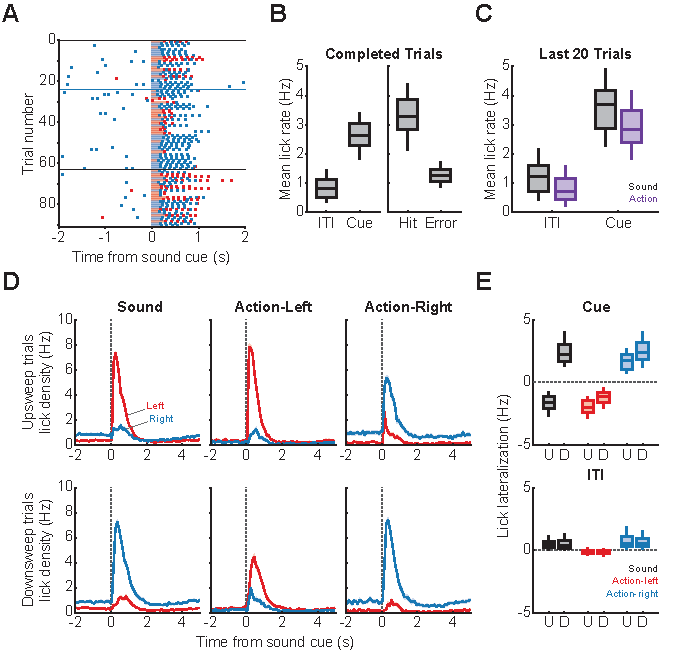
\includegraphics[width=11.4cm]{Figures/Chapter4/Fig2} 
\end{center}

\caption[Dependence of lick output on task structure]
{Dependence of lick output on the task structure. (A) Raster plot of individual lick times, aligned to cue onset during the first three blocks of an example session. Rows of the raster correspond to consecutive trials. The cue period of each trial is highlighted in pale red for upsweeps and pale blue for downsweeps, with red and blue tick marks representing left and right licks, respectively. Fine horizontal lines indicate the first trial of each rule block. The order of the blocks was sound--action-right--sound. (B) Mean lick rates for the 2 s periods before and after cue onset (ITI and Cue, respectively), estimated from all completed trials. Left, overall comparison of ITI and cue periods. Right, comparison of hit and error trials during the cue period. (C) Mean lick rates for the ITI and cue periods, presented separately for sound (black) and action trials (purple). (D) Lick density at the left (red) and right port (blue) across all sessions, calculated in 100 ms time bins surrounding cue onset. Data are plotted separately as the $\mathit{mean} \pm \mathit{SEM}$ for upsweep (top) and downsweep trials (bottom) within each block type. (E) Lick lateralization in upsweep (U) and downsweep trials (D) within each block type. Lick lateralization was calculated as the difference between the number of right and left licks during the 2 s before (bottom) and after cue onset (top) in each trial. Positive and negative values indicate a greater number of right and left licks, respectively. For C--E, analysis was restricted to the last twenty trials of each block: the period in which the accuracy criterion was met. For B--E, $N = 64$ sessions. Box plots in all figures represent quartiles 1--3 for each group. Whiskers indicate the 9th and 91st percentiles.}

\label{fig:Fig2}
\end{figure}


An important difference between sound and action trials is that a conditional mode of action selection \citep{mitz1991learning} is optimal under the sound rule; ie, only under the sound rule should choices depend on the identity of the sound cue. By contrast, the two action rules prescribe an unconditional mode of action selection that does not depend on cue identity. Therefore, in principle, correct choices could be made and even acted upon prior to cue onset in action trials, leading to rule-dependent differences in anticipatory licking.

To examine differences across rule types, we limited our analyses to the last twenty trials of each rule block---the period where at least 85$\%$  of choices were consistent with the corresponding rule. The mean pre-cue lick rate in action trials ($0.9 \pm 0.1$ Hz) was no greater than in sound trials ($1.2 \pm 0.1$ Hz; Fig. \ref{fig:Fig2}C). Moreover, the mean lick rate increased substantially upon cue onset in both sound and action trials (sound: $\Delta=2.4$ Hz, paired $t_{63} =28.7$, $p=\num{2e-38}$; action: $\Delta=2.1$ Hz, paired $t_{63}=29.7$, $p=\num{9e-39}$). Thus, the overall pattern of licking output was largely conserved across rule types, despite fundamental differences in their temporal constraints on action selection (Fig. \ref{fig:Fig2}D).

Sound, action-left, and action-right rules are defined by the instructive content of each sound cue. Specifically, upsweeps and downsweeps signify diverging targets during sound blocks (left vs. right), and convergent but opposing targets during action-left and action-right blocks. Thus, choices should depend on an interaction between cue identity and the current rule. However, the choice made on a given trial concerns only the initial lick following the sound cue. To examine the extent to which the overall pattern of directional licking was structured by the task, we calculated a measure of lick lateralization by subtracting the mean left-lick rate from the mean right-lick rate during the post-cue period of each trial. For example, in sound trials, lick lateralization was $-1.6 \pm 0.1$ Hz following an upsweep, and $2.5 \pm 0.1$ Hz following a downsweep.

We examined the dependence of this measure on cue identity, block-type, and their interaction with a 2-way repeated measures ANOVA  (Fig. \ref{fig:Fig2}E). Individual comparisons were made using Tukey’s post hoc test. As expected, this analysis revealed a significant dependence of lick lateralization on the interaction between block type and cue identity ($F_{2,126}=390$, $p=\num{6e-55}$). Specifically, lick lateralization following upsweeps versus downsweeps differed most during sound blocks ($\Delta=4.1$ Hz, $p=\num{1e-10}$). A much smaller difference was observed during action blocks (action-left: $\Delta=0.8$ Hz, $p=\num{1.1e-10}$; action-right: $\Delta=0.8$ Hz, $p=\num{1.1e-10}$). 

An identical analysis considering the pre-cue period revealed a small but significant difference in lick lateralization across rules (sound: $0.5 \pm 0.1$ Hz, action-left: $-0.1 \pm 0.0$ Hz, action-right: $0.7 \pm 0.1$ Hz; $F_{2,126} =100$, $p=\num{3e-27}$). As expected, neither the cue identity ($F_{1,63} =0.38$, $p=0.54$) nor the interaction of cue identity and block type ($F_{2,126} =1.6$, $p=\num{0.20}$) were significant predictors of lick lateralization during the pre-cue period.

\nnsub{Formal Measures of Task Performance}
Excluding the initial sound block, an average of $87 \pm 4$ trials were required to reach the accuracy criterion that triggered a rule switch (20 consecutive trials at $ \geq 85\%$ accuracy). Mean accuracy was slightly above criterion, at $86 \pm 0 \%$ during the final twenty trials of a rule block. Perseverative errors, defined as choices consistent with the previous rule but inconsistent with the current rule, were substantially more frequent than other errors. Specifically, $27 \pm 1$ perseverative errors and $3 \pm 0$ other errors were committed per block. The difference was significant in both sound ($\Delta=6$, paired $t_{63} =8.1$, $p=\num{2e-11}$) and action blocks ($\Delta=38$, paired $t_{63} =18.3$, $p=\num{6e-27}$).

\begin{figure}[htbp]

\begin{center}
\includegraphics[width=8.7cm]{Figures/Chapter4/Fig3} 
\end{center}

\caption[Formal measures of task performance]
{Formal measures of task performance. (A) Mean proportion of hits (green), perseverative errors (solid pink), other errors (dashed pink), and misses (gray) as a function of the number of trials from a rule switch across all sessions ($N=64$). Shading, SEM. (B) Box plots representing the mean proportion of hits (green) and preseverative errors (pink) for trials immediately preceding a rule switch (Pre) and for trials immediately following one (Post). Results are presented separately for switches from the sound rule to an action rule (left), and vice-versa (right). (C) Box plots representing the number of trials taken to reach criterion (left), and the number of perseverative errors committed (right), during sound (black) and action blocks (purple). All boxes represent quartiles 1--3; whiskers represent 9th and 91st percentiles.}

\label{fig:Fig3}
\end{figure}

As expected, accuracy dropped precipitously following a rule switch (\ref{fig:Fig3}A). The proportion of hits decreased from $98 \pm 1 \%$ in the trial before a rule switch, to $55 \pm 2 \%$ in the next trial (paired $t_{63} =16.8$, $p=\num{5e-25}$). This reduction in accuracy was mostly attributable to an increase in perseverative errors, which accounted for $0 \pm 0 \%$ of trials immediately preceding a rule switch and $35 \pm 2 \%$ of trials immediately following (paired $t_{63}=14.0$, $p=\num{4e-21}$). A much smaller increase was noted in the proportion of other errors ($\Delta=6\%$, paired $t_{63}=3.8$, $p=\num{3e-4}$) and misses ($\Delta=3\%$, paired $t_{63}=3.6$, $p=\num{7e-4}$). 

Results of this analysis are presented separately for switches from the sound rule to an action rule, and vice-versa, in Figure \ref{fig:Fig3}B. In both cases, the proportion of hits decreased substantially in the trial following a rule switch (sound-to-action: $\Delta=51\%$, paired $t_{63} =12.4$, $p=\num{1e-18}$; action-to-sound: $\Delta=35\%$, paired $t_{63} =8.8$, $p=\num{2e-12}$). Following a sound-to-action rule switch, the proportion of hits was indistinguishable from chance, at $46 \pm 4 \%$ ($t_{63}=1.0$, $p=0.30$; one-sample t-test for the null hypothesis, $H_0:\Delta=0.5$). In the case of action-to-sound rule switches, it remained significantly greater than chance, at $65 \pm 4 \%$ (one-sample $t_{63}=3.9$, $p=\num{2e-4}$). In both cases, the proportion of perseverative errors increased significantly (sound-to-action: $\Delta=39\%$, paired $t_{63} =10.1$, $p=\num{1e-14}$; action-to-sound: $\Delta=29\%$, paired $t_{63} =8.6$, $p=\num{3e-12}$).  

Although subjects were capable of adjusting sensorimotor decisions to both rule types, in general, they adapted more readily during action-to-sound rule transitions than the reverse (Fig. \ref{fig:Fig3}C). Substantially fewer trials were taken to reach the accuracy criterion in sound as compared to action blocks ($39 \pm 3$ vs. $126 \pm 6$; paired $t_{63} =13.2$, $p=\num{9e-20}$), and fewer perseverative errors were committed before the criterion was reached ($7 \pm 1$ vs. $43 \pm 2$; paired $t_{63} =14.0$, $p=\num{5e-21}$).

\nnsub{Task-Related Modulation of Neural Activity}

To gain insight into how distinct cell types in MFC contribute to the encoding of task-relevant information, we examined the recruitment patterns of GCaMP\textsuperscript{+} SST, VIP, PV, and PYR neurons both within and across trials. Example fields-of-view, along with cellular fluorescence time series obtained from each cell type, are shown in Figure \ref{fig:Fig4}A--H. 

\begin{figure}[htbp]

\begin{center}
\includegraphics[width=\textwidth]{Figures/Chapter4/Fig4} 
\end{center}

\caption[Task-related neural activity in SST, VIP, PV, and PYR neurons]
{Task-related neural activity in SST, VIP, PV, and PYR neurons. (A--D) Mean projections from example fields-of-view showing SST, VIP, PV, and PYR neurons, respectively. (E--H) Example $\frac{\Delta F}{F}$ traces from the sessions in A--D. Red and blue background shading correspond to the action-left and action-right rule, respectively. White background indicates periods governed by the sound rule. Vertical scale bar, 1 SD (I) Mean $\frac{\Delta F}{F}$ traces from the sessions shown in E--H, presented as a function of time relative to the sound cue. Grey lines represent the mean trace for each neuron across all completed trials, re-centered on the mean value obtained during the pre-cue period. The grand $\mathit{mean} \pm \mathit{SEM}$ across all cells is overlaid in color. (J) Proportion of task-modulated neurons within each cell type, across $N=$ 13, 19, 12, and 20 sessions from SST, VIP, PV, and PYR neurons, respectively.}

\label{fig:Fig4}
\end{figure}

All cellular fluorescence data are presented as $\frac{\Delta F}{F}$, which was calculated for each time point as $(F(t)-F_0(t))/F_0(t)$, where $F(t)$ is the mean of the raw fluorescence measured from the cell body at time $t$, and $F_0(t)$ is the 5th percentile of $F$ across a 10 min sliding window centered at time $t$. We focused on $\frac{\Delta F}{F}$ traces spanning the period from -2 to 5 s relative to each sound cue to examine time-dependent activity changes within each trial (Fig. \ref{fig:Fig4}I--J), and across trials that differed with respect to choice, outcome, and the current rule (Figs. \ref{fig:Fig5}--\ref{fig:Fig8}).

We quantified the sensitivity of SST, VIP, PV, and PYR populations to the temporal structure of the task by comparing the mean $\frac{\Delta F}{F}$ measured in the 2 s preceding each sound cue with that of the 5 s following it. Neurons showing a significant difference across these two epochs ($p<0.05$, Wilcoxon signed-rank test) were considered to have been modulated by the task. These included $78 \pm 5\%$ of PV, $77 \pm 3\%$ of SST, $63 \pm 3\%$ of VIP, and $56 \pm 4\%$ of PYR neurons (Fig. \ref{fig:Fig4}J). 

The proportion of task-modulated neurons varied significantly across cell types (Kruskal-Wallis $H_{3,60}=21.5$, $p=\num{8e-5}$). In particular, PYR populations included a significantly smaller proportion than either PV ($p=\num{9e-4}$, Tukey test) SST populations ($p=\num{1e-3}$, Tukey test). Tukey's post hoc test revealed no significant difference between PYR and VIP populations in this regard ($p=0.61$). PV and SST populations were likewise statistically indistinguishable ($p=1$). 

These results indicate task-related activity in substantial fractions of all four cell types. However, the activities of PV and SST neurons were preferentially modulated.

\nnsub{Modulation by Specific Task Variables}

Next, we examined the capacity of each cell type to encode specific behavioral variables crucial for task performance---namely, choices, outcomes, and rules. As an estimate for signal reliability in individual neurons, we calculated a modulation index based on the receiver operating characteristic (ROC) given by the responses of each neuron in varied trial conditions \citep{barlow1971responses,feierstein2006representation}. 

In the context of signal detection, the ROC captures the trade-off between sensitivity and specificity as detection parameters are varied. This relationship can be estimated empirically by taking the true positive rate (TPR) as a function of the false positive rate (FPR) at a series of detection thresholds. 

The area under the resulting curve (AUC) may serve as an unbiased scalar metric for signal discriminability. For example, if the neural activity levels associated with rewarded versus unrewarded trials yielded an AUC approaching 0 or 1, then an ideal observer could predict the trial outcome with an accuracy close to 100\% using these physiological data alone. By contrast, at an AUC of 0.5, chance-level accuracy would be expected. 

To assess choice, outcome, and rule signaling in each neuron, we calculated a modulation index $I(t) = 2(\mathit{AUC} - 0.5)$ as a function of time relative to the start of each trial, using cellular fluorescence traces obtained during subsets of trials that differed according to the behavioral variable of interest. For each variable, one subset of trials was arbitrarily chosen as the positive class ($\mathit{choice}=\mathit{left}$, $\mathit{outcome}=\mathit{reward}$, or $\mathit{rule}=\mathit{sound}$), and the remaining subset was assigned to the negative class ($\mathit{choice}=\mathit{right}$, $\mathit{outcome}=$ \emph{no reward}, or $\mathit{rule}=\mathit{action}$). Thus, $I(t)$ could range from -1 to 1, with positive and negative values reflecting a preference for positive and negative trials, respectively, and its magnitude $M(t)$ reflecting the signal reliability irrespective of preference.

\begin{figure}[htbp]

\begin{center}
\includegraphics[width=\textwidth]{Figures/Chapter4/Fig5}
\end{center}

\caption[Example cell modulated by choice, outcome, and rule context]
{Example cell modulated by choice, outcome, and rule context. (A) Mean $\frac{\Delta F}{F}$ traces from a single PYR neuron as a function of time relative to cue onset. Traces were averaged across trials in which the left (red) or right (blue) spout was chosen. Results are presented separately for trials governed by the sound (left) and action rule (right). Shading, bootstrapped 95\% confidence intervals. (B) Mean traces associated with rewarded (green) or unrewarded choices (pink) made in the current trial. Results are plotted as a function of time relative to cue onset in the current trial (left) and the trial immediately following the indicated outcome (right). (C) Mean traces from sound vs. action trials in which the same choice was made in response to the same sound cue and resulted in a reward. Left: upsweep-left trials governed by the sound (black) or action-left rule (red). Right: downsweep-right trials governed by the sound (black) or action-right rule (blue). (D--F) Example ROC curves calculated at the time points indicated by black arrowheads in A--C. Left trials, rewarded trials, and sound trials were arbitrarily assigned positive class membership for the analysis of choice, outcome, and rule signals, respectively. (G--I) The modulation index $I$, plotted as a function of time relative to cue onset for the full series of time points in A--C. For each time $t$, $I(t)$ was calculated from the area under the corresponding ROC curve (AUC) as $2*(\mathit{AUC}-0.5)$. The shaded intervals reflect the middle 95\% of $I_{0}(t)$, a null distribution generated by replicating the analysis using shuffled class labels.}

\label{fig:Fig5}
\end{figure}

As a summary for signal reliability within each cell type, we took two scalar estimates for each session: the mean modulation magnitude $\Bar{M}$, and the proportion of significantly modulated neurons $P$. $\Bar{M}$ was calculated as the grand mean of the modulation magnitude across all neurons during the first 5 s of the trial. $P$ was the proportion of neurons in which ${M}$ rose above chance for $\ge 1$ s within the same period. For example, Figure \ref{fig:Fig5} shows a PYR neuron that was significantly modulated by choice, outcome, and rule.

To summarize preference, we calculated the mean modulation index $\Bar{I}$ across neurons in each session, as well as the proportion of neurons with a significant preference for positive and negative trials (eg, $P_{\mathit{left}}$ and $P_{\mathit{right}}$). 

A Wilcoxon signed-rank test was used to compare $\Bar{M}$ or $\Bar{I}$ across sessions with the corresponding null results, and to compare $P$ with a corresponding set of false discovery rate estimates (FDR; see \hyperlink{methods_ROC}{Methods}). 

\nnsubsub{Choice-Related Modulation}

To examine choice-related modulation, we grouped $\frac{\Delta F}{F}$ traces according to whether the left or right spout was chosen in the corresponding trial. Sound and action trials were considered separately, and the analysis was limited to rewarded choices. 

The activity of all four cell types was modulated by choices made during the sound rule. In each case, modulation magnitude ${M}_{choice}(t)$ rose to significance within 250 ms of cue onset (Fig. \ref{fig:Fig6}A). The mean modulation magnitude $\Bar{M}_{\mathit{choice}}$ was significant for all four cell types, both in the current trial (SST: $\Bar{M}=0.14\pm0.01$, $W_{13}=1$, $p=\num{4e-4}$; VIP: $\Bar{M}=0.12\pm0.01$, $W_{19}=0$, $p=\num{1e-4}$; PV: $\Bar{M}=0.12\pm0.01$, $W_{12}=2$, $p=\num{0.001}$; PYR: $\Bar{M}=0.13\pm0.01$, $W_{20}=1$, $p=\num{1e-4}$), and the following trial (SST: $\Bar{M}=0.11\pm0.01$, $W_{13}=10$, $p=\num{0.01}$; VIP: $\Bar{M}=0.10\pm0.01$, $W_{19}=44$, $p=\num{0.04}$; PV: $\Bar{M}=0.10\pm0.01$, $W_{12}=9$, $p=\num{0.02}$; PYR: $\Bar{M}=0.11\pm0.01$, $W_{20}=46$, $p=\num{0.03}$).

\begin{figure}[htbp]

\begin{center}
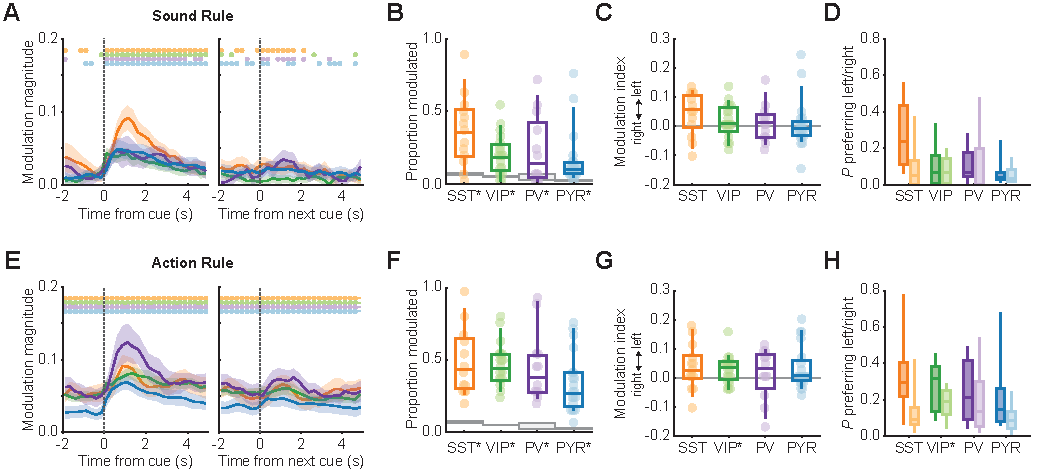
\includegraphics[width=\textwidth]{Figures/Chapter4/Fig6}
\end{center}

\caption[Choice-related modulation]
{Choice-related modulation. (A) Modulation magnitude $M$ with respect to the choice made in the current trial, plotted as a function of time relative to cue onset in the current trial (left) and the next trial (right). $M_{\mathit{choice}}(t)$ is presented as the difference from a null distribution obtained when the same analysis was conducted using shuffled choices. Line plots with shaded confidence intervals represent the $\mathit{mean} \pm \mathit{SEM}$ within SST (orange), VIP (green), PV (purple), and PYR populations (blue). Solid circles above indicate time bins where the corresponding cell type differed significantly from chance ($p<0.05$, Wilcoxon signed-rank test vs. shuffle). (B) The proportion of each cell population $P_{\mathit{choice}}$ that exhibited significant choice-related modulation in the current trial. (C) The mean modulation index $\bar{I}_{\mathit{choice}}$, calculated from the first 5 s of the current trial. (D) The proportion of each cell population exhibiting a significant preference for left ($P^+$) and right choices ($P^-)$, represented respectively in paired box plots to the left and right. (E--H) Same as A--C, for action blocks. For B--D and F--H, boxes indicate quartiles 1--3 and whiskers indicate the 9th and 91st percentiles of the empirical distribution. Values from individual sessions are represented in the beeswarm plots. Grey boxes represent quartiles 1 and 3 of the null distribution (visually indistinguishable from zero in C and G). Asterisks in B--C and F--G indicate significant differences from the null distribution for each cell type; in D and H, they indicate significant differences between $P^+$ and $P^-$ within each cell type; both were assessed at $\alpha = 0.05$, Wilcoxon signed-rank test. $N=$ 13 SST, 19 VIP, 12 PV, and 20 PYR populations.}

\label{fig:Fig6}
\end{figure}

Significant proportions of SST ($37\pm7\%$, $W_{13}=2$, $p=\num{7e-4}$), VIP ($20\pm3\%$, $W_{19}=7$, $p=\num{4e-4}$), PV ($23\pm7\%$, $W_{12}=6$, $p=\num{0.007}$), and PYR neurons ($17\pm4\%$, $W_{20}=0$, $p=\num{9e-5}$) were differentially recruited based on choice ($P_{\mathit{choice}}$; Fig. \ref{fig:Fig6}B). No significant differences in either $\Bar{M}_{\mathit{choice}}$ (Kruskal-Wallis $H_{3,60}=5.5$, $p=0.14$) or $P_{\mathit{choice}}$ ($H_{3,60}=5.6$, $p=0.16$) were found among cell types during the sound rule.

No substantial preference for left or right choices was evident at the population level for any of the cell types examined. In each case, the mean modulation index $\Bar{I}_{\mathit{choice}}$ did not differ significantly from chance ($p>0.05$ vs. shuffle; Fig. \ref{fig:Fig6}C). Moreover, the proportions of neurons exhibiting significant preference for left and right choices were approximately balanced within the VIP ($11\pm3\%$ vs. $9\pm2\%$, $W_{17}=66$, $p=0.62$), PV ($11\pm3\%$ vs. $12\pm6\%$, $W_{10}=25$, $p=0.85$), and PYR populations ($8\pm3\%$ vs. $8\pm3\%$, $W_{19}=88$, $p=0.78$) (Fig. \ref{fig:Fig6}D). Left-preferring neurons appeared to predominate within the SST population (left: $27\pm6\%$ vs. right: $10\pm4\%$), but the difference fell short of significance ($W_{12}=14.5$, $p=0.06$).

\paragraph{}
During the action rule, choices were reflected for the entirety of the trial in the activity of all four cell types. In each case, the modulation magnitude $M_{\mathit{choice}}(t)$ was significant throughout the 2 s leading up to the sound cue, and remained above chance in the 2 s before the next cue ($p>0.05$ vs. shuffle; Fig. \ref{fig:Fig6}E).\footnote{One limitation of our analysis is that the action rule reinforces repetition of a rewarded choice, leading to increased correlation between consecutive choices. Interpretation of $M_{\mathit{choice}}$ in this case remains somewhat ambiguous because the observed signals may reflect a combination of choice history and the current choice. For this reason, we only examined $\Bar{M}_{\mathit{choice}}$ in the current trial.} 

Accordingly, the mean modulation magnitude during action trials was significant for all cell types (SST: $\Bar{M}=0.14\pm0.01$, $W_{13}=0$, $p=\num{2e-4}$; VIP: $\Bar{M}=0.14\pm0.01$, $W_{19}=0$, $p=\num{1e-4}$; PV: $\Bar{M}=0.16\pm0.02$, $W_{12}=0$, $p=\num{5e-4}$; PYR: $\Bar{M}=0.11\pm0.01$, $W_{20}=0$, $p=\num{9e-5}$). A Kruskal-Wallis test revealed significant differences in $\Bar{M}_{\mathit{choice}}$ across cell types ($H_{3,60}=7.9$, $p=0.048$). However, no individual comparisons were significant (all $p>0.05$, Tukey test). 

Substantial proportions of all cell types were differentially recruited based on the choices made during action trials (SST: $48\pm7\%$, $W_{13}=0$, $p=\num{2e-4}$; VIP: $46\pm3\%$, $W_{19}=0$, $p=\num{1e-4}$; PV: $45\pm7\%$, $W_{12}=0$, $p=\num{5e-4}$; PYR: $34\pm5\%$, $W_{20}=0$, $p=\num{9e-5}$; Fig. \ref{fig:Fig6}F). No significant differences in $P_{\mathit{choice}}$ were found among cell types (Kruskal-Wallis $H_{3,60}=5.0$, $p=0.17$).

A significant overall preference for left or right choices was observed only among VIP neurons, which were preferentially active during trials where the left (contralateral) spout was chosen. The mean modulation index within VIP populations was significantly positive ($\Bar{I}=0.04\pm0.01$, $W_{19}=31$, $p=\num{0.01}$; Fig. \ref{fig:Fig6}G), and they contained a greater proportion of left- as compared to right-preferring neurons ($28\pm3\%$ vs. $18\pm2\%$, $W_{18}=40$, $p=0.048$; Fig. \ref{fig:Fig6}H). However, trends toward a contralateral population preference were also noted in SST ($P_{\mathit{left}}$: $34\pm7\%$ vs. $14\pm4\%$, $W_{11}=13$, $p=0.08$) and PYR populations ($24\pm5\%$ vs. $10\pm2\%$, $W_{20}=55$, $p=0.06$). No significant differences in $\Bar{I}$ were found between cell types (Kruskal-Wallis $H_{3,60}=0.4$, $p=0.95$). 

Comparisons of choice-related modulation across rule contexts revealed significantly stronger choice signals during action trials than during sound trials in all cell populations except SST. The difference was evident in both mean modulation magnitude (SST: $W_{13}=27$, $p=\num{0.22}$; VIP: $W_{19}=5$, $p=\num{3e-4}$; PV: $W_{12}=0$, $p=\num{5e-4}$; PYR: $W_{20}=23$, $p=\num{2e-3}$) and the proportion of each population exhibiting significant modulation (SST: $W_{13}=25$, $p=\num{0.17}$; VIP: $W_{19}=0$, $p=\num{1e-4}$; PV: $W_{12}=2$, $p=\num{1e-3}$; PYR: $W_{20}=18$, $p=\num{1e-3}$). 

Taken together, these results implicate all cell types examined in the representation of choices in M2. Choice signaling was evident during the current trial regardless of which rule was being enforced, but was more pronounced during the action rule. The summation of signals related to current and prior choices may partially account for this difference, due to the repetition of choices demanded by the action rule. During the sound rule, sustained choice-related activity was clearly evident in all four cell types, and persisted subsequent to the next sound cue. We also found limited evidence for preferential activity surrounding contralateral choices during action but not sound blocks---a trend that rose to significance only in VIP populations.       

\nnsubsub{Outcome-Related Modulation}
To investigate outcome-related modulation, we considered traces associated with rewarded vs. unrewarded choices, ie, hits vs. errors. We separately examined effects of the current trial outcome on neural activity in the current and subsequent trial. For the current trial, the previous outcome was held constant by limiting the analysis to $\frac{\Delta F}{F}$ traces preceded by a rewarded choice. Likewise, for the subsequent trial we held the corresponding outcome constant by focusing on traces associated with rewarded choices.

All cell types exhibited differential activity based on the trial outcome. Across cell types, modulation magnitude $M_{\mathit{outcome}}(t)$ was significant for all time bins $\ge 250$ ms following the sound cue, and the associated signals persisted well into the next trial ($p<0.05$, Wilcoxon signed-rank test; Fig. \ref{fig:Fig7}A). 
% \begin{SCfigure}[][htbp]
\begin{figure}[htp]

\begin{center}
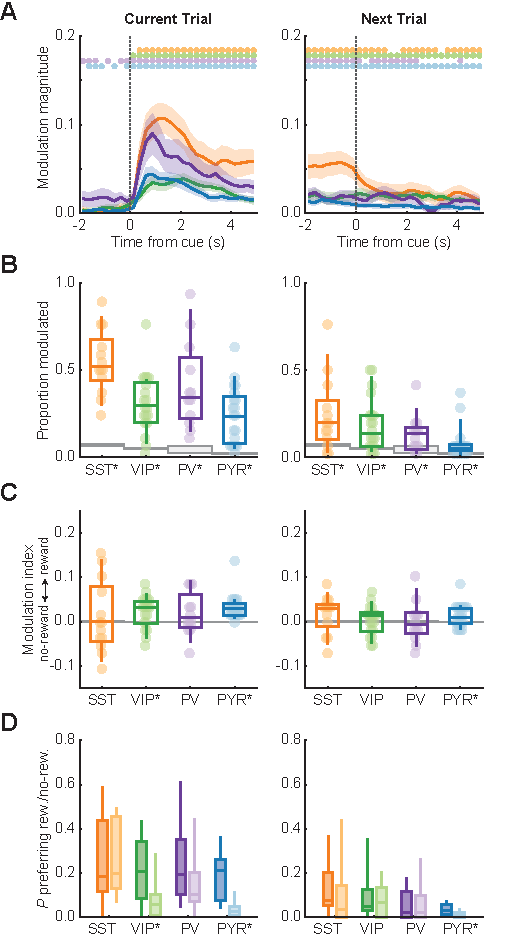
\includegraphics[width=8.7cm]{Figures/Chapter4/Fig7}
\end{center}

\caption[Outcome-related modulation]
{Outcome-related modulation. (A) Modulation magnitude $M$ with respect to the outcome of the current (left) and prior trial (right), plotted as in Figure \ref{fig:Fig6}A. Solid circles indicate time bins where $M_{\mathit{outcome}}(t)$ differed significantly from chance ($p<0.05$, Wilcoxon signed-rank test vs. shuffle) within SST (orange), VIP (green), PV (purple), and PYR populations (blue). (B) The proportion of each cell population, $P_{\mathit{outcome}}$, that exhibited significant modulation associated with the current (left) or prior outcome (right). (C) The mean modulation index $\bar{I}_{\mathit{outcome}}$ associated with the current (left) and prior outcome (right), calculated from the first 5 s of the trial. (D) The proportion of each cell population exhibiting a significant preference for rewarded ($P^+$; dark shading) and unrewarded choices ($P^-$; light shading), represented respectively in paired box plots. Left and right axes present the results with respect to the current and prior outcome, respectively. Asterisks in B--C indicate significant differences from the null distribution for each cell type; in D, they indicate significant differences between $P^+$ and $P^-$ within each cell type; both were assessed at $\alpha = 0.05$, Wilcoxon signed-rank test. $N=$ 13 SST, 19 VIP, 12 PV, and 20 PYR populations. All plots presented as in Figure \ref{fig:Fig6}.}

\label{fig:Fig7}
% \end{SCfigure}
\end{figure}

% {Outcome-related modulation. (A) Modulation magnitude $M$ with respect to the outcome of the current (left) and prior trial (right), plotted as a function of time relative to the sound cue. $M_{\mathit{outcome}}(t)$ is presented as the difference from a null distribution obtained when the same analysis was conducted using shuffled choices. Line plots with shaded confidence intervals represent the $\mathit{mean} \pm \mathit{SEM}$ within SST (orange), VIP (green), PV (purple), and PYR populations (blue). Solid circles above indicate time bins where $M_{\mathit{outcome}}(t)$ differed significantly from chance ($p<0.05$, Wilcoxon signed-rank test). (B) The proportion of each cell population, $P_{\mathit{outcome}}$, that exhibited significant modulation associated with the current (left) or prior outcome (right). (C) The mean modulation index $\bar{I}_{\mathit{outcome}}$ associated with the current (left) and prior outcome (right), calculated from the first 5 s of the trial. (D) The proportion of each cell population exhibiting a significant preference for rewarded ($P^+$) or unrewarded choices ($P^-$), represented respectively in paired box plots. Left and right axes present the results with respect to the current and prior outcome, respectively. Asterisks in B--C indicate significant differences from the null distribution for each cell type; in D, they indicate significant differences between $P^+$ and $P^-$ within each cell type; both were assessed at $\alpha = 0.05$, Wilcoxon signed-rank test. All plots presented as in Figure \ref{fig:Fig5}.}

The mean modulation magnitude $\Bar{M}_{\mathit{outcome}}$ was significant in all four cell types across the current trial (SST: $\Bar{M}=0.13\pm0.01$, $W_{13}=0$, $p=\num{2e-4}$; VIP: $\Bar{M}=0.09\pm0.00$, $W_{19}=0$, $p=\num{1e-4}$; PV: $\Bar{M}=0.11\pm0.01$, $W_{12}=0$, $p=\num{5e-4}$; PYR: $\Bar{M}=0.08\pm0.01$, $W_{20}=0$, $p=\num{9e-5}$) as well as the following trial (SST: $\Bar{M}=0.08\pm0.01$, $W_{13}=4$, $p=\num{0.002}$; VIP: $\Bar{M}=0.08\pm0.00$, $W_{19}=0$, $p=\num{1e-4}$; PV: $\Bar{M}=0.07\pm0.01$, $W_{12}=10$, $p=\num{0.02}$; PYR: $\Bar{M}=0.06\pm0.00$, $W_{20}=13$, $p=\num{6e-4}$). 

In both cases, differences in $\Bar{M}_{\mathit{outcome}}$ among cell types were significant (current trial: Kruskal-Wallis $H_{3,60}=13$, $p=0.005$; next trial: $H_{3,60}=12$, $p=0.007$), with SST neurons showing the strongest modulation, and PYR neurons showing the weakest. During the current trial, SST neurons differed significantly from VIP ($p=0.03$, Tukey test) and PYR neurons ($p=0.006$). In the next trial, SST and VIP neurons both differed significantly from PYR neurons ($p=0.02$ for both comparisons). 
%  with respect to the outcome of current (Kruskal-Wallis $H_{3,60}=13$, $p=0.005$) as well as prior choices ($H_{3,60}=12$, $p=0.007$). 

Modulation by the outcome of the most recent choice persisted throughout the last 2 s of the intertrial interval in all cell types, but was most pronounced in SST neurons (Fig. \ref{fig:Fig7}A, right). During this period, the mean modulation magnitude $\Bar{M}_{\mathit{outcome}}$ differed significantly among cell types (Kruskal-Wallis $H_{3,60}=10.9$, $p=0.01$), and was significantly greater in SST ($\Bar{M}=0.11\pm0.01$) as compared to either VIP ($0.08\pm0.01$, $p=0.03$, Tukey test) or PYR neurons ($\Bar{M}=0.06\pm0.00$, $p=0.01$). The difference from PV neurons fell short of significance ($\Bar{M}=0.08\pm0.01$, $p=0.15$). 
% (SST: $\Bar{M}=0.11\pm0.01$; PV: $\Bar{M}=0.08\pm0.01$; VIP: $0.08\pm0.01$; PYR: $\Bar{M}=0.06\pm0.00$)

A similar pattern was evident in the proportion of neurons modulated by outcome $P_{\mathit{outcome}}$ (Fig. \ref{fig:Fig7}B). For all cell types, the proportion exceeded chance in both the current trial (SST: $55\pm5\%$, $W_{13}=0$, $p=\num{2e-4}$; VIP: $30\pm4\%$, $W_{19}=1$, $p=\num{2e-4}$; PV: $41\pm7\%$, $W_{12}=0$, $p=\num{5e-4}$; PYR: $24\pm4\%$, $W_{20}=0$, $p=\num{9e-5}$) and the next trial (SST: $24\pm6\%$, $W_{13}=6$, $p=\num{0.003}$; VIP: $19\pm3\%$, $W_{19}=15$, $p=\num{0.001}$; PV: $13\pm3\%$, $W_{12}=8$, $p=\num{0.01}$; PYR: $7\pm2\%$, $W_{20}=19$, $p=\num{0.001}$). In the current trial, $P_{\mathit{outcome}}$ differed significantly among cell types (Kruskal-Wallis $H_{3,60}=15$, $p=0.002$), and SST populations included a significantly greater proportion of outcome-modulated neurons than either VIP (Tukey test: $p=0.01$) or PYR populations ($p=0.002$). However, significant differences among cell types did not persist into the next trial ($H_{3,60}=5.8949$, $p=0.12$).

% $P_{\mathit{outcome}}$ differed among cell types (Kruskal-Wallis $H_{3,60}=15$, $p=0.002$), and individual comparisons revealed a pattern similar to $\Bar{M}_{\mathit{outcome}}$. Namely, the proportion was greatest in SST populations and smallest in PYR populations. SST populations included a significantly greater proportion of outcome-modulated neurons than either VIP (Tukey test: $p=0.01$) or PYR populations ($p=0.002$). However, significant differences in $P_{\mathit{outcome}}$ did not persist into the next trial ($H_{3,60}=5.8949$, $p=0.12$).

An overall preference for rewarded choices was observed among PYR and VIP neurons (Fig. \ref{fig:Fig7}C). For both cell types, the mean modulation index $\Bar{I}_{\mathit{outcome}}$ was significantly positive (PYR: $\Bar{M}=0.032\pm0.006$, $W_{20}=1$, $p=\num{1e-4}$; VIP: $\Bar{M}=0.021\pm0.008$, $W_{19}=38$, $p=\num{0.02}$). PYR neurons also maintained a significantly positive $\Bar{I}_{\mathit{outcome}}$ into the next trial ($\Bar{M}=0.014\pm0.006$, $W_{20}=49$, $p=\num{0.04}$).

Furthermore, the proportion of neurons with preferential activity during rewarded trials outnumbered those preferring the absence of reward in both PYR ($20\pm3\%$ vs. $4\pm1\%$, $W_{20}=1$, $p=\num{1e-4}$) and VIP populations ($22\pm3\%$ vs. $9\pm2\%$, $W_{17}=28$, $p=\num{0.02}$; Fig. \ref{fig:Fig7}D). The proportions were approximately balanced within SST populations ($27\pm6\%$ vs. $28\pm5\%$, $W_{12}=39$, $p=\num{1}$), and did not differ significantly in PV populations ($25\pm6\%$ vs. $16\pm5\%$, $W_{11}=22$, $p=\num{0.37}$). In PYR populations, reward-preferring neurons continued to predominate into the next trial, although both proportions were greatly diminished ($5\pm2\%$ vs. $2\pm1\%$, $W_{17}=33.5$, $p=\num{0.04}$).

A Kruskal-Wallis test revealed no significant differences in $\Bar{I}_{\mathit{outcome}}$ among cell types, either in the current ($H_{3,60}=2.5$, $p=0.47$) or following trial ($H_{3,60}=3.3$, $p=0.34$). 

Collectively, these results indicate that trial outcomes were represented in the activity of all four cell types examined. Signals reflecting the outcome of the current choice rose to significance within 500 ms of the sound cue, consistent with the mean response time of $208 \pm 5$ ms in this set of experiments (IQR: 172--225 ms). In all cell types, the outcome signal persisted throughout the current trial, and well into the subsequent trial. SST activity exhibited the strongest modulation, with signals remaining notably elevated throughout the intertrial interval. Interestingly, SST populations contained roughly balanced proportions of neurons with preferential activity following rewarded and unrewarded choices, whereas PYR and VIP populations were more heavily recruited by reward.

\nnsubsub{Context-Related Modulation}
Finally, we examined modulation based on the rule context governing reinforcement in the current trial. For parity between sound and action trials, we only compared traces from trials where the same choice was made in response to the same sound cue (eg, upsweep-left-sound and upsweep-left-action trials). Additionally, we limited the analysis to rewarded choices made during the final twenty trials of each block---the period when choices were most consistent with the current rule.

Context-related modulation was observed in all cell types throughout the duration of the trial. In each case, $M_{\mathit{rule}}(t)$ was significant for all time bins during upsweep-left trials ($p<0.05$, Wilcoxon signed-rank test), and with the exception of SST neurons ($p<0.05$ in 15/20 bins), was also significant for all time bins during downsweep-right trials (Fig. \ref{fig:Fig8}A). In VIP, PV, and PYR neurons, $M_{\mathit{rule}}(t)$ was also significant for all time bins prior to the sound cue. SST neurons exhibited significant modulation throughout this period only during upsweep-left trials.

\begin{figure}[htbp]

\begin{center}
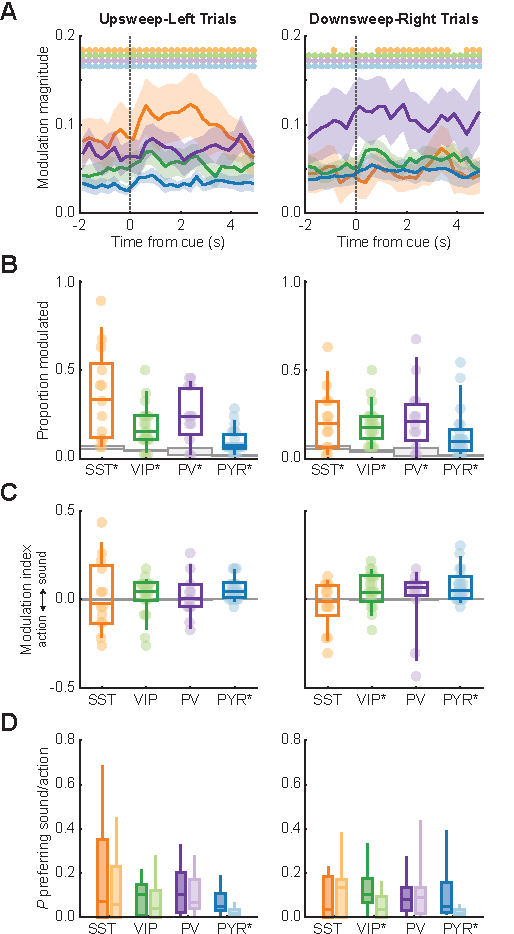
\includegraphics[width=8.7cm]{Figures/Chapter4/Fig8} 
\end{center}

\caption[Context-related modulation]
{Context-related modulation. Modulation by the current rule was examined under matched trial conditions: upsweep trials in which a left choice was rewarded (left), and downsweep trials in which a right choice was rewarded (right). (A) Modulation magnitude $M_{\mathit{rule}}(t)$ with respect to the rule governing the current trial (sound vs. action), plotted as in Figure \ref{fig:Fig6}A. Solid circles indicate time bins where $M_{\mathit{rule}}(t)$ differed significantly from chance ($p<0.05$, Wilcoxon signed-rank test vs. shuffle) within SST (orange), VIP (green), PV (purple), and PYR populations (blue). (B) The proportion of each cell population, $P_{\mathit{rule}}$, that exhibited significant modulation associated with the current rule. (C) The mean modulation index $\bar{I}_{\mathit{rule}}$, calculated from the first 5 s of the trial. (D) The proportion of each cell population exhibiting a significant preference for the sound ($P^+$; dark shading) and action rule ($P^-$; light shading), represented respectively in paired box plots. Asterisks in B--C indicate significant differences from the null distribution for each cell type; in D, they indicate significant differences between $P^+$ and $P^-$ within each cell type; both were assessed at $\alpha = 0.05$, Wilcoxon signed-rank test. $N=$ 13 SST, 19 VIP, 12 PV, and 20 PYR populations. All plots presented as in Figures \ref{fig:Fig6}--\ref{fig:Fig7}}

\label{fig:Fig8}
\end{figure}

% {Context-related modulation. Modulation by the current rule was examined under matched trial conditions: upsweep trials in which a left choice was rewarded (left), and downsweep trials in which a right choice was rewarded (right). (A) Modulation magnitude $M_{\mathit{rule}}(t)$ with respect to the rule governing the current trial (sound vs. action), plotted as a function of time relative to the sound cue.  Solid lines, mean; shading, SEM. Solid circles above indicate time bins where $M_{\mathit{rule}}(t)$ differed significantly from chance ($p<0.05$, Wilcoxon signed-rank test). (B) The proportion of each cell population, $P_{\mathit{rule}}$, that exhibited significant modulation associated with the current rule. (C) The mean modulation index $\bar{I}_{\mathit{rule}}$, calculated from the first 5 s of the trial. (D) The proportion of each cell population exhibiting a significant preference for the sound ($P^+$; dark shading) and action rule ($P^-$; light shading), represented respectively in paired box plots. Asterisks in B--C indicate significant differences from the null distribution for each cell type; in D, they indicate significant differences between $P^+$ and $P^-$ within each cell type; both were assessed at $\alpha = 0.05$, Wilcoxon signed-rank test. All plots presented as in Figures \ref{fig:Fig5}--\ref{fig:Fig6}}

Nevertheless, $\Bar{M}_{\mathit{rule}}$ was significant within all cell types during both upsweep-left (SST: $\Bar{M}=0.27\pm0.03$, $W_{13}=2$, $p=\num{7e-4}$; VIP: $\Bar{M}=0.21\pm0.02$, $W_{19}=5$, $p=\num{3e-4}$; PV: $\Bar{M}=0.23\pm0.02$, $W_{12}=0$, $p=\num{5e-4}$; PYR: $\Bar{M}=0.20\pm0.01$, $W_{20}=0$, $p=\num{9e-5}$) and downsweep-right trials (SST: $\Bar{M}=0.20\pm0.02$, $W_{13}=8$, $p=\num{0.006}$; VIP: $\Bar{M}=0.22\pm0.01$, $W_{19}=0$, $p=\num{1e-4}$; PV: $\Bar{M}=0.26\pm0.04$, $W_{12}=0$, $p=\num{5e-4}$; PYR: $\Bar{M}=0.20\pm0.01$, $W_{20}=0$, $p=\num{9e-5}$). 

Substantial fractions of each cell population were differentially recruited based on the rule context (Fig. \ref{fig:Fig8}B). For each cell type, the proportion of neurons $P_{\mathit{rule}}$ significantly modulated by the current rule exceeded chance in both sets of trials examined (upsweep-left---SST: $35\pm7\%$, $W_{13}=2$, $p=\num{7e-4}$; VIP: $18\pm3\%$, $W_{19}=8$, $p=\num{5e-4}$; PV: $24\pm4\%$, $W_{12}=3$, $p=\num{0.002}$; PYR: $10\pm2\%$, $W_{20}=0$, $p=\num{9e-5}$; downsweep-right---SST: $22\pm5\%$, $W_{13}=8$, $p=\num{0.006}$; VIP: $19\pm3\%$, $W_{19}=2$, $p=\num{2e-4}$; PV: $23\pm6\%$, $W_{12}=3$, $p=\num{0.002}$; PYR: $14\pm3\%$, $W_{20}=0$, $p=\num{9e-5}$). 

A Kruskal-Wallis test revealed no significant differences in $\bar{M}_{\mathit{rule}}$ among cell types (Kruskal-Wallis $H_{3,60}=6.4$, $p=0.09$ for both sets of trials). However, $P_{\mathit{rule}}$ differed significantly during upsweep-left trials ($H_{3,60}=9.0$, $p=0.03$). In particular, SST populations included a significantly greater proportion of rule-modulated neurons than did PYR populations ($p=0.045$). The proportion in PV populations also tended to exceed PYR populations, but the difference did not reach significance ($p=0.09$). No significant differences in $P_{\mathit{rule}}$ could be observed between cell types during downsweep-right trials ($H_{3,60}=2.6$, $p=0.46$).

To examine whether neural activity was affected by the interaction of choices with the rule context in which they were made, we also compared $\bar{M}_{\mathit{rule}}$ and $P_{\mathit{rule}}$ estimated from upsweep-left versus downsweep-right trials within each cell type. No significant differences were found across the two trial subsets (all $p>0.05$, Wilcoxon signed-rank test), although a trend was observed in SST populations ($W_{13}=19$, $p=0.07$).

A consistent preference for one rule context over the other was found only within PYR populations, which were preferentially active during the sound rule (Fig. \ref{fig:Fig8}C--D). Across PYR neurons, the mean modulation index $\bar{I}_{rule}$ was significantly positive during both upsweep-left ($\bar{I}=0.06\pm0.01$, $W_{20}=14$, $p=\num{7e-4}$) and downsweep-right trials ($\bar{I}=0.08\pm0.02$, $W_{20}=16$, $p=\num{9e-4}$). In both cases, sound-preferring neurons made up a comparatively greater proportion of the population than those preferring the action rule (upsweep-left: $7\pm1\%$ vs. $2\pm1\%$, $W_{20}=31$, $p=\num{0.006}$; downsweep-right: $11\pm3\%$ vs. $2\pm0\%$, $W_{18}=23$, $p=\num{0.006}$). 

Preference for the sound rule was also evident in the VIP population. In downsweep-right trials, $\bar{I}_{rule}$ was significantly positive ($\bar{I}=0.05\pm0.02$, $W_{19}=41$, $p=0.03$), and a significantly greater proportion of the population was preferentially active during sound as compared to action trials ($14\pm3\%$ vs. $5\pm2\%$, $W_{18}=38.5$, $p=0.04$). However, in upsweep-left trials, $\bar{I}_{rule}$ did not differ significantly from chance ($\bar{I}=0.02\pm0.02$, $W_{19}=58$, $p=0.14$), and the proportions of the VIP population preferring sound and action rules were approximately balanced, at $10\pm2\%$ and $9\pm3\%$, respectively ($W_{16}=51$, $p=0.38$). Furthermore, $\bar{I}_{rule}$ did not differ significantly between upsweep-left and downsweep-right trials (median $\Delta=0.02$, $W_{19}=69$, $p=0.30$), providing little evidence for a choice-rule interaction effect.

No significant differences in $\bar{I}_{rule}$ were detected among cell types (upsweep-left: $H_{3,60}=4.3$, $p=0.23$; downsweep-right: $H_{3,60}=1.7$, $p=0.64$).

These results indicate that, similar to choices and outcomes, the current rule context was reflected in the activities of SST, VIP, PV, and PYR populations. In most cases, rule signals were evident for the entire period between -2 and 5 s from cue onset. The strength of rule signals was similar among cell types, and differed only during trials where the contralateral spout was chosen. During these trials, neurons modulated by rule context were relatively more frequent in SST as compared to PYR populations. An overall preference for one rule context over the other was found only within the PYR population, which was more heavily recruited during the sound rule as compared to the action rule.             
% As median difference in proportion (save in case requested). Use this format for first reference: $P_{\mathit{left}}-P_{\mathit{right}}$: median $\Delta=15\%$
% PYR upsweep-left: median $\Delta=3\%$, $W_{20}=179$, $p=\num{0.006}$; downsweep-right: median $\Delta=3\%$, $W_{20}=148$, $p=\num{0.006}$). VIP downsweep-right: median $\Delta=5\%$, $W=133$, $p=0.04$; upsweep-left median $\Delta=6\%$, $W_{19}=85$, $p=0.38$; (upsweep-left--SST: median $\Delta=0\%$, $W_{13}=43.5$, $p=\num{0.75}$; PV: median $\Delta=0\%$, $W_{12}=31$, $p=\num{0.77}$; downsweep-right--SST: median $\Delta=3\%$, $W_{13}=32$, $p=\num{0.61}$; PV: median $\Delta=3\%$, $W_{12}=24.5$, $p=\num{0.84}$)

%Summary: 
% Try to bring back *task-related information coding*
% Context-dependent activity in interneurons vs. PYR: inconclusive, but some evidence for preferential modulation of interneurons.
% Preference: PYR & VIP, although the results were less conclusive for VIP (interaction unlikely: I(rule_SL vs rule_SR): median diff=0.02, W(19)=69, p=0.30).

% Discussion
\newpage
\nnsec{Discussion}

We used cell type-specific Ca$^{2+}$ imaging during a rule switching task to study the neural correlates of adaptive sensorimotor behavior in the MFC. Task-related activity was evident in the majority of SST, VIP, PV, and PYR neurons. To measure the reliability of single-unit responses to specific task variables, we calculated a modulation index based on the receiver operating characteristic. Substantial proportions of each cell population carried signals related to choices, outcomes, and the current rule context. These results provide insight on the question of how task representations are distributed among cell types within a cortical region known to function in goal-directed sensorimotor behaviors.

\paragraph{} Based on their subcellular postsynaptic targets, specific classes of GABAergic interneurons are suitably positioned to regulate the flow of activity through cortical networks \citep{kepecs2014interneuron}. Namely, SST+ interneurons preferentially target the dendrites of pyramidal cells, and PV+ interneurons preferentially target their cell body and proximal axon. These subcellular anatomical features correspond to the excitatory inputs and outputs, respectively, of the principal cells which may project within or outside of the local microcircuit. More broadly, SST and PV mediated inhibition, respectively, might serve to route the information flowing into and out of the processing units within MFC. In contrast to other inhibitory cell-types, VIP+ interneurons almost solely target other interneurons, and make particularly strong synapses on SST neurons. Thus, VIP cells appear to specialize in disinhibition \citep{letzkus2011disinhibitory,pi13,karnani2016opening}, and in particular may disinhibit the dendrites of pyramidal neurons through their suppression of SST activity.  

Despite striking differences in synaptic connectivity, all of the inhibitory cell types imaged in our experiments carried signals for the behavioral variables most important for task performance---namely, choices, outcomes, and the rule context governing reinforcement in the current trial. These results suggest that the specialized forms of inhibition that distinguish these populations may all function in the processing of diverse task representations in the MFC. 

Choice signaling was clearly evident in SST, VIP, PV, and PYR neurons regardless of which rule was being enforced, but was more pronounced during action trials. The summation of activity related to current and prior choices may partially account for this difference, due to the repetition of choices demanded by the action rule. We examined the persistence of choice-related signaling during the sound rule, and found that it lasted well into the next trial in all four cell types. We also found limited evidence for preferential activity surrounding contralateral choices during action but not sound blocks---a trend that rose to significance only in VIP populations. Some degree of choice preference would be consistent with previous results of unilateral MFC inactivation, which induced an ipsilateral choice bias during sensorimotor behavior specifically in the absence of instructive spatial cues \citep{erlich2011cortical,erlich2015distinct,hanks2015distinct}. Endogenous differences in the interhemispheric balance of MFC activity may in this case reflect a goal-directed choice bias, which would be one solution to the stimulus-response-outcome contingencies of the action rule.

Trial outcomes were also represented in the activity of all four cell types. In each case, outcome signals persisted throughout the current trial and well into the subsequent trial. SST activity exhibited the strongest and most sustained modulation, with signals remaining notably elevated throughout the intertrial interval. SST populations also included the largest percentage of outcome-responsive neurons. Interestingly, they contained roughly balanced proportions of neurons with preferential activity following rewarded and unrewarded choices. PYR and VIP populations were more heavily recruited following rewarded choices. This result is in agreement with a previous study where reinforcement was found to elicit VIP activity in the primary auditory cortex (A1) during an auditory go/no-go task \citep{pi13}. The same study found that VIP stimulation could indirectly recruit pyramidal neurons in A1 or mPFC through disinhibition.  

Similar to choices and outcomes, the current rule context was also reflected in the activities of all four cell types. In most cases, rule signals were evident for the entire duration of the trial. The proportion of neurons exhibiting differential recruitment across rules was similar among cell types, and differed only during trials where the contralateral spout was chosen. During these trials, a greater proportion of significantly modulated neurons was found in SST as compared to PYR populations. An overall preference for one rule context over the other was found only within the PYR population, which was more heavily recruited during the sound rule as compared to the action rule. We have previously found that bilateral pharmacological inactivation in MFC caused context-dependent effects on behavioral adjustment following a rule switch---namely, adjustment was disrupted under the sound rule and enhanced under the action rule \citep{siniscalchi2016fast}. Preferential PYR activity during the sound rule fits well with idea that MFC should exert greater control over behavior in contexts that require the engagement of arbitrary sensorimotor associations. 

\paragraph{}One important limitation of our approach regards the temporal resolution of the $\frac{\Delta F}{F}$ signals measured in our experiments. The temporal resolution of two-photon Ca$^{2+}$ imaging data is bounded by a number of factors including the sampling rate (which may be dependent on scanner type), the response kinetics of the calcium indicator, and the time course of changes in cytosolic Ca$^{2+}$ concentration caused by action potentials. Scanning methods trade off sampling rate for a greater number of pixels per frame. In order to record from a large number of neurons simultaneously and at cellular resolution, our time-lapse imaging data were obtained at $\sim3.6$ Hz using galvanometric scanners. These data were well-suited to compare signals resulting from changes in firing rates on the scale of hundreds of ms. However, more rapid fluctuations that could be of physiological importance may have been attenuated. Additionally, the intrinsic time course of changes in cytosolic free Ca$^{2+}$ concentration is dependent on subcellular compartmentalization, the compliment of membrane ion channels, calcium release from internal stores, and cytosolic calcium buffers \citep{higley2008calcium,higley2012calcium} all of which can vary by cell type \citep{lee2000differences}.

\paragraph{} During the rule switching task, mice were able to adjust their behavior to meet the abrupt shifts in the contingencies between sensory cues, actions, and outcomes that were associated with transitions between rule contexts.  However, adjustment to the sound rule generally required far fewer trials than the action rule ($39 \pm 3$ vs. $126 \pm 6$; Fig. \ref{fig:Fig3}). This result conflicts with our previous study using an almost identical task, in which subjects required $\sim$ 40 trials to complete sound or action blocks \citep{siniscalchi2016fast}. Two differences in the structure of the earlier version of the task may account for this discrepancy: (1) it included a 500 ms grace period following each sound cue, during which time any recorded responses would not affect the trial outcome, and (2) the intertrial interval (ITI) was set at a constant duration of 7 s between sound cues. In the present study, a choice was made with the first lick following cue onset, and the random ITI (5-16 s, drawn from a truncated exponential distribution with a mean of 8 s) precluded accurate prediction of the next cue onset time. Although unexpected, the results of this manipulation suggest that the ability to inhibit well-learned stimulus-response associations may be disrupted when choices are offered at unpredictable time intervals.    

\paragraph{} Reversible inactivation experiments have implicated the MFC in lateralized decisions informed by either short-term memory \citep{erlich2011cortical,guo2014flow,kopec2015cortical} or the gradual accumulation of sensory evidence \citep{erlich2015distinct,hanks2015distinct}. Additionally, our own recent study found that bilateral MFC inactivation during the rule switching task impaired performance only during adjustment to the sound rule, when the task required the use of learned sensorimotor associations \citep{siniscalchi2016fast}. Using two-photon Ca$^{2+}$ imaging, we also observed transitions in population activity in MFC as the mice adjusted their behavior following a rule switch. Transitions occurred earlier and were more abrupt during the sound rule as compared to the action rule, despite a similar time course of behavioral adjustment. Taken together, these results may suggest that the use of antecedent conditions to guide lateralized action selection comprises a critical function of MFC in decision making.

The local circuit mechanisms within MFC that may realize this cognitive-level function remain unclear. More fundamentally, knowledge of the relationship between afferent and efferent information content may be needed to define the specific computations performed. Further investigations will be necessary to illuminate the precise role of MFC in sensorimotor decision-making---in part by determining how task-related information carried by neuronal activity is transformed within the local network. 

% Materials & Methods
%\newpage

% TEXT OF MATERIALS & METHODS 

\nnsec{Materials and Methods}
\label{sec:methods} %Label for \autoref, etc.

\newcommand{\tg}[1]{\textsuperscript{\textit{#1}}}

\subsection*{Experimental Subjects}
Experimental subjects ($N=18$) were adult male transgenic mice from a C57BL/6J genetic background (Supplementary Table \ref{tab:expTable}). All mice were hemizygous hybrids of the following strains purchased from the Jackson Laboratory (Bar Harbor, ME): Sst\tg{tm2.1(cre)Zjh}/J (\emph{SST-cre}; stock no. 013044), Vip\tg{tm1(cre)Zjh}/J (\emph{VIP-cre}; stock no. 010908), B6.129P2-Pvalb\tg{tm1(cre)Arbr}/J (\emph{PV-cre}; stock no. 017320), or B6.Cg-Gt(ROSA)26Sor\tg{tm9(CAG-tdTomato)Hze}/J (\emph{flex-tdTomato}; stock no. 007909). Six subjects were bred from B6.Cg-Igs7\tg{tm148.1(tetO-GCaMP6f,CAG-tTA2)Hze}/J mice (\emph{Ai148}; Allen Institute). Specifically, a total of seven \emph{PV-cre;flex-tdTomato mice}, five \emph{SST-cre;flex-tdTomato mice}, five \emph{VIP-cre;Ai148} mice, and one \emph{PV-cre;Ai148} mouse were used for our experiments.


% Six subjects were bred from B6.Cg-Igs7\tg{tm148.1(tetO-GCaMP6f,CAG-tTA2)Hze}/J mice (\emph{Ai148}; \cite{daigle18}) provided by Hongkui Zeng (Allen Institute, Seattle, WA).

Mice were housed in a dedicated facility administered by the Yale Animal Resource Center. Five littermates were kept together per cage, supplemented with an igloo and cotton nesting material. Room lights were turned on from 7 am until 7 pm. Training and experiments were conducted outside of the facility between the hours of 10 am and 6 pm. All experimental procedures were approved by the Institutional Animal Care and Use Committee of Yale University.


\subsection*{Behavioral Apparatus}

All imaging data were collected while mice engaged in a sound-guided decision making task under head-fixation. The behavioral apparatus was nearly identical to that used in earlier studies \citep{siniscalchi2016fast,siniscalchi2019enhanced}. 

Briefly, the subject was placed under a two-photon microscope, resting in a modified stainless steel tube with a 1.25 inch inside diameter. Head-fixation was achieved using a custom stainless steel headplate and headplate holder (eMachineShop) secured to an anodized aluminum breadboard (MB4, Thorlabs) that could be bolted to an optical table holding the microscope. 

Sound cues were played through a set of PC speakers (S120; Logitech), and calibrated to a peak amplitude of $\sim 85$ \si{\dB}. 

Two 20-guage stainless steel dispensing tips (CML Supplies) placed on either side of the subject's mouth were used as lick spouts for the delivery of water rewards. The spouts were mounted in a 3D-printed plastic adapter to a set of optical components that allowed positional adjustment in three dimensions (height-adjustable post and dovetail rails; Thorlabs). A battery-operated lick detection circuit
\citep{slotnick2009simple} was connected to each spout with soldered wire leads. Signals from the detector, which supplies 5 \si{\V} upon contact with the tongue, were digitized with a USB data acquisition device (USB-201; Measurement
Computing) and recorded on a desktop PC. 

Water rewards ($\sim$ 2 \si{\uL}) were gravity-fed to each spout through Tygon tubing (Cole-Parmer) equipped with a solenoid valve (MB202VA30L204; Gems Sensors) controlled by TTL pulses from a second USB-201. 

The entire task structure---including sound cue playback, lick detection, and reward delivery---was automated using custom scripts written for Presentation
(Neurobehavioral Systems, Inc.). The computer code and all details of the behavioral apparatus can be found at \url{www.github.com/Kwan-Lab}.

\subsection*{Rule Switching Task}

The task consisted of a set of trials in which subjects could choose between two stainless steel water spouts placed on either side of the mouth, only one of which (the target) would provide a water reward on a given trial. A sound cue played at the start of each trial indicated the target side. The cues were repeated logarithmic chirps of 500 ms duration, with starting and ending frequencies of either 5 and 15 kHz (upsweeps), or 15 and 5 kHz (downsweeps), respectively. 

Each trial was governed by one of three rules---\emph{sound}, \emph{action-left}, or \emph{action-right}---that defined the target water spout associated with each sound cue. In the sound rule, upsweeps indicated a left target, and downsweeps indicated a right target. In the action-left rule, the target on every trial was the left spout, regardless of whether upsweeps or downsweeps were presented. Conversely, under the action-right rule, the right spout was always the target, irrespective of the sound cue. 
The sound cue was terminated by the first lick following cue onset, up to a maximum of 2 s. If the target spout was chosen (a hit), subjects were immediately rewarded with $\sim$ 2 \si{\uL} of water. Choosing the non-target spout (an error) resulted in playback of a mild white noise sound. The next sound cue was presented after a random interval drawn from a truncated exponential distribution (mean: 8 s, range: 5--16 s). 

Sessions were structured into alternating blocks of sound and action trials, and action blocks alternated between the action-left and action-right rule. The first action rule was drawn randomly. Each rule was enforced for at least 20 trials at a time, with the exact number of trials subject to a performance criterion: after 20 consecutive trials with $\geq 85\%$ accuracy, a new rule block would begin on the next trial. New trials were generated until the subject failed to respond (missed) for twenty consecutive trials.

To prepare for the rule-switching task, subjects were first trained for several weeks on trials governed by the sound rule. Training was conducted once daily for 6 d/wk, starting $>7$ d following the completion of surgery. On non-training days, subjects were administered water \emph{ad libitum} for 15 min in their home cages. Body weight was measured before and after each daily training session to guard against dehydration, and all mice maintained $>85\%$ of their starting body weight over the course of study. 
Full details of the training procedure can be found in \cite{siniscalchi2016fast} or \cite{siniscalchi2019enhanced}, with two exceptions. Our previous studies 1) included a 500 ms "grace period" following the sound cue, during which time any recorded responses would not affect the trial outcome, and 2) used a fixed intertrial interval of 7 s following cue offset. All other details of the behavioral protocols were conserved. 

\subsection*{Cell Type Specific Imaging}
We used two-photon calcium imaging to monitor neural activity at cellular resolution while mice participated in the rule switching task. To separately measure the activity of somatostatin- (SST; $N=290$ cells from five mice), parvalbumin- (PV; $N=263$ cells from three mice), and vasointestinal peptide-expressing interneurons (VIP; $N=488$ cells from five mice), as well as CamKIIa-expressing excitatory neurons (PYR; $N=3952$ cells from five mice), we took three different approaches which have all been validated in earlier studies.

To image the activity of SST and PV neurons, a cyclic recombinase- (cre) dependent adeno-associated virus encoding GCaMP6s (AAV1-hSyn-Flex-GCaMP6s-WPRE-SV40, Penn Vector Core) was injected intracranially in hybrid reporter mice (five SST::tdTomato and two PV::tdTomato) that express both cre and the orange fluorescent protein, tdTomato, selectively in the cell-type of interest \citep{taniguchi11, ali20}. Neuronal expression of tdTomato was aimed at providing a frame-by-frame anatomical reference channel to be used later for movement correction of data from the activity-dependent (GCaMP) channel. 

To monitor VIP and PV neurons, we bred VIP::GCaMP6f and PV::GCaMP6f hybrid reporter mice (five mice and one mouse, respectively), which selectively express GCaMP6f in the cell-type of interest \citep{daigle18,devries20}. 
To monitor pyramidal neurons, five PV-cre::tdTomato mice were injected intracranially with an AAV encoding GCaMP6f under control of the CaMKII-promoter (AAV1-CaMKII-GCaMP6f-WPRE-SV40, Penn Vector Core; \cite{kuchibhotla17,ali20}).

\subsubsection*{Intracranial Injections and Cranial Window Implantation}
Subjects were treated preoperatively with analgesic and anti-inflammatory drugs (carprofen, 5 mg/kg, SC, \#024751, Butler Animal Health; and dexamethasone, 3 mg/kg, SC, Dexaject SP, \#002459, Henry Schein Animal Health). Anesthesia was induced with 2\% isoflurane in oxygen, and then gradually reduced to 1--1.5\% for the remainder of the procedure. A water-circulating heating pad (Gaymar Stryker) was placed under the animal’s body, and maintained at 38\si{\celsius}.

After stabilizing the head in a stereotaxic frame with ear bars (David Kopf Instruments), the scalp was shaven and cleaned with Betadine (Perdue Products L.P.). The surface of the skull was then exposed through a midsagittal incision extending from the interaural line to the level of the orbits. The periosteum was removed, and the skull cleaned, by scrubbing briefly with 3\% hydrogen peroxide on a cotton swab. All contacted tissue was then rinsed immediately with artificial cerebrospinal fluid (aCSF; in mM: 5 KCl, 5 HEPES, 135 NaCl, 1 MgCl$_2$, 1.8 CaCl$_2$; pH 7.3).

A 3-mm-diameter circular craniotomy, centered approximately over the target location in M2 (AP, $\mathit{bregma}+1.5$ mm; ML, $\mathit{bregma}-0.5$ mm), was made using a 400-\si{\um}-diameter spherical bur attached to a Foredom dental drill. The circumscribed section of skull was then carefully removed with fine forceps to expose the dura. A small cube of Gelfoam (McKesson), presaturated with aCSF, was immediately applied to ensure hemostasis. Several additional cubes of saturated Gelfoam were used to gently cleanse the dural surface of any debris.

For procedures requiring intracranial AAV injections, a fine-tipped glass micropipette was secured to a microinjection system (Nanoject II, Drummond) and front-filled with ~1.5 \si{\uL} of the viral suspension. All viruses were stored as frozen aliquots, and diluted to approximately 1012 genome copies per mL in PBS prior to injection. Four injections were made, forming a 200-\si{\um}-wide square centered on the target location. Approximately 46 nL were injected into each site, at a depth of 400 \si{\um} below the dura. After the last injection, the dura was cleaned thoroughly with saturated Gelfoam.

A glass window implant was then fit to the craniotomy and glued to the surrounding skull surface. The implant consisted of five concentric, \#1 thickness, circular glass coverslips (Warner Instruments) joined with an optical adhesive (NOA 61, Norland). The superficial layer was wider than the remaining layers (4- vs. 3-mm-diameter), to form a lip that could be attached to the skull. Prior to implantation, the window was swabbed thoroughly with 90\% ethanol and then rinsed with aCSF. After flooding the craniotomy with aCSF, the implant was lowered into place and secured with a high-viscosity adhesive (Loctite 454). After allowing ~10 min for the adhesive to cure, a custom-made stainless steel headplate (eMachineShop.com) was cemented to the skull with C\&B Metabond (Parkell). Care was taken to cover any exposed bone.

Subjects were treated post-operatively with carprofen (5 mg/kg, SC), diluted to 0.17 mg/mL in 0.9\% preservative-free saline (Hospira) for fluid support. The treatment was repeated twice daily for three days following the surgery, along with a daily injection of dexamethasone (3 mg/kg, SC). At least one full week was allowed for recovery prior to behavioral training.

\subsubsection*{Two-Photon Microscopy}
To image neural activity at cellular resolution in vivo, an ultrafast laser beam (Chameleon Ultra II, Coherent) was focused on the brain tissue through a water immersion objective (XLUMPLFLN, $20\times$/0.95 NA; Olympus) attached to a Movable Objective Microscope (Sutter Instrument). Ultrasound gel (\#9004352SM, Henry Schein) was applied to the cranial window as an immersion medium, to prevent a gradual image degradation observed in earlier experiments due to evaporation.
Excitation power after the objective was adjusted using a Pockels cell (350-80-LA-
02; Conoptics), up to a maximum of 100 mW. Emitted fluorescence was split between two channels and bandpass filtered at center wavelengths of 525 nm (GCaMP6) and 605 nm (tdTomato) prior to collection by a set of GaAsP photomultiplier tubes (H7422P-40MOD; Hamamatsu). Excitation wavelength was set to 1020--1050 nm for most experiments, in order to optimize the GCaMP6:tdTomato emission ratio. For single-channel GCaMP6 imaging, an excitation wavelength of 940 nm was used.

Image acquisition was controlled by the ScanImage package for MATLAB (The MathWorks) \citep{pologruto03}. Time-lapse images of the field-of-view (FOV) were acquired using a bidirectional raster scan at 1kHz. Each imaging frame contained $256 \times 256$ pixels, for a nominal frame rate of 3.62 Hz including flyback time. Frames from each behavioral trial were saved separately in multi-page tagged image file format (TIFF). Imaging and behavioral data were synchronized by assigning an external trigger in ScanImage to a TTL pulse sent by NBS Presentation at the start of each trial. Upon receiving the trigger, ScanImage would write the current frame to the first page of a new TIFF. A timestamp for the trigger would be recorded in the TIFF header, as well as in a text file logged by Presentation.        

The target imaging location in M2 was found before each session as follows. The AP coordinate ($\mathit{bregma}+1.5$ mm) was approximated by centering the FOV on a small dot that had been marked in permanent ink along the perimeter of the cranial window during stereotaxic surgery surgery. The ML coordinate ($\mathit{bregma}-1.5$ mm) was approximated by centering the FOV on the superior sagittal sinus and then subtracting 500 \si{\um}. Some deviations from these coordinates were permitted, eg, in cases of occluding blood vessels, but all FOVs analyzed were centered within 200 \si{\um} of the target location. The approximate anatomical depth of each FOV was estimated as the distance from a focal plane centered on the dura directly above it, calculated from the corresponding depth measurements displayed on the microcontroller. Depth ranged 212--415 \si{\um} for SST sessions (mean: 281 \si{\um}, $N=13$), 109--216 \si{\um} for VIP sessions (mean: 175 \si{\um}, $N=19$), 215--383 \si{\um} for PV sessions (mean: 292 \si{\um}, $N=12$), and 170--278 \si{\um} for PYR sessions (mean: 219 \si{\um}, $N=20$). Brain tissue was not analyzed post-mortem to confirm the estimated imaging locations, but all fields-of-view were assumed to be within layers 2/3 of M2.

\subsection*{Analysis of Behavioral Data}
The timing of all events in the behavioral task were logged to a text file by Presentation, and were processed offline in MATLAB. Events included sound cue onsets, licks detected at each spout, and water reward deliveries. 

Lick density was calculated across trials as mean the number of licks/s within each non-overlapping 100 ms time bin from -2 to 5 s relative to cue onset. Lick lateralization was defined as the mean difference between the number of licks/s detected at the left and right water spouts within a given time interval relative to cue onset. For example, we calculated lick lateralization during the cue period (Fig. \ref{fig:Fig2}E) by subtracting the mean left lick rate from the mean right lick rate during the 2 s following cue onset in each trial, and then taking the mean across trials.

Hits were defined as rewarded choices. Errors (unrewarded choices) were divided into two types: \emph{perseverative} and \emph{other}. Perseverative errors were choices inconsistent with the current rule but consistent with the previous rule, and other errors were choices consistent with neither the current nor previous rule. Misses occurred when no choice was made within the 2 s response window following cue onset.

We calculated the proportion of hits, perseverative errors, other errors, and misses as a function of the number of trials from a rule switch using all trial outcomes between -20 and 19 trials from the first trial of each completed rule block. 

The number of trials to criterion was defined as the number of trials required to complete each rule block, excluding the initial sound block and the incomplete block terminating each session.

\subsection*{Analysis of Imaging Data}

All calcium imaging data were processed offline using custom computer code written for MATLAB.  

\subsubsection*{Motion Correction}
Brain movement artifacts in the raw imaging data were corrected using a recursive algorithm based on NoRMCorre \citep{pnevmatikakis2017normcorre} for MATLAB. First, a rough correction of rigid motion artifacts was performed on the middle 1000 frames of each session, and an initial template image for the FOV was generated using the mean projection of the corrected frames across time. 

All frames from the entire session were then corrected for rigid motion artifacts based on this template, and the translation of each frame in x-y space was recorded. If the maximum translation across frames exceeded 1 pixel, then a new template image was generated from the corrected frames to be used for another round of motion correction on the corrected frames. The process was repeated for a maximum of three iterations.

Next, the rigid motion-corrected frames were corrected for non-rigid motion artifacts. NoRMCorre divides the FOV into a grid of square overlapping segments for independent motion correction. The same recursive algorithm was used as for rigid correction, except that the threshold translation distance triggering further iterations was calculated across all grid squares in all frames. This process was repeated for a maximum of 10 iterations.

% Next, the rigid motion-corrected frames were corrected for non-rigid motion artifacts using NoRMCorre, with \texttt{grid\_size} set to 64 and \texttt{overlap\_pre} set to 16. These parameters divided the FOV into a $4\times4$ grid for independent motion correction, with 16 pixels of overlap between adjacent segments. The same recursive algorithm was used as for rigid correction, except that the threshold translation distance triggering further iterations was calculated across all grid squares in all frames. The process was repeated for a maximum of 10 iterations.

Wherever possible, neuronal tdTomato fluorescence was imaged as an anatomical reference simultaneously with GCaMP signals. In these cases, the motion-correction process described above was applied to the imaging data from the red (tdTomato) channel. All image translations occurring during movement correction were recorded and then applied to the green (GCaMP) channel.

Motion correction was verified visually by examining the maximum projection for sharp cell boundaries, as well as by playing back the corrected TIF files in ImageJ (NIH).   

\subsubsection*{Cellular Fluorescence Measurements}
\hypertarget{methods_dFF}{}

Regions-of-interest (ROIs) corresponding to putative neuronal cell bodies were selected manually in each FOV, using a custom graphical user interface written for MATLAB. A combination of the mean, maximum, and variance projections across time were used to identify GCaMP\textsuperscript{+} cell bodies. 

For each cell, we extracted a raw fluorescence time series $F$ using the mean pixel intensity within the corresponding ROI boundary in each frame. Any pixels shared between multiple ROIs were excluded from analysis. 

We also extracted a background fluorescence time series $F_{\mathit{background}}$ using the mean pixel intensity within $2r$ of the centroid of each ROI, where $r$ is the radius of a circle with the same area. Pixels overlapping any ROIs were ignored.

The cellular fluorescence time series, $\frac{\Delta F}{F}$ was then calculated for each time point $t$ as 
\begin{equation*}
\frac{F(t)-F_0(t)}{F_0(t)},
\end{equation*} where $F_0(t)$ is the fifth percentile of $F$ within a sliding window of 10 min duration centered on $t$.  

Image acquisition times $t$ for each frame relative to the start of the session were estimated using timestamps logged by the Presentation software at the start of each trial, when acquisition of a new image stack was initiated by an external trigger sent by Presentation to ScanImage. From these timestamps and the number of frames acquired in each stack, we calculated the effective frame rate $\frac{1}{\delta t}$ for each trial, which was then used to determine individual frame times. 

Cells for which the mean of $F_{0,\mathit{background}}$ across all time points exceeded that of $F_{0}$ were excluded from the analysis, because in these cases $F_{0}$ was deemed unreliable as a baseline measurement for calculating $\frac{\Delta F}{F}$ \citep{dana2014thy1}. These amounted to 1\% of SST, 2\% of VIP, 0\% of PV, and 25\% of PYR neurons.
% These amounted to 4/290 putative SST, 9/488 putative VIP, 0/263 putative PV, and 993/3952 (25\%) of PYR neurons.

\subsubsection*{Alignment of Cellular Fluorescence to Behavioral Trials}

To examine the relationship between neural activity and behavior, we aligned cellular fluorescence signals according to acquisition time in the trial. The $\frac{\Delta F}{F}$ time series was first interpolated at 20 Hz. Traces for each trial were then obtained by assigning the resulting values to non-overlapping time bins of 50 ms duration, spanning the period between -2 and 5 s from each cue onset.

We tested the dependence of cellular fluorescence on the temporal structure of the task by comparing the mean $\frac{\Delta F}{F}$ obtained in the 2 s prior to each cue onset with the mean $\frac{\Delta F}{F}$ obtained in the 5 s following it. Cells with a significant mean difference (p<0.05, Wilcoxon signed rank test) were considered to have been modulated by the task.

\subsubsection*{Quantifying Modulation of Neural Activity by Choices, Outcomes, and Rules}
\hypertarget{methods_ROC}{}

% We quantified single-unit signals for choice, outcome, and rule context using a modulation index derived from the area under the receiver operating characteristic (ROC) given by the distributions of $\frac{\Delta F}{F}$ obtained in trials that differed according to each of these variables.
We quantified single-unit signals for choice, outcome, and rule context using a modulation index derived from the receiver operating characteristic (ROC). The ROC is defined for a binary classifier by the true positive rate (TPR) as a function of the false positive rate (FPR) at a series of detection thresholds. The area under the curve (AUC) described by these coordinates serves as an unbiased estimate for the discriminability of the two distributions.

We estimated the AUC as a function of time relative to the start of each trial, using cellular fluorescence traces obtained during subsets of trials that differed according to the behavioral variable of interest. First, we selected subsets of trials that differed according to each variable of interest. Wherever feasible, subsets were chosen such that the other variables under study were held constant, in order to mitigate possible interaction effects. For example, the results of an earlier study with a similar task structure revealed that omitted rewards can reduce the fidelity of choice signals measured from individual neurons \citep{siniscalchi2019enhanced}. 

To examine choice-related modulation, we grouped $\frac{\Delta F}{F}$ traces based on whether the left or right spout was chosen in the corresponding trial. The analysis was limited to rewarded choices, and traces obtained during sound and action trials were analyzed separately. 

For outcome-related modulation, traces were grouped according to the outcome of choices made in the current trial. We separately considered the effects of the current trial outcome on neural activity in the current and subsequent trial. For the current trial, the analysis was limited to trials preceded by a rewarded choice. For the subsequent trial, we only considered trials in which the corresponding choice was rewarded. In both cases, different choices were pooled, but were assumed to be approximately balanced by the task design.

For context-related modulation, we compared traces from sound and action trials in which the same choice was made in response to the same sound cue (eg, upsweep-left-sound trials vs. upsweep-left-action trials). We limited the analysis to rewarded choices made during the final twenty trials of each block---the period when choices were most consistent with the current rule context. 

To arrive at the AUC, one of the two values for the variable of interest was arbitrarily chosen as the positive class: $\mathit{choice}=\mathit{left}$, $\mathit{outcome}=\mathit{reward}$, or $\mathit{rule}=\mathit{sound}$. Thus, trials where $\mathit{choice}=\mathit{right}$, $\mathit{outcome}=$ \emph{no reward} (ie, errors), or $\mathit{rule}=\mathit{action}$ were assigned the negative class for the analysis of choice-, outcome-, and context-related modulation, respectively. 

For each 250 ms time-bin $t$ between -2 and 5 s from the sound cue, we defined a series of threshold values $T$ using all unique $\frac{\Delta F}{F}(t)$ measurements from both positive and negative trials. The TPR was calculated at each threshold $T_i$ as the proportion of values from the positive class that were $\ge T_i$. The corresponding FPR reflected the proportion of values $\ge T_i$ belonging to the negative class.  The trapezoid rule was then used to estimate the AUC.

Based on the AUC at time $t$, we calculated a modulation index, $I(t) = 2(\mathit{AUC} - 0.5)$. Thus, $I$ could range from -1 to 1, with positive and negative values reflecting a preference for the positive and negative class, respectively, and its magnitude $M$ reflecting the signal reliability irrespective of preference. 

To test the statistical significance of modulation with respect to each behavioral variable, we compared the observed value of each $I(t)$ to a null distribution $I_0(t)$ generated by replicating the analysis 1000 times using shuffled class labels. The modulation index $I(t)$ was found significant if its value was more extreme than the middle 95\% of $I_0(t)$. A neuron was determined to be significantly modulated by a given behavioral variable only if $I$ rose to significance across four consecutive time bins (ie, for a duration of 1 s).

To summarize modulation within each cell type, we calculated five statistics as point estimates from each session. As estimates of signal strength, we calculated the mean modulation magnitude $\Bar{M}$ across neurons, and the proportion of significantly modulated neurons $P$. As estimates of preference, we calculated the mean modulation index $\Bar{I}$, as well as the proportions of neurons with a significant positive or negative modulation index $P^+$  and $P^-$, respectively.

Scalar estimates for $\Bar{I}$ and $\Bar{M}$ were obtained by taking the mean across all time points within the first 5 s following the sound cue. However, we also characterized signal dynamics within each cell type using the mean of ${I}(t)$ and ${M}(t)$ across neurons in each session for each time-bin $t$. 
% However, we also characterized signal dynamics within each cell type using $\Bar{I}(t)$ and $\Bar{M}(t)$, as well as $P(t)$, the proportion of neurons per session with a significant $I(t)$, for each time-bin $t$. 

For $\Bar{I}$, we also calculated $\Bar{I_0}$, the grand mean of the corresponding null distributions across all neurons in each session. A signed rank test was then used to determine whether the distribution of $\Bar{I}$ across sessions differed significantly from that of $\Bar{I_0}$. For comparisons across cell types, the difference between $\Bar{I}$ and $\Bar{I_0}$ was used as a corrected point estimate for each session. The same procedure was used for $\Bar{M}$.

For $P$, we estimated a false discovery rate (FDR) for each session, defined as the proportion of shuffles resulting in a determination of significant modulation (ie, the proportion of individual shuffles in $I_0$ with four consecutive time-bins more extreme than the middle 95 percentiles). In comparisons across cell types, point estimates for $P$ were first corrected by subtracting the corresponding FDR.  

\subsection*{Statistics}
All statistics were computed in MATLAB.

Descriptive statistics are reported as the sample $mean \pm SEM$, at a precision consistent with the primary data. For all analyses, point estimates were calculated as the mean within each session, and the sample size $N$ was given by the number of sessions considered. 

For behavioral comparisons, the sampling distribution for the mean difference across groups was assumed to be normal. No explicit test of normality was performed. However, the sample size  ($N=64$) was sufficiently large to rely on parametric statistics. Specifically, a paired t-test was used for comparisons across two groups (eg, hit vs. error trials). For comparisons across sound, action-left, and action-right blocks, a repeated measures model was fit to the data using the function \texttt{fitrm}, with the session index included as the only between-subjects factor. A two-way, within-subject design was used to assess the main effects of cue and block-type, as well as any \emph{cue} $\times$ \emph{block-type} interaction. $F$-statistics were estimated by feeding the parameters of the model into the function \texttt{ranova}.

Measures of neural preference (eg, $I_{\mathit{choice}}$, $P_{\mathit{left}}$, and $P_{\mathit{right}}$) and signal reliability (eg, $M_{\mathit{choice}}$ and $P_{\mathit{choice}}$) were compared to null results generated using shuffled trial types. These comparisons were made within each cell type, and hence sample sizes were smaller (range: 12--20 sessions). Additionally, the empirical distributions were often notably skewed, with unequal variances relative to the corresponding null distribution. Therefore, a signed-rank test was used for these comparisons. For comparisons across multiple cell types we used the Kruskal-Wallis $H$-test, followed by Tukey's post hoc method for multiple comparisons. 

\subsection*{Code Availability} All custom computer code used in this study will be made available at \url{www.github.com/Kwan-Lab}

% Acknowledgements
\section{Acknowledgments}
We thank Hongkui Zeng for providing Ai148 transgenic mice. The authors received financial support from the National Institute of Mental Health (grants R01MH112750 and R21MH118596 to A.C.K.) and the National Science Foundation Graduate Research Fellowship (DGE-1122492 to M.J.S.).

\paragraph{Author Contributions} M.J.S. and A.C.K. conceived and designed the study; M.J.S. conducted all experiments; M.J.S. and M.D. analyzed the data; M.J.S. drafted the manuscript; and M.J.S and A.C.K. revised the manuscript.


% Supplementary Figures
\clearpage
\nnsec{Supplementary Materials}

% \renewcommand{\tablename}{Supplementary Table}
\renewcommand{\thetable}{S\thechapter.\arabic{table}}

% Tables
% Table generated by Excel2LaTeX
\begin{table}[htbp]
    \centering
    
    \caption{Summary of Imaging Experiments Analyzed in Chapter \thechapter}
    
    \scriptsize
    \begin{tabular}{lccccccc}
          & Session ID & Mouse Strain & Virus &  \textnumero{} Trials & \textnumero{} Blocks & \textnumero{}  Cells & \textnumero{}  Excluded \\
          \midrule
    1     & 170928 M47 & SST-cre & AAV1-flex-GCaMP6s & 597   & 7     & 17    & 0 \\
    2     & 171012 M47 & SST-cre & AAV1-flex-GCaMP6s & 485   & 6     & 21    & 0 \\
    3     & 171114 M47 & SST-cre & AAV1-flex-GCaMP6s & 420   & 5     & 32    & 0 \\
    4     & 171103 M47 & SST-cre & AAV1-flex-GCaMP6s & 361   & 5     & 30    & 0 \\
    5     & 170929 M48 & SST-cre & AAV1-flex-GCaMP6s & 453   & 6     & 17    & 0 \\
    6     & 171013 M48 & SST-cre & AAV1-flex-GCaMP6s & 624   & 7     & 15    & 0 \\
    7     & 171112 M49 & SST-cre & AAV1-flex-GCaMP6s & 457   & 4     & 27    & 0 \\
    8     & 171101 M49 & SST-cre & AAV1-flex-GCaMP6s & 395   & 4     & 23    & 3 \\
    9     & 171011 M50 & SST-cre & AAV1-flex-GCaMP6s & 724   & 7     & 14    & 0 \\
    10    & 171014 M50 & SST-cre & AAV1-flex-GCaMP6s & 741   & 6     & 22    & 0 \\
    11    & 171027 M50 & SST-cre & AAV1-flex-GCaMP6s & 487   & 5     & 27    & 0 \\
    12    & 171103 M51 & SST-cre & AAV1-flex-GCaMP6s & 702   & 6     & 24    & 0 \\
    13    & 171109 M51 & SST-cre & AAV1-flex-GCaMP6s & 740   & 11    & 21    & 1 \\
    14    & 180927 M57 & VIP::GCaMP6f & none  & 1025  & 7     & 29    & 0 \\
    15    & 181010 M57 & VIP::GCaMP6f & none  & 506   & 5     & 29    & 0 \\
    16    & 181012 M57 & VIP::GCaMP6f & none  & 748   & 9     & 18    & 0 \\
    17    & 181026 M57 & VIP::GCaMP6f & none  & 715   & 7     & 17    & 0 \\
    18    & 181023 M58 & VIP::GCaMP6f & none  & 408   & 6     & 23    & 0 \\
    19    & 181025 M58 & VIP::GCaMP6f & none  & 263   & 5     & 24    & 0 \\
    20    & 181030 M58 & VIP::GCaMP6f & none  & 384   & 5     & 22    & 0 \\
    21    & 181016 M59 & VIP::GCaMP6f & none  & 367   & 5     & 24    & 0 \\
    22    & 181017 M59 & VIP::GCaMP6f & none  & 617   & 6     & 17    & 0 \\
    23    & 181019 M59 & VIP::GCaMP6f & none  & 532   & 5     & 23    & 3 \\
    24    & 181024 M59 & VIP::GCaMP6f & none  & 527   & 7     & 30    & 1 \\
    25    & 181025 M59 & VIP::GCaMP6f & none  & 478   & 9     & 26    & 0 \\
    26    & 181016 M60 & VIP::GCaMP6f & none  & 636   & 6     & 31    & 0 \\
    27    & 181023 M60 & VIP::GCaMP6f & none  & 561   & 6     & 25    & 2 \\
    28    & 181025 M60 & VIP::GCaMP6f & none  & 409   & 6     & 28    & 0 \\
    29    & 181026 M60 & VIP::GCaMP6f & none  & 470   & 5     & 26    & 1 \\
    30    & 181030 M60 & VIP::GCaMP6f & none  & 437   & 4     & 34    & 2 \\
    31    & 181027 M61 & VIP::GCaMP6f & none  & 367   & 5     & 36    & 0 \\
    32    & 181031 M61 & VIP::GCaMP6f & none  & 361   & 7     & 26    & 0 \\
    33    & 171018 M42 & PV-cre & AAV1-flex-GCaMP6s & 287   & 5     & 16    & 0 \\
    34    & 171104 M42 & PV-cre & AAV1-flex-GCaMP6s & 288   & 5     & 26    & 0 \\
    35    & 171113 M42 & PV-cre & AAV1-flex-GCaMP6s & 592   & 9     & 26    & 0 \\
    36    & 171012 M43 & PV-cre & AAV1-flex-GCaMP6s & 378   & 6     & 25    & 0 \\
    37    & 171019 M43 & PV-cre & AAV1-flex-GCaMP6s & 609   & 7     & 20    & 0 \\
    38    & 171027 M43 & PV-cre & AAV1-flex-GCaMP6s & 310   & 4     & 23    & 0 \\
    39    & 171102 M43 & PV-cre & AAV1-flex-GCaMP6s & 457   & 4     & 39    & 0 \\
    40    & 190503 M62 & PV::GCaMP6f & none  & 605   & 6     & 12    & 0 \\
    41    & 190508 M62 & PV::GCaMP6f & none  & 712   & 7     & 20    & 0 \\
    42    & 190517 M62 & PV::GCaMP6f & none  & 515   & 5     & 17    & 0 \\
    43    & 190522 M62 & PV::GCaMP6f & none  & 769   & 11    & 22    & 0 \\
    44    & 190620 M62 & PV::GCaMP6f & none  & 872   & 11    & 17    & 0 \\
    45    & 181003 M52 & PV-cre & AAV1-CamKII-GCaMP6f & 701   & 4     & 158   & 38 \\
    46    & 181005 M52 & PV-cre & AAV1-CamKII-GCaMP6f & 463   & 9     & 151   & 31 \\
    47    & 181009 M52 & PV-cre & AAV1-CamKII-GCaMP6f & 453   & 4     & 151   & 35 \\
    48    & 181011 M52 & PV-cre & AAV1-CamKII-GCaMP6f & 520   & 6     & 233   & 39 \\
    49    & 180919 M53 & PV-cre & AAV1-CamKII-GCaMP6f & 693   & 6     & 206   & 49 \\
    50    & 180925 M53 & PV-cre & AAV1-CamKII-GCaMP6f & 830   & 9     & 215   & 72 \\
    51    & 180928 M53 & PV-cre & AAV1-CamKII-GCaMP6f & 694   & 7     & 157   & 31 \\
    52    & 180829 M54 & PV-cre & AAV1-CamKII-GCaMP6f & 569   & 5     & 239   & 83 \\
    53    & 180905 M54 & PV-cre & AAV1-CamKII-GCaMP6f & 667   & 7     & 140   & 45 \\
    54    & 180912 M54 & PV-cre & AAV1-CamKII-GCaMP6f & 774   & 9     & 139   & 40 \\
    55    & 180918 M54 & PV-cre & AAV1-CamKII-GCaMP6f & 710   & 7     & 188   & 29 \\
    56    & 180921 M54 & PV-cre & AAV1-CamKII-GCaMP6f & 568   & 6     & 185   & 40 \\
    57    & 180831 M55 & PV-cre & AAV1-CamKII-GCaMP6f & 424   & 5     & 229   & 47 \\
    58    & 180905 M55 & PV-cre & AAV1-CamKII-GCaMP6f & 573   & 6     & 325   & 96 \\
    59    & 180907 M55 & PV-cre & AAV1-CamKII-GCaMP6f & 496   & 5     & 243   & 50 \\
    60    & 180918 M55 & PV-cre & AAV1-CamKII-GCaMP6f & 980   & 8     & 272   & 50 \\
    61    & 180920 M55 & PV-cre & AAV1-CamKII-GCaMP6f & 777   & 6     & 230   & 66 \\
    62    & 180830 M56 & PV-cre & AAV1-CamKII-GCaMP6f & 530   & 5     & 169   & 37 \\
    63    & 180906 M56 & PV-cre & AAV1-CamKII-GCaMP6f & 416   & 4     & 165   & 58 \\
    64    & 180921 M56 & PV-cre & AAV1-CamKII-GCaMP6f & 834   & 8     & 157   & 57 \\
    \end{tabular}%

  \label{tab:expTable}%
\end{table}%

% \begin{table}%[tbhp]
% \centering
% \caption{Comparison of the fitted potential energy surfaces and ab initio benchmark electronic energy calculations}
% \begin{tabular}{lrrr}
% Species & CBS & CV & G3 \\
% \midrule
% 1. Acetaldehyde & 0.0 & 0.0 & 0.0 \\
% 2. Vinyl alcohol & 9.1 & 9.6 & 13.5 \\
% 3. Hydroxyethylidene & 50.8 & 51.2 & 54.0\\
% \bottomrule
% \end{tabular}

% \addtabletext{nomenclature for the TSs refers to the numbered species in the table.}
% \end{table}


%Reset
\renewcommand{\tablename}{Table}
\renewcommand{\thetable}{\thechapter.\arabic{table}}



%Running title

\pagestyle{fancy} %For main text, if desired: Switch to fancy header
\fancyhead[L]{CHAPTER \thechapter}
%\fancyfoot{}
%\fancyfoot[C]{\thepage}
%\fancyfoot[CO,RE]{Author Name}


\fancyhead[L]{} 
\fancyhead[R]{\small{SUMMARY AND FUTURE DIRECTIONS}} 

\nnchap{Summary and Future Directions}

\nnsec{Modulation of Choice-Related Signals by Outcome}

Chapter \ref{CC_paper} focused on how populations of neurons in the rodent brain represent and integrate information related to choices and their outcomes during sensorimotor decision making. Specifically, we asked whether the outcome of a chosen action could affect the strength or persistence of its neural representation in MFC. We used two-photon Ca$^{2+}$ imaging to monitor the activity of large ensembles of neurons while mice engaged in a two-choice auditory discrimination task with probabilistic outcomes, and then estimated the impact of choices and outcomes on the activity of single neurons with multiple linear regression. To compare the reliability of population choice signals in different outcome conditions, we trained classifiers to discriminate activity patterns associated with left and right choices, and then tested their decoding accuracy across trials that differed by reward magnitude.

The linear regression analysis revealed sustained modulation of neuronal activity by choices and outcomes that lasted throughout the duration of the current trial and into the next trial. This result agrees with electrophysiological studies in the rat MFC, which have also revealed effects of choices and outcomes on single-unit responses during both value-based \citep{sul2011role} and sensorimotor decisions \citep{yuan2014cortical,mao2019cortical}. Recently, \cite{mao2019cortical} demonstrated that the relative proportions of choice- and outcome-sensitive neurons within MFC can be predictive of learning rate in an operant visuospatial discrimination task.   

At the population level, choices could be decoded at high accuracy throughout the current trial and for several seconds into the next trial. However, choice-related signals diminished in both magnitude and duration when reward was withheld. By contrast, an increase in the magnitude of reinforcement had little impact on choice-related signals. Errors were decoded least accurately from the corresponding ensemble activity. This result is consistent with an earlier study that revealed disrupted MFC ensemble representations for choices and their outcomes during periods when rats committed multiple errors in a radial arm maze \citep{lapish2008successful, hyman2012action}. Taken together, the observed effects of reinforcement on the strength and persistence of choice-related signals could comprise a mechanism to keep such representations available for learning, or for adjustment of action selection policy in changing environments.

What physiological mechanisms might underlie the outcome dependence of choice signals observed in MFC? One intriguing possibility concerns the role of neuromodulation, which may directly reconfigure the local network dynamics or act on its inputs. In particular, dopaminergic \citep{schultz1997neural} and cholinergic \citep{hangya2015central} neurons are known to carry signals related to reward. Furthermore, reward-dependent activation of dopaminergic projections to nearby primary motor cortex have been implicated in motor skill learning \citep{hosp2011dopaminergic, leemburg2018motor}. It is therefore interesting to speculate on whether similar mechanisms might contribute to associative learning, and more specifically, to the auditory-motor associations necessary for performance of the task presented here. In any case, the impact of neuromodulators on cortical choice signaling will comprise an exciting topic for future research.

The results in Chapter \ref{CC_paper} may provide insights into the associative mechanisms underlying goal-directed action selection. Neural representations of chosen actions in mouse MFC were sensitive to their resultant outcomes, such that rewarded choices were more robustly encoded. Preferential encoding of rewarded choices could promote the influence of recent, positively reinforced actions on future decisions. This proposed mechanism would help to explain effects of lesioning \citep{passingham1988premotor, gremel2013premotor} and inactivation \citep{siniscalchi2016fast, makino2017transformation} that have implicated MFC more broadly in the learning and implementation of voluntary behavior.

\nnsec{Ensemble Dynamics associated with Contextual Shifts during Goal-Directed Behavior}

In Chapter \ref{NN_paper} we examined the neural dynamics associated with adaptive sensorimotor decision-making in mice. We modified the basic task shown in Figure \ref{fig:Intro_ExpSetup} to include three distinct stimulus-response mappings (rules), and required subjects to shift among these rules multiple times within a single session. We imaged populations of MFC neurons while mice participated in this novel rule switching task in order to determine whether the distinct rule contexts governing action selection would be encoded in the population activity patterns---and if so, whether transitions between the associated contextual representations could differ in their dynamics. To address the causal relationship between MFC activity and behavioral adjustment, in a separate set of experiments we bilaterally inactivated MFC during the task using the GABA$_\text{A}$-receptor agonist muscimol.  

Previous studies have reported neural activity changes within multiple frontal cortical regions following a shift in task contingencies, both in single units \citep{asaad2000task,rich2009rat,rodgers2014neural} and at the population level \citep{pasupathy2005different,rich2009rat,antzoulatos2011differences,mante2013context,stokes2013dynamic}. In the rodent MFC, population activity dynamics associated with adjustment to changing task contingencies have been found to be surprisingly abrupt \citep{durstewitz2010abrupt,karlsson2012network}. However, the rate of neural transition dynamics may be difficult to interpret without quantitative comparisons between regions \citep{pasupathy2005different,antzoulatos2011differences} or potentially, between behavioral contexts. Network transitions that differ in their relative rates of change, or in their onset with respect to behavioral changes, could reflect distinct underlying mechanisms for adaptive behavioral control.

Our analysis revealed distinct population activity patterns associated with each of the three rules. Moreover, the transitions between activity patterns occurred earlier and were more abrupt during adjustment to the sound rule---when subjects were required to engage learned sensorimotor associations---than during adjustment to the action rule, when subjects were required to disregard these associations. In fact, changes in ensemble activity state could be detected after only about five trials governed by the sound rule, preceding the more gradual recovery of behavioral performance.  

Effects of inactivation were context dependent: adjustment was disrupted under the sound rule, and surprisingly, was enhanced under the action rule. A unified explanation for these asymmetric effects on behavior is that under these task conditions, MFC activity normally biases a conditional action selection strategy guided by sensory cues. Thus, MFC inactivation may remove a brake on unconditional strategies. Importantly, the manipulation slowed adjustment to the sound rule but did not preclude the eventual transition to high performance. Therefore, the MFC may facilitate the use of a conditional strategy, but is not strictly necessary. 

Together, these results indicate that behavioral adaptation can be associated with distinct neural transition dynamics that depend on the specific contingencies enforced by the environment and the resulting constraints on behavioral strategy. In particular, the requirement to repeatedly engage and abandon a conditional response strategy based on instructive sensory cues provided useful insights on the function of rodent MFC in flexible sensorimotor behavior. Our results suggest that MFC activity may promote the selection of actions based on arbitrary associations between sensory cues and actions, which is reminiscent of functions attributed to higher-order motor areas of the primate brain \citep{mitz1991learning,chen1995neuronal,wise2000arbitrary}.

\nnsec{Cell Types in Task-Related Information Processing}

In Chapter \ref{CellTypes_paper}, we examined the activities of four distinct MFC cell types during flexible sensorimotor behavior. Specifically, we used cell type-specific Ca$^{2+}$ imaging to measure the activity patterns of SST, VIP, PV, and PYR neurons while subjects engaged in the rule-switching task described in Chapter \ref{NN_paper}. Our goal was to estimate the contributions of each cell type to the representation of choices, outcomes, and the rules governing reinforcement. We quantified signals for each of these variables at the single-unit level using a modulation index based on the receiver operating characteristic. Task-related activity was evident in the majority of SST, VIP, PV, and PYR neurons. Furthermore, substantial proportions of each cell population carried signals related to choices, outcomes, and the current rule context. These results may provide insight on the question of how task representations are distributed among cell types within a cortical region known to function in goal-directed sensorimotor behaviors.

Based on their subcellular postsynaptic targets, it has been suggested that specific classes of GABAergic interneurons may be critical in regulating the flow of activity through cortical networks \citep{kepecs2014interneuron}. For example, SST interneurons preferentially target the dendrites of pyramidal cells, and PV interneurons preferentially target their cell body and proximal axon. These subcellular anatomical features correspond to the excitatory inputs and outputs, respectively, of the principal cells which may project within or outside of the local microcircuit. More broadly, SST and PV mediated inhibition, respectively, might serve to route the information flowing into and out of the processing units within MFC. In contrast to other inhibitory cell-types, VIP+ interneurons almost solely target other interneurons, and make particularly strong synapses on SST neurons. Thus, VIP cells appear to specialize in disinhibition \citep{letzkus2011disinhibitory,pi13,karnani2016opening}, and in particular may disinhibit the dendrites of pyramidal neurons through their suppression of SST activity.  

Despite striking differences in synaptic connectivity among inhibitory cell types \citep{kepecs2014interneuron}, all of the cell types imaged in our experiments carried signals for the behavioral variables most important for task performance---namely, choices, outcomes, and the rule context governing reinforcement in the current trial. Choice signaling was clearly evident in SST, VIP, PV, and PYR neurons regardless of which rule was being enforced, and persisted well into the next trial in all four cell types. 

Likewise, trial outcomes were represented in the activity of all four cell types, persisting throughout the current trial and well into the subsequent trial. SST populations exhibited the strongest and most sustained modulation, and also included the largest percentage of outcome-responsive neurons. PYR and VIP populations were preferential recruited following rewarded choices---consistent with a previous study suggesting that reinforcement may indirectly activate PYR neurons through VIP-mediated disinhibition \citep{pi13}.  

The current rule context was also reflected in the activities of all four cell types. Rule signals were evident for the entire duration of the trial, and the proportion of neurons exhibiting differential recruitment across rules was similar among cell types. An overall preference for one rule context over the other was found only within the PYR population, which was more heavily recruited during the sound rule as compared to the action rule. In Chapter \ref{NN_paper}, we found that bilateral pharmacological inactivation in MFC caused context-dependent effects on behavioral adjustment following a rule switch---namely, adjustment was disrupted under the sound rule and enhanced under the action rule \citep{siniscalchi2016fast}. Preferential PYR activity during the sound rule accords with the idea that MFC should exert greater control over behavior in contexts that require the engagement of arbitrary sensorimotor associations. 

Taken together, these results suggest that the specialized forms of inhibition that distinguish SST, PV, and VIP populations may all function in the processing of diverse task representations in the MFC.  

\nnsec{Future Directions}

Recent studies employing reversible inactivation have implicated the MFC in lateralized decisions informed by either short-term memory \citep{erlich2011cortical,guo2014flow,kopec2015cortical} or the gradual accumulation of sensory evidence \citep{erlich2015distinct,hanks2015distinct}. Additionally, our own research points to a role for MFC in the flexible engagement of sensorimotor associations during a left-or-right licking task (Chapter 2 and \cite{siniscalchi2016fast}). Taken together, these results may suggest that the use of antecedent conditions to guide lateralized action selection comprises a critical function of MFC in decision making.

The local circuit mechanisms within MFC that may realize this cognitive-level function remain unclear. More fundamentally, knowledge of the relationship between afferent and efferent information content may be needed to define the specific computations performed. Systematic optogenetic inactivation of the main input and output connections of MFC during conditional sensorimotor tasks could help determine which of these can causally impact behavior at different time points within a trial. If causally relevant inputs and outputs can be identified, then simultaneous electrophysiological recordings across brain areas, and across layers of MFC could help illuminate how the information carried by neuronal activity is transformed within the local network.  

In particular, the orbitofrontal cortex (OFC), which provides dense anatomical input to MFC \citep{reep1984afferent,reep1999topographic}, would be an intriguing candidate to explore. OFC has been implicated in the prediction of outcomes based on sensory cues \citep{ostlund2009evidence,schoenbaum2011does}, as well as in computations incorporating the value of chosen actions \citep{sul2010distinct}. MFC also receives direct input from primary sensory cortices associated with vision, hearing, and touch \citep{reep1999topographic,barthas2017secondary}. Based on the results of inactivation during the rule-switching task (Chapter \ref{NN_paper}), one intriguing possibility is that sensory-related activity might propagate through the network differentially in accordance with task demands. Candidate outputs that could mediate impacts of the MFC on behavior include axon terminal fields within the primary motor cortex and superior colliculus, both of which have been directly implicated in motor control \citep{donoghue1982motor,gandhi2011motor}.   


% --- BACK MATTER ----------------------------------------------------
\clearpage %\cleardoublepage %for openright
\pagestyle{plain} %Just page numbers
\addcontentsline{toc}{chapter}{Bibliography}
\singlespacing %(single-spaced)

\bibliographystyle{plainnat}
\bibliography{references.bib}

\end{document}

% --- USEFUL COMMANDS --------------------------------------------------------
% \lettrine{T}{he} first sentence of the introduction. %Dropped caps
% \afterpage{\clearpage} % Possibly of use for positioning figures
% \nameref for hypertext reference to another object in article
% \renewcommand{\figurename}{Supplementary Figure} % For Supplementary Figures & Tables
%
% Use this syntax for scientific notation: \num{3e-45}

%To reset figure counters at start of each chapter
% \setcounter{figure}{0} 
%For Supplementary Materials:
% \renewcommand\thefigure{S\arabic{figure}}
% \setcounter{figure}{0} 
%--- PACKAGES ----------------------------------------------------------------
%
%\usepackage[notoc]{tocbibind} %To include Lists of Figures and Tables in TOC